
\documentclass[11pt]{article}
\usepackage[margin=1in]{geometry}
\usepackage{amsmath,amssymb,amsfonts,mathtools,bm}
\usepackage{booktabs,tabularx,longtable,array,multirow}
\usepackage{graphicx}
\usepackage[dvipsnames]{xcolor}
\usepackage{hyperref}
\usepackage{url}
\usepackage{microtype}
\usepackage{enumitem}
\usepackage{algorithm}
\usepackage{algpseudocode}
\usepackage{tikz}
% preamble
\usepackage{animate}
\usetikzlibrary{positioning,arrows.meta,fit,backgrounds,calc,shapes.geometric,shapes.multipart,decorations.pathreplacing}
\usepackage{caption}
\usepackage{subcaption}
\usepackage{float}
\usepackage[numbers,sort&compress]{natbib}
\setlength{\parindent}{1em}
\setlength{\parskip}{0.35em}
\captionsetup{font=small,labelfont=bf}
\hypersetup{colorlinks=true,citecolor=Blue,urlcolor=Blue,linkcolor=MidnightBlue,pdfauthor={Anonymous},pdftitle={Multi-Fidelity GFlowNet Fine-Tuning of ADFLIP for Thermostable, Binding-Aware, and Catalysis-Aware Protein Design with SPURS, BioEmu, UMA, KcatNet, GraphKcat, and MMKcat}}

\newcommand{\RR}{\mathbb{R}}
\newcommand{\EE}{\mathbb{E}}
\newcommand{\Var}{\ensuremath{\mathrm{Var}}}
\newcommand{\KL}{\ensuremath{\mathrm{KL}}}
\newcommand{\PF}{\ensuremath{P_{\mathrm F}}}
\newcommand{\PB}{\ensuremath{P_{\mathrm B}}}
\newcommand{\TB}{\ensuremath{\mathrm{TB}}}
\newcommand{\SubTB}{\ensuremath{\mathrm{SubTB}}}
\newcommand{\packunc}{\ensuremath{u_{\mathrm{pack}}}}
\newcommand{\scTM}{\ensuremath{\mathrm{scTM}}}
\newcommand{\scRMSD}{\ensuremath{\mathrm{scRMSD}}}
\newcommand{\angstrom}{\ensuremath{\text{\AA}}}
\newcommand{\ddG}{\ensuremath{\Delta\Delta G \ }}
\newcommand{\dG}{\ensuremath{\Delta G \ }}
\newcommand{\Tm}{\ensuremath{T_{\mathrm m}}}
\newcommand{\kcat}{\ensuremath{k_{\mathrm{cat}}}}
\newcommand{\Km}{\ensuremath{K_{\mathrm M}}}
\newcommand{\kcatKm}{\ensuremath{k_{\mathrm{cat}}/K_{\mathrm M}}}
\newcommand{\logkcat}{\ensuremath{\log_{10} k_{\mathrm{cat}}}}
\newcommand{\logKm}{\ensuremath{\log_{10} K_{\mathrm M}}}
\newcommand{\logeff}{\ensuremath{\log_{10}(k_{\mathrm{cat}}/K_{\mathrm M})}}
\newcommand{\DGbind}{\ensuremath{\Delta G_{\mathrm{bind}}}}
\newcommand{\DDGbind}{\ensuremath{\Delta\Delta G_{\mathrm{bind}}}}
\newcommand{\ddGbind}{\ensuremath{\Delta\Delta G_{\mathrm{bind}}}}
\newcommand{\dGbind}{\ensuremath{\Delta G_{\mathrm{bind}}}}
\newcommand{\Cx}{\mathcal{C}}
\newcommand{\Aset}{\mathcal{A}}
\newcommand{\cmark}{\checkmark}
\newcommand{\xmark}{\texttimes}
\newcommand{\methodI}{\textsc{Simul-MF}}
\newcommand{\methodII}{\textsc{Seq-Curr}}
\newcommand{\methodIII}{\textsc{OneShot-AL}}

\title{ThermoGFN-IF: Multi-Fidelity GFlowNet Fine-Tuning of ADFLIP for Thermostable, Binding-Aware, and Catalysis-Aware Protein Design\\
\large A fully specified methodology using SPURS, BioEmu, UMA, KcatNet, GraphKcat, and MMKcat as complementary oracle families}
\author{Anonymous Author(s)}
\date{}

\begin{document}
\maketitle




\begin{abstract}
We develop a complete methodology for fine-tuning the all-atom inverse protein folding model ADFLIP toward thermostable, binding-aware, and catalysis-aware protein design with Generative Flow Networks (GFlowNets). The proposal is motivated by seven complementary advances. First, ADFLIP is a discrete flow-matching inverse-folding model that natively conditions on all-atom structural context, progressively incorporates predicted sidechains during sequence generation, supports ensemble sampling across multiple structural states, and already provides a training-free guidance mechanism for plugging in arbitrary pretrained property predictors \citep{yi2025adflip,campbell2024flowmatchingdiscrete}. Second, SPURS rewires a protein language model and an inverse-folding model into a scalable stability predictor that can score all single mutations in one forward pass and support epistatic scoring with an explicit higher-order decoder \citep{li2026spurs}. Third, BioEmu provides a fast sequence-conditioned equilibrium-ensemble emulator that can generate large sets of statistically independent conformational samples efficiently and was trained using large structural corpora, more than 200 milliseconds of MD simulation, and experimental stability data \citep{lewis2024bioemu}. Fourth, Meta FAIR's UMA provides a family of atomistic ML potentials that can be used as a higher-fidelity MLIP-MD oracle when the prepared system is in a calibrated paradigm \citep{wood2025uma,levine2025omol25,fairchem2025github}. Fifth, KcatNet provides a wide-turnover geometric deep learning oracle for enzyme sequence and substrate pairs \citep{pan2026kcatnet}. Sixth, GraphKcat adds catalytic-pocket-aware structure conditioning and jointly predicts $\logkcat$, $\logKm$, and $\logeff$ \citep{luo2025graphkcat}. Seventh, MMKcat provides a multimodal missing-modality oracle that remains informative when product or structure channels are incomplete \citep{sun2025mmkcat}. We therefore propose a multi-oracle design stack in which ADFLIP is the generator and edit-policy substrate, SPURS is a cheap stability oracle, BioEmu is a fast whole-chain dynamics oracle, UMA is the higher-fidelity MLIP-MD oracle for calibrated physical rescoring, and the catalytic branch is split between learned kinetic predictors and a new whole-enzyme UMA catalytic dynamics protocol that starts from docked reactant-bound and product-bound complexes.

The manuscript makes ten methodological contributions. (i) It provides a technical review of ADFLIP, SPURS, BioEmu, UMA, KcatNet, GraphKcat, MMKcat, and the core GFlowNet literature, emphasizing the exact capabilities relevant to thermostability, binding, and catalysis optimization. (ii) It formalizes a variable-order multi-mutant protein design problem in which an ADFLIP-designed full-redesign seed may be transformed into a high-order variant with no scientific Hamming-distance cap beyond sequence length and rollout termination. (iii) It specifies a simultaneous multi-oracle method in which ADFLIP is the sole proposal backbone in the primary methodology, while SPURS, BioEmu, UMA, and the catalytic oracles are external oracle branches rather than proposal priors. (iv) It specifies a sequential curriculum in which full-redesign and single-mutant learning are followed by an explicit epistatic double-mutant stage, after which BioEmu and UMA refine higher-order candidates; higher-order SPURS epistasis remains an ablation. (v) It extends the non-iterative training paradigm already present in the manuscript into a teacher-student active-learning workflow whose teacher can optimize fused stability, binding, and catalytic targets, while the deployed ADFLIP student proposes full multi-mutant sequences in a single pass. (vi) It extends the generator, oracle stack, and reward construction to protein-protein interactions, multimers, protein-ligand systems, and reaction-conditioned enzyme design through explicit complex-versus-component and substrate-versus-product bookkeeping. (vii) It makes complex-aware training a first-class part of the standard curriculum through a mixed batch sampler over monomers, multimers, ligand complexes, and catalytic examples, with explicit warmup and delayed-introduction options. (viii) It treats the initial undesigned protein or complex as an explicitly scored baseline so that the first full-redesign step already receives absolute and relative oracle supervision. (ix) It adds a catalytic-oracle protocol with explicit uncertainty decomposition, metadata validation, reactant-to-product steered whole-enzyme UMA dynamics, near-transition-state harvesting, and optional PMF refinement, with GraphKcat used as the default learned catalytic refinement branch and KcatNet/MMKcat retained as auxiliary predictors rather than the primary implemented RL path. (x) It adds target-conditioned inference so that users may request design candidates satisfying target thermostability, binding, and kinetic properties within explicit tolerances, subject to bounded retries and transparent reporting of predicted properties in either success or failure.

A central design choice in the revised manuscript is how the stability and catalytic oracles are divided by scale and by metadata availability. When the prepared protein system fits within roughly $8000$ atoms, whole-protein UMA-MD is the default high-fidelity stability branch. In the $8000$--$10000$ atom range, downweighting UMA is a soft recommendation rather than a hard rule, and the training methodology does not include systems larger than roughly $10\,000$ atoms. A second central design choice is how catalytic prediction is routed. In the default implemented catalytic RL path, whole-enzyme UMA provides the broad conformational-gating screen, forward and reverse steered UMA dynamics provide a real pathway and barrier signal between reactant-bound and product-bound basins, optional path umbrella sampling refines that barrier into a PMF, and GraphKcat supplies an orthogonal pocket-aware regression signal. KcatNet and MMKcat remain valuable auxiliary catalytic predictors, especially when structure or product modalities are incomplete, but they are not the default control loop in the repository's current catalytic Method~III specialization. A third central design choice is how the generator is positioned relative to complex and catalytic design. Under the present ADFLIP-centered formulation, mixed monomer, multimer, ligand, and reaction-conditioned training is a native operating mode rather than an architectural afterthought: ADFLIP already accepts all-atom context, including ligands, nucleotides, and ions, and already supports multi-state conditioning \citep{yi2025adflip}. No empirical results are fabricated or implied. Every performance statement about prior models is attributed to the corresponding source, and every newly introduced hyperparameter is explicitly labeled as a proposed default, a tunable range, or a diagnostic threshold.
\end{abstract}





\section{Introduction}

Thermostability remains a central objective in protein engineering because it improves expression robustness, storage, manufacturability, and tolerance to mutational drift. In practical workflows, however, protein design is rarely a single-scalar maximization problem. One often wants \emph{multiple} promising sequences rather than a single argmax sequence: sequences that are stable, diverse, structurally plausible, experimentally synthesizable, catalytically competent, and close enough to a trusted seed to make interpretation and wet-lab follow-up tractable. This is precisely the setting in which GFlowNets are attractive. Rather than learning a policy that greedily climbs a reward landscape, a GFlowNet learns to sample terminal objects with probability proportional to an unnormalized reward, thereby preserving diversity across high-reward modes \citep{bengio2023gflownet,malkin2022trajectory,madan2023subtb}. In protein engineering, that matters because stability, affinity, and catalytic landscapes are strongly multimodal: many distinct combinations of compensatory mutations may preserve foldability while changing activity, and proxy oracles are noisy enough that one wants a diverse candidate set before committing to expensive downstream evaluations.

This manuscript addresses the following design question. Suppose a fixed target backbone or bound enzyme-substrate context is given. ADFLIP can already generate a plausible initial sequence and corresponding sidechains for that structure by explicit full-atom inverse folding \citep{yi2025adflip}. SPURS can score mutations for thermostability quickly and at scale \citep{li2026spurs}. BioEmu can provide fast sequence-conditioned equilibrium ensembles and stability-related conformational diagnostics \citep{lewis2024bioemu}. UMA can provide higher-fidelity MLIP-MD rescoring when the prepared system is in a setting where that use is calibrated \citep{wood2025uma,levine2025omol25,fairchem2025github}. KcatNet, GraphKcat, and MMKcat can predict catalytic parameters from increasingly rich combinations of enzyme sequence, substrate identity, products, assay metadata, protein structure, and catalytic-pocket geometry \citep{pan2026kcatnet,luo2025graphkcat,sun2025mmkcat}. Can one fine-tune ADFLIP with a GFlowNet objective so that it proposes \emph{diverse, variable-order, thermostable, binding-aware, and catalytically competent} edit trajectories and terminal multi-mutant variants rather than only reconstructing natural sequence statistics? We argue that the answer is yes, provided the optimization is treated as a multi-oracle search problem rather than as a single-oracle RL problem.

The key practical observation is that the relevant oracles sit at different points on the cost-accuracy frontier and along different conditional axes. SPURS is cheap and broad: it produces backbone-conditioned mutation-effect estimates for all point mutations in one forward pass, and its higher-order decoder makes multi-mutant scoring possible \citep{li2026spurs}. BioEmu is cheap-to-middle-cost and dynamics-aware: it emulates protein equilibrium ensembles and has been trained on structural data, more than 200 milliseconds of MD, and experimental stabilities \citep{lewis2024bioemu}. UMA is slower but physically richer: it is a universal MLIP family trained across molecules, materials, and catalysts and exposed through the FAIR Chemistry software stack for energy, force, and MD workflows \citep{wood2025uma,fairchem2025github}. On the catalytic side, KcatNet is a wide-sequence-plus-substrate screen, MMKcat is robust to missing product or structure channels, and GraphKcat is narrower but pocket-aware and jointly predicts turnover, Michaelis constant, and catalytic efficiency \citep{pan2026kcatnet,luo2025graphkcat,sun2025mmkcat}. Yet UMA also introduces a crucial caveat. OMol25, the large DFT corpus underlying Meta's molecular release, contains broad chemical diversity but systems up to $\sim 350$ atoms; direct, claim-level use of UMA for whole-protein explicit-solvent folding free energies therefore requires explicit calibration on proteins \citep{levine2025omol25}. Likewise, catalytic predictors require explicit calibration against assay context, substrate identity, and metadata completeness. Rigorous methodology must therefore exploit each oracle's strengths without overclaiming its domain of validity.

Our proposal is therefore a multi-oracle design system. ADFLIP is the generator. An ideal GFlowNet edit policy traverses a variable-order mutation graph rooted at an ADFLIP seed sequence. SPURS provides dense state-wise mutation landscapes and terminal multi-mutant stability scores. BioEmu provides a whole-chain equilibrium screen that is especially useful for proteins whose prepared all-atom systems exceed roughly $8000$--$10000$ atoms or for classes where whole-protein UMA calibration is weaker. UMA is used as the high-fidelity MLIP-MD oracle whenever the prepared system fits within roughly $8000$ atoms, and as a mild down-weighted or hybrid fallback above that size. On the catalytic side, KcatNet, MMKcat, and GraphKcat provide learned kinetic predictors, while the default implemented catalytic RL path adds a dynamics-based whole-enzyme UMA branch that starts from docked reactant-bound and product-bound complexes, estimates conformational gating by productive-pose occupancy, probes the pathway by forward and reverse steered MD, and optionally reconstructs a PMF along an sMD-derived path. This leads to three complementary training procedures. The first, \methodI, mixes stability, binding, and catalytic supervision during a single fine-tuning run using asynchronous multi-stage acquisition and uncertainty-aware reward fusion. The second, \methodII, separates the problem into broad cheap-oracle exploration, dynamics refinement, and targeted high-fidelity rescoring. The third, \methodIII, adapts the active-learning style of earlier biological sequence-design GFlowNets \citep{jain2022bioseqgfn} into a round-based teacher-student workflow. In the ideal formulation, the teacher is a reward-proportional GFlowNet; in the current repository implementation, the teacher is a reward-weighted policy approximation distilled into a one-shot student. In the catalytic specialization already wired in this repository, \methodIII{} becomes a LigandMPNN-backed round-based loop whose primary catalytic feedback comes from packed-structure GraphKcat prefiltering followed by whole-enzyme UMA broad screening, forward/reverse sMD, optional PMF refinement, and catalytic reward fusion.

The document is written with three principles in mind. First, all sign conventions, symbols, and units are made explicit. Second, the roles of cheap mutation signals, fast whole-chain dynamics signals, high-fidelity MLIP-MD scores, and eventual experimental readouts are kept distinct throughout. Third, because the paper is at present a methodology paper rather than a completed empirical study, every training or evaluation choice is labeled as a proposal rather than as an already validated best practice until evals are presented in supplementary material. The aim is not to imply unearned performance; the aim is to leave as few implementation ambiguities as possible.



\section{Technical review of the component models}

\subsection{Why ADFLIP is the right generator substrate}

\includegraphics[scale=0.28]{ADFLIP.png}

ADFLIP is an all-atom inverse protein folding model built around discrete flow matching rather than autoregressive decoding or masked sidechain diffusion \citep{yi2025adflip,campbell2024flowmatchingdiscrete}. It models a categorical flow from a fully masked sequence toward the clean amino-acid sequence, while progressively reincorporating predicted sidechains as structural context during sampling. That combination makes it a particularly strong substrate for GFlowNet fine-tuning in the present setting.

First, ADFLIP natively conditions on all-atom structural context. The model was explicitly designed for complexes containing proteins together with ligands, nucleotides, metal ions, and other non-protein atoms \citep{yi2025adflip}. This is an important practical simplification for the present manuscript: once ADFLIP becomes the generator substrate, the methodology no longer needs a separate ligand-conditioning retrofit of the core inverse-folding model. Monomers, multimers, protein-protein interfaces, and protein-ligand systems can be treated as native inputs to the same generator.

Second, ADFLIP already supports multi-state inverse folding. The source paper ensembles denoising predictions across multiple conformational states and reports improvements on NMR ensembles of dynamic complexes \citep{yi2025adflip}. For thermostability and affinity design, this is valuable because a single rigid backbone is often an incomplete description of the design objective. The same sequence may need to remain compatible with multiple nearby states, hinge motions, or pocket geometries.

Third, ADFLIP exposes useful confidence surrogates even though it does not include a dedicated sidechain-error head like the one used in some other full-atom generators. In practice, the per-position denoiser purity, terminal categorical entropy, agreement across structural states, and post-packing clash or packing-consistency statistics provide cheap diagnostics about whether a proposed edit is well supported by the current context \citep{yi2025adflip,randolph2024pippack}. In the present manuscript these quantities are combined into a packing-quality proxy, \packunc{}, which serves as the main replay-filtering and reward-regularization signal for local structural plausibility.

Fourth, ADFLIP already has a training-free guidance interface. The source paper shows how to approximate a property model on intermediate masked states by taking an expectation of a regressor over the denoiser's completion distribution \citep{yi2025adflip}. This is closely aligned with the current tri-fidelity design stack: SPURS, BioEmu-derived surrogate heads, calibrated binding models, or other structure-function predictors can be plugged into the sequence generator without retraining the backbone model from scratch.

\begin{figure}
    \centering
    \includegraphics[scale=0.28]{ADFLIP-B.png}
    \caption{Architecture of the ADFLIP denoiser. a, The information flow between residue features and atom features. Updating residue features from atom features involves averaging over all atoms in a residue; updating atom features from residue features requires scattering the same residue feature over all atoms in that residue. b, Schematic showing the main blocks of the graph neural network (GNN) encoder. c, Schematic showing the inputs and output of the self-attention decoder.}
    \label{fig:ADFLIP-arch}
\end{figure}

Architecturally, ADFLIP uses a multi-scale graph neural network with both residue nodes and atom nodes. An atom encoder handles element, chain, residue-type, and time-step information; a residue encoder summarizes protein and non-protein geometry; the processing trunk alternates local atom attention, atom-to-residue pooling, residue-level message passing, and residue-to-atom feedback; and a residue decoder outputs amino-acid logits \citep{yi2025adflip}. Sidechains are packed concurrently during sampling with PIPPACK \citep{randolph2024pippack}. Because non-protein atoms are first-class citizens in the atom graph, and because progressive sidechain incorporation is part of the native sampling loop, ADFLIP offers a cleaner starting point for the present methodology than a protein-only inverse-folding backbone would.

For the rest of the paper we therefore treat ADFLIP as the sole generator substrate of interest.

\newpage 


\subsection{Why use SPURS as the cheap mutation oracle?}

\begin{figure}
    \centering
    
\includegraphics[width=1\linewidth]{SPURS.png}
    \caption{SPURS architecture. SPURS is a deep learning framework that rewires two pre-trained protein generative models (a)--a protein language model (ESM2) and an inverse folding model (ProteinMPNN)--to predict changes in protein thermo-stability ($\Delta \Delta G$) upon sequence mutations (b). c The model takes as input a protein’s wild-type sequence and structure (predicted by AlphaFold2 if the experimental structure is unavailable). Through neural network rewiring, SPURS integrates evolutionary priors from ESM2 and structural features from ProteinMPNN to learn structure-enhanced evolutionary features. These representations are passed to a prediction module that efficiently decodes $\Delta \Delta G$ predictions for all single mutations. The same features are reused by another decoder to predict epistatic effects of multiple mutations, enabling $\Delta \Delta G$ prediction for higher-order mutants. d SPURS's performance is demonstrated in stability prediction and diverse applications in protein biology, including functional site identification, protein fitness prediction, and pathogenicity analysis. Abbreviations: Struct=Structure; Evo=Evolution.}
    \label{fig:placeholder}
\end{figure}

SPURS remains attractive because it is inexpensive, global, and already calibrated as a mutation-effect predictor on large thermostability datasets \citep{li2026spurs}. In one forward pass it produces a per-position, per-amino-acid matrix $\phi(i,a)$ that approximates mutation-conditioned stability. That all-mutants-per-pass structure is extremely useful for screening, replay prioritization, and fast baselining of a candidate sequence against its reference. Just as importantly for the present paper, SPURS is not a diffusion model or a heavy structure predictor; it is cheap enough to evaluate densely during training if desired.

However, the primary methodology in this revised manuscript uses SPURS as an \emph{external oracle}, not as the main proposal engine. ADFLIP is itself small enough for large-batch backpropagation and already has the right inductive bias for all-atom proposal generation, including ligands and multi-state contexts \citep{yi2025adflip}. Pushing SPURS too far into the proposal path risks over-constraining the policy to a stability regressor that was not trained as a generative controller. Accordingly, the primary ADFLIP methodology uses SPURS to provide terminal and intermediate property supervision, oracle calibration anchors, and acquisition scores for what should be sent onward to BioEmu and UMA. SPURS-guided action priors or proposal shortlists are treated as optional ablations rather than defaults.

A second methodological change is that we do \emph{not} replace SPURS's full-sequence epistasis model by ad hoc local block factorization. SPURS was trained with a rewired architecture that includes global interactions through its sequence and structure branches, and its higher-order decoder is most defensible when it is applied to the full candidate sequence in the settings where it has support. In the primary methodology we therefore rely on SPURS directly for single-mutant supervision and for explicit \emph{double-mutant} epistatic supervision, while higher-order SPURS epistasis is relegated to ablations and diagnostics. This choice keeps the cheap branch scientifically conservative without artificially discarding global dependencies or allosteric mutations learned by the model (see "functional site" identification functionality of SPURS). 

Finally, SPURS itself admits two structured oracle-backbone ablations that are especially relevant for complex tasks. The first replaces the ESM-2 branch with MINT, a multimer-aware ESM-2 descendant trained on a large curated PPI corpus and shown to improve several interaction-prediction tasks \citep{ullanat2025mint}. The second replaces the ProteinMPNN branch with LigandMPNN, which is architecturally close to ProteinMPNN but trained with explicit atomic ligand context and is therefore a more natural drop-in candidate for protein-ligand and complex-heavy settings \citep{dauparas2025ligandmpnn}. These are plausible ablations precisely because they are \emph{structured} replacements---MINT is an ESM-2-family refinement and LigandMPNN is a ProteinMPNN-family refinement---rather than arbitrary backbone swaps. They remain ablations because any such substitution changes the oracle's original calibration settings.


\subsection{Why GFlowNets instead of greedy search or reward-maximizing RL?}

\begin{center}
\animategraphics[autoplay,loop,scale=0.8]{12}{image/frame-}{0}{100}    
\end{center}


GFlowNets are designed to sample terminal objects with probability proportional to a nonnegative reward rather than to maximize expected terminal reward with a single optimal policy \citep{bengio2023gflownet}. This distinction is especially relevant in scientific design. When the reward is an imperfect proxy, a diverse batch of high-reward candidates is usually preferable to a single greedy solution. In the original biological sequence-design work with GFlowNets, the method generated more diverse and novel high-scoring biological sequences than several alternative search strategies \citep{jain2022bioseqgfn}. More recent work on biological sequence editing extended the idea to seed-centered edits, often with bounded mutation counts \citep{ghari2024gfnseqeditor}. In the present manuscript we inherit the edit-trajectory formulation but deliberately remove any scientific hard cap on terminal Hamming distance, because thermostability optimization can require coordinated redesign of many residues. The GFlowNet literature also provides mature training objectives: detailed balance, trajectory balance, and subtrajectory balance, with the latter often improving optimization stability for longer horizons and delayed rewards \citep{bengio2023gflownet,malkin2022trajectory,madan2023subtb}.

The present design task has exactly the properties under which GFlowNets are attractive: a compositional state space, a structured but noisy reward, long-range credit assignment, and the need for diversity across multiple high-value modes. By contrast, greedy mutation accumulation or PPO-style reward maximization is more susceptible to mode collapse and to over-committing to oracle noise. We therefore treat the GFlowNet not as a generic RL embellishment but as a principled choice for a distributional design objective.

\subsection{Where UMA fits, and where it does not}

\begin{figure}
    \centering
    
\includegraphics[width=1\linewidth]{UMA.png}
    \caption{(left) Overview of UMA model architecture. The $\mathbf{SO}(2)$ convolution is made up of a set of linear operations and each one of these operations is replaced with MoLE. (middle) Illustration of MoE and MoLE. The embedding used for routing, which estimates the expert weights $\alpha$, only depends on global information making it possible to merge before the model forward pass (middle, bottom), which has substantial benefits for applications that require long roll outs such as molecular dynamics. (right) Bar plot of UMA-S trained with MoLE for multi-task and without MoLE for single and multi-task. Note the MoLE model outperforms non-MoLE models. (right, bottom) Loss plots when varying the number of experts from 1 to 128 for UMA-S.}
    \label{fig:UMA}
\end{figure}

Meta FAIR's UMA is a family of universal models for atoms trained across molecules, materials, and catalysts \citep{wood2025uma}. The published UMA family is trained on half a billion unique 3D atomic structures, and the medium model has $1.4$B total parameters with roughly $50$M active parameters per structure through a mixture-of-linear-experts design \citep{wood2025uma}. The FAIR Chemistry software stack exposes UMA through an ASE-compatible calculator with task-specific heads such as \texttt{omol} for molecules and provides examples of relaxation, MD, and multi-GPU/LAMMPS execution \citep{fairchem2025github}. From the OMol25 companion release, the training data can be summarized as more than $100$ million DFT calculations at the $\omega$B97M-V/def2-TZVPD level, with broad elemental, chemical, and structural diversity and systems up to about $350$ atoms \citep{levine2025omol25}. The OMol25 paper explicitly frames the goal as quantum-chemical accuracy at a fraction of the computational cost \citep{levine2025omol25}.

These properties are highly appealing for protein design, and the public FAIR Chemistry release materially changes the practical feasibility picture. The repository documents a worked $8000$-atom multi-GPU MD example and reports current wall-clock MD throughput of roughly $1$ ns/day for $100$k$+$-atom systems, indicating that large-system UMA-MD is computationally viable rather than confined to toy molecules \citep{fairchem2025github}. The remaining scientific question is therefore calibration, not merely throughput. Proteins often contain slow collective motions, protonation ambiguities, solvent effects, and long-range allostery that are not directly benchmarked by the public OMol25 release, whose underlying DFT systems extend to $\sim 350$ atoms \citep{levine2025omol25}. A rigorous methodology must therefore separate computational scalability from thermodynamic validity on proteins.

In this paper, we recommend defensible utilization of UMA as sitting within the whole-protein paradigm up to $\sim 8000$ atoms, with weak down-weighting for the $8000-10000$ range. When the prepared protein system (protein, hydrogens, retained cofactors or ions, and optionally a restrained first hydration shell) fits within roughly $8000-10000$ atoms, run whole-protein UMA-MD and derive calibrated thermostability estimates from global folded-versus-disrupted basin statistics. We do not include seed structures above this rough threshold, focusing on monomers between $20-400$ residues, and dimers between $40-800$ residues, and therefore we do not worry with any sort of local or hybrid methods. 


\subsection{Why BioEmu is the correct fast dynamics oracle, especially above the whole-protein UMA paradigm}

\begin{figure}
    \centering
    
\includegraphics[width=1\linewidth]{BioEmu.png}
    \caption{}
    \label{fig:BioEmu}
\end{figure}

BioEmu is a sequence-conditioned generative system for sampling approximate protein equilibrium ensembles \citep{lewis2024bioemu}. In the BioEmu preprint, the model is trained by combining AlphaFoldDB-derived structural data, more than 200 milliseconds of all-atom MD simulations, and large-scale experimental protein stability data. The system can generate thousands of statistically independent conformational samples per hour on a single GPU and is explicitly evaluated not only on qualitative conformational diversity, but also on quantitative free-energy and stability metrics \citep{lewis2024bioemu}. That combination makes BioEmu unusually relevant to the present design problem.

The BioEmu paper reports three properties that matter directly here. First, on a range of conformational-change benchmarks, BioEmu samples known domain motions, local unfolding transitions, and cryptic pocket formation. Second, on proteins with extensive MD references, BioEmu approximates equilibrium landscapes with macrostate free-energy errors on the order of $1$ kcal/mol; the paper reports mean absolute errors of about $0.74$ kcal/mol on DESRES fast folders and about $0.91$ kcal/mol on a CATH-domain benchmark \citep{lewis2024bioemu}. Third, when fine-tuned with experimental stabilities, BioEmu predicts folding free energies with mean absolute error below $0.8$ kcal/mol on Megascale-like data and qualitatively explains mutation-induced destabilization through shifts in sampled ensembles \citep{lewis2024bioemu}. These literature results do not make BioEmu a substitute for experiment, but they do make it a compelling dynamics-based oracle.

BioEmu fills a gap between SPURS and UMA. SPURS is extremely fast and mutation-local, but it is not a dynamics model. UMA can be more physically expressive, but it is much more expensive and its whole-protein thermodynamic validity must be calibrated carefully. BioEmu provides a third option: a cheap, scalable, sequence-conditioned whole-chain ensemble model. Because BioEmu samples directly from an approximate equilibrium ensemble rather than integrating Newtonian dynamics, its cost profile is much closer to a fast inference model than to MD. This is especially attractive for larger proteins whose prepared all-atom systems exceed roughly $8000$--$10000$ atoms or for classes where whole-protein UMA-MD is computationally practical but scientifically less well calibrated.

BioEmu also comes with important limitations, and these limitations determine how it should be used. The current model is designed for single protein chains at a fixed thermodynamic condition around $300$ K; it is not trained to handle membranes, explicit ligands, or arbitrary multi-chain complexes as first-class citizens \citep{lewis2024bioemu}. We therefore use BioEmu as a whole-chain dynamics oracle for soluble, predominantly single-chain systems or for chain-wise approximations inside larger systems. In ligand-dependent tasks, BioEmu should be treated as a somewhat weaker prior since it does not recognize ligands in the input, and should be utilized in tandem with UMA; proteins that are membrane bound, situations where annealing is needed, or multimers are not included in our training methodology. However, BioEmu is exactly the sort of fast dynamics screen that can augment SPURS and reduce overutilization of UMA.

The resulting oracle hierarchy is therefore tri-fidelity rather than bi-fidelity. SPURS supplies dense cheap mutation landscapes and explicit single/double-mutant supervision. BioEmu supplies cheap whole-chain equilibrium diagnostics. UMA supplies the highest-fidelity MLIP-based MD signal on a much smaller subset. For proteins with prepared systems above roughly $8000$ atoms, BioEmu becomes the primary whole-chain dynamics oracle and UMA is used selectively as a soft-gated correction in the $8000$--$10000$ atom range and as a more heavily trusted whole-protein branch below about $8000$ atoms. That design respects both the public evidence behind each model and the present training scope, which is restricted to systems whose prepared atom counts remain below roughly $10\,000$. We leave it to later work to train on larger structures with UMA. 

\subsection{Why catalytic-oracle models are required, and how KcatNet, GraphKcat, and MMKcat differ}

Thermostability and binding do not determine catalytic competence by themselves. A sequence can be highly stable yet catalytically weak because it disrupts electrostatics, substrate positioning, pocket desolvation, product handling, or the balance between turnover and binding. Catalytic design therefore needs its own oracle family. In the present manuscript, catalytic supervision is expressed through three assay-facing kinetic quantities: turnover number $\kcat$, Michaelis constant $\Km$, and catalytic efficiency $\kcatKm$. We represent them on a logarithmic scale because the published predictors and the underlying wet-lab datasets span multiple orders of magnitude:
\begin{equation}
    \ell_{k_{\rm cat}}=\logkcat,\qquad
    \ell_{K_M}=\logKm,\qquad
    \ell_{\mathrm{eff}}=\logeff.
\end{equation}
These channels are not redundant. Larger $\kcat$ is desirable when one cares about maximal catalytic throughput, smaller $\Km$ is desirable when one cares about substrate affinity under Michaelis-Menten kinetics, and larger $\kcatKm$ is desirable when one cares about catalytic efficiency in the low-substrate regime.

KcatNet is the natural wide catalytic screen in the current stack \citep{pan2026kcatnet}. It takes an enzyme sequence together with a substrate SMILES string and maps them to a turnover prediction using a geometric deep learning architecture that combines ProtT5 and ESM protein embeddings with molecular graph features and cross-graph interaction layers. This gives KcatNet an attractive operating point: it is richer than a plain sequence-only regressor, but much cheaper than a pocket-aware structure-conditioned pipeline. In the present methodology, KcatNet is therefore the catalytic analogue of a wide first-pass screen: it can annotate a large candidate pool quickly, provided substrate metadata are available.

GraphKcat occupies a different point on the catalytic cost-accuracy frontier \citep{luo2025graphkcat}. It is explicitly pocket informed. Given a protein structure and a ligand pose or ligand-derived pocket, it extracts an $8\,\angstrom$ catalytic neighborhood, embeds the ligand with UniMol, embeds the protein with ESM2, and reasons over a hierarchical graph that couples enzyme-pocket geometry and ligand context. This extra structure pays for three things the present manuscript needs. First, GraphKcat predicts not only turnover but also $\Km$ and catalytic efficiency. Second, it provides a more defensible signal when the mutational mechanism is expected to be pocket local rather than purely sequence global. Third, it gives the methodology a structure-aware catalytic oracle that is directly comparable in spirit to the structure-aware stability and binding branches.

MMKcat fills the complementary missing-modality niche \citep{sun2025mmkcat}. Its key idea is that catalytic prediction is multimodal but the available modalities are often incomplete. The model treats substrates and enzyme sequence as essential inputs and allows other channels, notably products and structure-derived graphs, to be masked. In the present repository, MMKcat is run over a set of mask patterns and the resulting predictions are aggregated into a mean and a mask-disagreement standard deviation. Methodologically, this is valuable for two reasons. First, it preserves catalytic supervision on examples where product annotation is incomplete or structure materialization is noisy. Second, it exposes a native uncertainty signal that is semantically meaningful: disagreement across modality masks measures sensitivity to missing information rather than only checkpoint noise.

The three catalytic models should therefore not be collapsed into a single generic ``Kcat oracle.'' They answer different questions. KcatNet is the wide enzyme-substrate turnover screen. MMKcat is the robust multimodal turnover oracle when products or structure channels are incomplete. GraphKcat is the narrower pocket-aware structural oracle that additionally predicts $\Km$ and $\kcatKm$. In the methodology developed later in the manuscript, catalytic routing follows exactly this logic: wide KcatNet or MMKcat screening first, then narrower GraphKcat refinement when structure and ligand geometry are available, followed by explicit multi-oracle fusion rather than blind trust in any single predictor.

However, predictive catalytic models are not enough by themselves when the repository already contains docked reactant-bound and product-bound complexes for each reaction. In that setting the physically richer catalytic question is not only ``what turnover would a supervised regressor predict,'' but also ``does the full enzyme actually preorganize the reactants, and how difficult is it to move between the reactant-like and product-like bound basins under a realistic atomistic potential?'' This is the motivation for the new catalytic UMA branch implemented in the repository. It uses whole-enzyme equilibrium UMA dynamics to estimate generalized near-attack or productive-pose populations, then uses forward and reverse steered UMA dynamics between the docked reactant and product endpoint complexes to reveal likely reaction-pathway geometry, harvest near-transition-state-like structures, and initialize optional path umbrella PMFs. In other words, KcatNet, MMKcat, and GraphKcat remain important learned catalytic predictors, but the default catalytic RL path is no longer purely predictive. It is predictive \emph{and} dynamical.


\section{Background on GFlowNets for variable-order sequence editing}
\label{sec:gfnbackground}

\subsection{Core objective}

A GFlowNet defines a stochastic policy over construction trajectories in a directed acyclic graph (DAG). Let $s_0$ denote the source state and $x$ a terminal state. If training converges ideally, the induced terminal distribution satisfies
\begin{equation}
    p_\theta(x) \propto R(x),
\end{equation}
where $R(x) > 0$ is a nonnegative reward. The key insight is that diverse high-reward solutions remain present in the sampling distribution instead of being suppressed by a maximization objective \citep{bengio2023gflownet}. This is especially attractive when the reward is noisy or multi-modal.

The original flow-matching objective and the later detailed-balance objective are local, but trajectory balance (TB) often propagates terminal reward information more efficiently over long trajectories \citep{bengio2023gflownet,malkin2022trajectory}. Given a trajectory $\tau=(s_0\rightarrow s_1\rightarrow\cdots\rightarrow s_T=x)$, TB minimizes the squared residual
\begin{equation}
\label{eq:tb}
\mathcal{L}_{\mathrm{TB}}(\tau)=\Bigg(\log Z_\theta(s_0)+\sum_{t=0}^{T-1}\log \PF(s_{t+1}\mid s_t)-\log R(x)-\sum_{t=0}^{T-1}\log \PB(s_t\mid s_{t+1})\Bigg)^2,
\end{equation}
where $Z_\theta(s_0)$ is the learned partition function at the root. TB enjoys stronger long-range credit assignment than detailed balance in many settings \citep{malkin2022trajectory}. For longer or noisier trajectories, subtrajectory balance $\SubTB(\lambda)$ interpolates between local and global credit assignment and can be more stable in practice \citep{madan2023subtb}. In this paper we therefore recommend $\SubTB(\lambda)$ for the primary optimization loop and TB for validation diagnostics.

\subsection{Why variable-order protein editing forms a natural GFlowNet DAG}

A seed-centered protein editing problem begins from a seed sequence and repeatedly applies mutations until a stop action is chosen or no editable positions remain. The terminal object is therefore a variable-order multi-mutant variant whose Hamming distance can range from $1$ up to $L$. This naturally forms a DAG if edits are prevented from cycling and each position is edited at most once in the default action space. The graph is compositional: each action appends one mutation to a partial edit set, and long trajectories simply correspond to higher-order mutants. The terminal reward can be defined by any differentiable or non-differentiable oracle, making GFlowNets suitable for black-box stability optimization. Moreover, several existing GFlowNet extensions are directly relevant:
\begin{itemize}[leftmargin=1.5em]
    \item \textbf{Biological sequence design.} GFlowNets have already been shown to improve diversity and novelty for biological sequence generation \citep{jain2022bioseqgfn}.
    \item \textbf{Biological sequence editing.} Seed-centered editing with bounded edit counts has been formalized in GFNSeqEditor, which is particularly close to the present protein editing setup \citep{ghari2024gfnseqeditor}. We use the same edit-trajectory viewpoint but remove the hard mutation-count cap, replacing it with soft regularization and mutation-order curricula.
    \item \textbf{Multi-objective and conditional GFlowNets.} Reward-conditional or preference-conditional variants can represent a family of scalarized objectives rather than a single one \citep{jain2023mogfn,zhu2023hn-gfn}. This is relevant because thermostability optimization usually trades off against structural plausibility, oracle uncertainty, and sometimes mutation radius, even though the default protocol in this paper does not hard-cap mutation radius.
    \item \textbf{Temperature-conditional GFlowNets.} Conditioning the policy on reward temperature $\beta$ allows the same model to span exploratory and exploitative paradigms, with $p(x\mid\beta)\propto R(x)^\beta$ \citep{kim2023lsl-gfn}. We recommend this mechanism because it makes early broad exploration and later sharp exploitation a training-time choice rather than a separate algorithm.
\end{itemize}

\subsection{Why we do not use a many-path formulation by default}

If edits can be applied in any order, the same terminal mutant can be reached by many action permutations. GFlowNets can in principle handle such many-to-one trajectory mappings, but doing so increases variance in the credit assignment problem. For the methodology proposed here, we choose a simpler canonical edit ordering: positions may only be edited in increasing residue index order in the default edit-once action space. This does \emph{not} restrict the reachable set of terminal mutants; it only assigns each edited position set a unique construction path. The resulting DAG is easier to train, yields a deterministic backward policy, and reduces the complexity of debugging the reward pipeline. A non-canonical many-path variant, or a later extension with bundled multi-site macro-actions, is still valuable as an ablation because it could improve exploratory flexibility for very high-order mutants, but it is not the recommended starting point.

\section{Problem formulation, notation, and target quantities}
\label{sec:problem}

\subsection{Objects, units, and sign conventions}

Let $B \in \RR^{L\times 4 \times 3}$ denote a fixed backbone with $L$ residues and backbone atoms $(N,C_\alpha,C,O)$ expressed in \angstrom. Let $s \in \Aset^L$ denote an amino-acid sequence over the canonical alphabet $\Aset$ of size $20$. Let $X^{\mathrm{sc}}$ denote the packed sidechain coordinates associated with the current sequence state. In the ADFLIP-centered formulation these sidechains are produced by the native discrete-flow sampling loop together with PIPPACK-based sidechain packing \citep{yi2025adflip,randolph2024pippack}. The base ADFLIP model provides a seed sequence $s^{(0)}$ and seed sidechains $X^{\mathrm{sc},(0)}$ for each backbone or bound complex.

Stability prediction uses multiple sign conventions across the literature. We therefore define the quantities used in this manuscript explicitly in Table~\ref{tab:signs}. The most important choices are that SPURS-style mutation effects are handled in the destabilization convention, BioEmu-derived equilibrium proxies are expressed as calibrated folded-basin stability scores at the model's reference condition, and the UMA branch is converted into an absolute stability convention where larger positive values mean a more stable folded basin. Rewards are always constructed only after standardization, calibration, and sign harmonization, so downstream optimization does not inherit the ambiguity.

\begin{table}[H]
\centering
\caption{Core quantities, units, and optimization direction. ``Better'' refers to the direction favored by the reward.}
\label{tab:signs}
\begin{tabularx}{\textwidth}{>{\raggedright\arraybackslash}p{0.19\textwidth} >{\raggedright\arraybackslash}p{0.47\textwidth} >{\raggedright\arraybackslash}p{0.12\textwidth} >{\raggedright\arraybackslash}X}
\toprule
Quantity & Definition & Unit & Better \\
\midrule
$\widehat{\ddG}^{\mathrm{SPURS}}_{\mathrm{destab}}$ & SPURS-predicted mutation destabilization relative to a reference sequence on a fixed backbone. We retain the predictor's natural convention in which more negative values indicate stabilizing mutations. & kcal/mol & More negative \\
$\widehat{\dG}^{\mathrm{BioEmu}}_{\mathrm{stab}}$ & BioEmu-derived and calibrated whole-chain stability proxy obtained from equilibrium-ensemble samples. Larger positive values imply greater folded-basin occupancy relative to disrupted states at the model's reference condition. & kcal/mol & Larger \\
$\widehat{\dG}^{\mathrm{UMA}}_{\mathrm{stab}}$ & UMA-MD-derived or calibrated absolute stability of the folded basin. In this manuscript, larger positive values imply a more stable folded basin relative to the unfolded or disrupted basin. & kcal/mol & Larger \\
$\widehat \ell_{k_{\rm cat}}$ & Predicted logarithmic turnover number, typically $\widehat \ell_{k_{\rm cat}}=\widehat{\log_{10} k_{\rm cat}}$, from KcatNet, MMKcat, GraphKcat, or a fused catalytic predictor. & log$_{10}$(s$^{-1}$) & Larger \\
$\widehat \ell_{K_M}$ & Predicted logarithmic Michaelis constant, typically $\widehat \ell_{K_M}=\widehat{\log_{10} K_M}$, from GraphKcat or a fused catalytic predictor. & log$_{10}$(M) & Smaller \\
$\widehat \ell_{\mathrm{eff}}$ & Predicted logarithmic catalytic efficiency, typically $\widehat \ell_{\mathrm{eff}}=\widehat{\log_{10}(k_{\rm cat}/K_M)}$. & log$_{10}$(M$^{-1}$s$^{-1}$) & Larger \\
$\packunc$ & Packing-quality proxy formed from ADFLIP terminal entropy or purity, heavy-atom clash score, and sidechain packing disagreement across repeated packs or structural states. & unitless & Smaller \\
$\scTM$ & AlphaFold/ColabFold self-consistency TM-score between predicted and target backbone. & unitless & Larger \\
$\scRMSD$ & Self-consistency backbone RMSD. & \angstrom & Smaller \\
$K$ & Number of mutated positions relative to the seed. In the default protocol it is logged and optionally regularized, but not hard-capped. & count & Task-dependent; larger values are allowed when rewarded \\
\bottomrule
\end{tabularx}
\end{table}

\subsection{Computational targets and experimental readouts}

The training loop in this manuscript uses five distinct classes of quantities, and it is important not to conflate them. First are the cheap mutation-level scores, which include SPURS mutation-effect estimates, ADFLIP sidechain confidence, structure plausibility filters, and novelty or mutation-order terms used only to regularize the search. Second are the fast whole-chain dynamics summaries produced by BioEmu. Third are the higher-fidelity MD-derived quantities produced by the UMA branch from whole-protein simulations up to the default atom budget. Fourth are catalytic-kinetic predictions from KcatNet, MMKcat, and GraphKcat. Fifth are the laboratory readouts that would ultimately be used to validate the method, such as experimental \ddG, $\Delta T_m$, soluble yield, aggregation onset temperature, Michaelis-Menten assays of $\kcat$ and $\Km$, and retained activity after heat challenge. Table~\ref{tab:targetsreadouts} makes those distinctions explicit.

The role of the cheap branch is to guide exploration. The role of the BioEmu branch is to add scalable whole-chain dynamics information, especially on larger proteins. The role of the UMA branch is to provide a more physically informed stability signal and to reduce exploitation of weaknesses in the cheaper branches, with the goal of aggressive de-risking before wet-lab validation. 

\begin{table}[H]
\centering
\caption{Training targets, calibration targets, and downstream experimental readouts used throughout the paper.}
\label{tab:targetsreadouts}
\begin{tabularx}{\textwidth}{>{\raggedright\arraybackslash}p{0.22\textwidth} >{\raggedright\arraybackslash}p{0.39\textwidth} >{\raggedright\arraybackslash}X}
\toprule
Role in the pipeline & Representative quantities & Interpretation \\
\midrule
Cheap training signals & SPURS point-mutation and multi-mutation scores; ADFLIP \packunc; self-consistency filters; mutation-order and novelty regularizers & Fast search guidance and local ranking. Useful everywhere, but still subject to model bias and extrapolation error. \\
Whole-chain dynamics targets & BioEmu folded-basin occupancy, equilibrium-derived stability proxies, local-unfolding scores, hinge or pocket opening indicators & Fast scalable dynamics signal that is especially useful on proteins whose prepared all-atom systems are larger than the direct whole-protein UMA setting. \\
High-fidelity computational targets & Whole-protein UMA-MD features, calibrated UMA stability scores, or fallback local and hybrid MD summaries & Higher-cost, more physically informed stability signal used for reward correction, selection, and calibration. \\
Catalytic-kinetic targets & KcatNet and MMKcat turnover predictions; GraphKcat predictions of $\logkcat$, $\logKm$, and $\logeff$; fused catalytic-oracle scores & Reaction-conditioned supervision for enzyme design. These channels depend on substrate identity and may also depend on products, assay metadata, and pocket geometry. \\
Downstream laboratory readouts & Differential scanning fluorimetry ($\Delta T_m$), chemical denaturation curves (\ddG), Michaelis-Menten estimates of $\kcat$ and $\Km$, catalytic efficiency, soluble yield after expression, aggregation onset, retained activity after heat challenge & External validation and eventual scientific claim. These readouts are not assumed during training; they are the quantities the eventual study should test. \\
\bottomrule
\end{tabularx}
\end{table}

\subsection{Complexes, components, and target properties}

The monomeric notation above is sufficient for thermostability-only design, but it is not sufficient for the full intended scope of this manuscript. We therefore define a generic design object
\begin{equation}
    \Cx = \big(\mathcal{P}_{\mathrm{des}},\mathcal{P}_{\mathrm{ctx}},\mathcal{L}_{\mathrm{ctx}},B,\mathfrak{D}\big),
\end{equation}
where $\mathcal{P}_{\mathrm{des}}$ are designable protein chains or residues, $\mathcal{P}_{\mathrm{ctx}}$ are non-designable protein partners used only as structural context, $\mathcal{L}_{\mathrm{ctx}}$ are non-protein context atoms such as small molecules, fragments, cofactors, ions, or retained waters, and $\mathfrak{D}$ is a component-decomposition map. The decomposition map specifies which bound object is scored as the full complex and which separated objects are scored as the components. In a protein-protein interaction (PPI) or multimer problem, the separated components are typically the individual partner chains or subcomplexes. In a protein-ligand problem, the separated components are typically the apo protein and the free ligand or fragment.

For any oracle $O$ that supports the relevant example type, let $\widehat G^{O}_{\mathrm{cx}}(x)$ denote the calibrated free-energy-like quantity predicted for the bound complex built from candidate sequence $x$, and let $\widehat G^{O}_{u}(x)$ denote the analogous quantity for separated component $u$. Then the manuscript defines binding free energy by explicit complex-versus-component translation:
\begin{equation}
\label{eq:dgbind}
    \widehat{\dGbind}^{O}(x)=\widehat G^{O}_{\mathrm{cx}}(x)-\sum_{u=1}^{U}\nu_u\widehat G^{O}_{u}(x),
\end{equation}
where $\nu_u$ is the stoichiometric multiplicity of component $u$ in the complex. Relative binding effects are then
\begin{equation}
\label{eq:ddgbind}
    \widehat{\ddGbind}^{O}(x;x^{(0)})=\widehat{\dGbind}^{O}(x)-\widehat{\dGbind}^{O}(x^{(0)}).
\end{equation}
For ligand systems with fixed ligand identity, the free-ligand term is constant across sequence edits and therefore cancels in Eq.~\eqref{eq:ddgbind}; it must still be retained when reporting absolute $\widehat{\dGbind}^{O}$ values.

The methodology also introduces a target vector
\begin{equation}
    c = \{(m,y_m^{\star},\epsilon_m,w_m): m\in\mathcal{M}_{\mathrm{target}}\},
\end{equation}
where each property channel $m$ has a desired target value $y_m^{\star}$, an acceptable tolerance $\epsilon_m$, and a weight $w_m$. Representative channels are calibrated thermostability $\widehat{\Tm}$, monomeric $\widehat{\dG}^{\mathrm{stab}}$, binding free energy $\widehat{\dGbind}$, relative binding effect $\widehat{\ddGbind}$, and optional soft constraints such as maximum mutation order or minimum component stability. The target vector is used both during training and during bounded-retry inference.

\subsection{Reaction-conditioned catalytic properties}

Catalytic design requires more metadata than stability-only design. We therefore define a reaction context
\begin{equation}
    \mathcal{R} = (\mathcal{S}_{\mathrm{sub}}, \mathcal{S}_{\mathrm{prod}}, \eta),
\end{equation}
where $\mathcal{S}_{\mathrm{sub}}$ denotes substrate identity, usually represented by one or more SMILES strings or a bound ligand graph; $\mathcal{S}_{\mathrm{prod}}$ denotes optional product identities; and $\eta$ denotes assay-context metadata such as pH, temperature, organism, and any task-level categorical tags. For a candidate sequence $x$ and catalytic oracle $O$, we then write
\begin{equation}
    \widehat y_{\mathrm{cat}}^{O}(x,\mathcal{R}) \in \left\{
    \widehat \ell_{k_{\rm cat}}^{O},
    \widehat \ell_{K_M}^{O},
    \widehat \ell_{\mathrm{eff}}^{O}
    \right\}.
\end{equation}
KcatNet and MMKcat primarily expose $\widehat \ell_{k_{\rm cat}}$, while GraphKcat exposes all three channels. The catalytic target vector can therefore include requests such as
\begin{equation}
    c_{\mathrm{cat}} = \left\{
    (\ell_{k_{\rm cat}},\ell_{k_{\rm cat}}^{\star},\epsilon_{k_{\rm cat}},w_{k_{\rm cat}}),
    (\ell_{K_M},\ell_{K_M}^{\star},\epsilon_{K_M},w_{K_M}),
    (\ell_{\mathrm{eff}},\ell_{\mathrm{eff}}^{\star},\epsilon_{\mathrm{eff}},w_{\mathrm{eff}})
    \right\},
\end{equation}
possibly together with thermostability and binding targets. This explicit separation is important because catalytic turnover, substrate affinity, and catalytic efficiency can move in different directions under mutation.

\subsection{State space and edit actions}

We define the GFlowNet state at step $t$ as
\begin{equation}
    \xi_t = (B, s_t, X_t^{\mathrm{sc}}, M_t, i_t^{\max}),
\end{equation}
where $s_t$ is the current sequence, $X_t^{\mathrm{sc}}$ the current full-atom sidechains produced or updated by ADFLIP, $M_t\subseteq\{1,\ldots,L\}$ the set of edited positions, and $i_t^{\max}$ the largest position edited so far in the canonical ordering. The canonical ordering constraint requires future edit positions $j$ to satisfy $j>i_t^{\max}$ in the default edit-once action space. A forward action is either
\begin{equation}
    a_t=(j,a),\qquad j>i_t^{\max},\; a\in\Aset\setminus\{s_t(j)\},
\end{equation}
or a distinguished stop action $a_t=\mathtt{STOP}$. The transition mutates residue $j$ to amino-acid $a$ and invokes local sidechain repacking to obtain $X^{\mathrm{sc}}_{t+1}$.

The terminal state is reached when the stop action is taken or when no allowable edit positions remain. We do \emph{not} impose a scientific hard cap on Hamming distance from the seed in the default protocol. Under the edit-once action space the natural maximum is simply $L$. For numerical safety we impose only a rollout horizon equal to the number of still-editable positions as an the primary method with the ablation experiments given by edit-revision actions, providing a natural and practical safety horizon of $2L$ in such revision-edit cases, which is sufficient to prevent pathological loops without redefining the scientific objective. Mutation order
\begin{equation}
K(x)=|M(x)|
\end{equation}
is tracked for every terminal candidate and enters the reward only through optional soft regularization or curriculum mechanisms, never as a hard truncation criterion in the primary protocol.

\paragraph{Mutation-order curriculum rather than mutation-order cap.}
Allowing large $K$ is not enough; one must also ensure that training actually visits such states. We therefore recommend a mutation-order curriculum that affects the stop action rather than the reachable state space. At the start of each rollout, sample a minimum-order target $K_{\min}$ from a broad mixture such as
\begin{equation}
    K_{\min}\sim 0.30\,\delta_{1}+0.35\,\mathrm{Uniform}\{2,3,4\}+0.20\,\mathrm{Uniform}\{5,\ldots,8\}+0.15\,\mathrm{Uniform}\{9,\ldots,\min(L,16)\}.
\end{equation}
The stop action is masked until $K_{\min}$ edits have been made; after that point it becomes available, and the trajectory may stop immediately or continue to any larger Hamming distance. This simple device materially increases the share of multi-mutant trajectories in training while preserving the ability to discover both low-order and high-order solutions.

\paragraph{Optional bundled macro-actions.}
The primary implementation uses single-site actions because they keep the DAG simple and align naturally with SPURS's dense single-step mutation landscape. However, for very long redesign trajectories one may optionally add bundled macro-actions that apply $2$ to $4$ non-overlapping edits in one forward step. We do not make this the default because it enlarges the action space and complicates the backward policy, but it is a valuable ablation once the basic single-edit system is stable.

\subsection{Target distribution}

For a fixed backbone $B$, let $x$ denote a terminal edited sequence together with its packed sidechains. The GFlowNet target is
\begin{equation}
\label{eq:targetdist}
    p_\theta(x\mid B,\beta,w) \propto R_w(x\mid B)^\beta,
\end{equation}
where $R_w$ is a scalarized reward and $\beta>0$ is a temperature parameter. Conditioning on $w$ and $\beta$ is not strictly required, but it is recommended because it turns one model into a family of samplers that can interpolate between exploration and exploitation and between different objective trade-offs \citep{kim2023lsl-gfn,jain2023mogfn}. In the simplest setting used in our default protocols, $w$ is static and only $\beta$ is varied during training.

\section{Parameterizing the edit GFlowNet with ADFLIP}
\label{sec:param}


\subsection{Seed generation}

For each target object we assume a starting structure and starting sequence are provided. In the revised methodology these starting examples are themselves design inputs rather than a mutation dataset in the classical sense: during training we treat them as de novo proteins or complexes with total protein length sampled from a broad uniform distribution over roughly $20$--$400$ residues, together with their associated bound or unbound structural context. Before any redesign occurs, we evaluate the starting sequence or complex with all admissible oracles and cache a baseline property vector
\begin{equation}
    y^{\mathrm{base}} = \big(\dG_{\mathrm{fold}}^{\mathrm{base}},\,\Tm^{\mathrm{base}},\,\DGbind^{\mathrm{base}},\,\text{other active task properties}\big).
\end{equation}
This baseline is used in two ways. First, it allows every later candidate to receive absolute and relative labels such as $\Delta\Delta G$, $\Delta \Tm$, or $\Delta\Delta G_{\mathrm{bind}}$ with respect to the original undesigned input. Second, it allows the very first full-redesign step to be conditioned on the same target property vector that will later be enforced at inference time.

The initial generator pass is a \emph{full redesign} by ADFLIP, not merely a repair of the starting sequence. Given target-conditioning vector $c$ (which may encode absolute targets, relative improvements over $y^{\mathrm{base}}$, or both), we sample a seed redesign $s^{(0)}$ and packed sidechains $X^{\mathrm{sc},(0)}$ using a pretrained ADFLIP checkpoint. When multiple structural states are available, for example from NMR ensembles, BioEmu snapshots, or short UMA/BioEmu pre-equilibration of the starting object, we use ADFLIP's native ensemble mode and average denoiser predictions across states before committing tokens \citep{yi2025adflip}. When only a single state is available, the same checkpoint is run in single-structure mode. The default seed pass uses adaptive purity sampling rather than a fixed left-to-right order: high-confidence positions are committed first, PIPPACK sidechains are packed, and the process continues until no masked positions remain \citep{yi2025adflip,randolph2024pippack}. For the first implementation we recommend a purity threshold $\tau_{\mathrm{seed}}=0.9$, a maximum of 32 Euler steps, and one final full-sequence PIPPACK pass, and BioEmu and UMA sampling for initial ensembles. 

The full-redesign seed is itself scored. We therefore distinguish three objects throughout training: the starting design input $x^{\mathrm{base}}$, the first ADFLIP redesign $x^{(0)}$, and any edited descendants $x^{(1)},x^{(2)},\ldots$. Oracle scores are recorded for all three. This is important because the full-redesign jump may already satisfy or nearly satisfy a target such as ``attain or exceed $\Tm^\star$'' or ``improve \DGbind{} while preserving foldability,'' and training should give the policy credit for that possibility instead of only rewarding later edit steps.

The seed is not assumed to be optimal. It is only assumed to be a plausible point inside the pretrained generator's support and compatible with the target structure or structural ensemble. Starting from a full-redesign seed shortens the action horizon relative to unconditional sequence generation while still allowing the GFlowNet to explore variable-order multi-mutant trajectories. In practice, one should store the starting-sequence properties, the seed-sequence properties, the final ADFLIP per-position purity values, the denoiser entropies, and a cheap packing-quality proxy
\begin{equation}
\label{eq:packuncdef}
    \packunc(x)=\alpha_H\,\overline{H}_{\mathrm{AD}}(x)+\alpha_C\,C_{\mathrm{clash}}(x)+\alpha_D\,D_{\mathrm{pack}}(x),
\end{equation}
where $\overline{H}_{\mathrm{AD}}$ is mean terminal categorical entropy, $C_{\mathrm{clash}}$ is a normalized heavy-atom clash count after sidechain packing, and $D_{\mathrm{pack}}$ is a packing-disagreement statistic across repeated packs or across available structural states. Smaller \packunc{} is better.



\subsection{Encoder and trainable parameters}

Let $h_t \in \RR^{L\times d}$ denote the residue embeddings from ADFLIP's multi-scale denoiser applied to state $\xi_t$, and let $a_t$ denote the corresponding atom embeddings. The denoiser consumes the current partially edited sequence $s_t$, the available sidechain context, the protein backbone, the non-protein atoms, and the discrete-flow time parameter $t$ \citep{yi2025adflip}. In the \emph{primary} training methodology we full-fine-tune the trainable ADFLIP denoiser blocks that act on these representations: atom encoder projections, local atom-attention blocks, atom-to-residue and residue-to-atom exchange blocks, residue GNN blocks, and the decoder projections. The frozen components are the sidechain packer, the oracle stack (SPURS, BioEmu, UMA), and the optional reference copy of ADFLIP used for anchoring losses.

On top of the residue embeddings we introduce three lightweight heads:
\begin{enumerate}[leftmargin=1.5em]
    \item a stop head $g_{\mathrm{stop}}$ producing a scalar logit,
    \item a position head $g_{\mathrm{pos}}$ producing logits over currently allowable edit positions,
    \item an amino-acid head $g_{\mathrm{aa}}$ producing logits over 19 non-current amino acids for the selected position.
\end{enumerate}
The forward policy is factorized as
\begin{equation}
\label{eq:forwardfactorized}
    \PF(a_t\mid \xi_t)=\PF(\mathtt{STOP}\mid\xi_t)\;\text{or}\;\PF(j\mid \xi_t,\neg\mathtt{STOP})\,\PF(a\mid j,\xi_t,\neg\mathtt{STOP}).
\end{equation}
This factorization improves numerical stability and enables position-level masking for canonical ordering, conservation masks, symmetry tying, and user-defined hard constraints.

A practical design choice is that the GFlowNet still acts in edit space even though ADFLIP itself is a full sequence generator. We keep that choice because variable-order edit DAGs make credit assignment and mutation-order control easier. In other words, ADFLIP serves simultaneously as a seed generator, a state encoder, and a full-context repair operator, while the GFlowNet provides reward-proportional exploration over edit trajectories.

Parameter-efficient fine-tuning remains worthwhile as an \emph{ablation}, not the default. Specifically, we recommend a memory-constrained comparison in which the released ADFLIP checkpoint is mostly frozen and low-rank or adapter-style updates are inserted into the same modules listed above. LoRA or adapter tuning is therefore part of the ablation matrix, but all mainline algorithms, schedules, and hyperparameter defaults in this revised manuscript assume full fine-tuning of the non-frozen ADFLIP components.



\subsection{Using SPURS primarily as an external oracle; SPURS-guided proposals only as an ablation}

SPURS is not injected into the proposal path by default. The main policy in the primary ADFLIP workflow is computed from ADFLIP embeddings and the target-conditioning channels alone. This choice is intentional. ADFLIP is already trained as a ligand-aware, all-atom generative model and is small enough to support large-batch backpropagation. The most direct route to a strong policy is therefore to fine-tune ADFLIP itself against the fused reward, rather than to delegate local action selection to an external stability regressor.

SPURS is still evaluated densely when this is computationally useful, but its outputs are consumed as \emph{oracle information}: reward terms, acquisition priorities, cached diagnostics, and optional hindsight labels. In the primary method, the position and amino-acid heads do not concatenate SPURS summaries. This avoids a failure mode where the policy becomes over-attached to a single cheap branch and loses the ability to exploit ADFLIP's own all-atom and ligand-aware context modeling.

A scientifically sensible ablation is nevertheless to introduce SPURS-guided proposals in one of two limited ways. The first is \emph{proposal shortlisting}: use SPURS to define a top-$k$ candidate set of mutations per state and sample only within that set. The second is \emph{feature augmentation}: append a small number of SPURS summaries, such as $\min_a \delta_t^{\mathrm S}(j,a)$ or the entropy of the per-position mutation distribution, to the ADFLIP residue embeddings before the position head. Both ablations should be compared against the primary full-fine-tuning baseline in terms of convergence speed, diversity, and sensitivity to oracle hacking.

The overall philosophy is therefore simple. ADFLIP proposes. SPURS scores. BioEmu and UMA refine. SPURS may optionally bias proposals in a controlled ablation, but it is not the default controller of the generative trajectory.



\subsection{Terminal scoring for variable-order multi-mutants}

A critical distinction in the revised methodology is that \emph{terminal} objects may be variable-order multi-mutant variants even though the primary cheap supervision is deliberately conservative. We do not replace SPURS's native global architecture by a hand-built local block factorization. Instead, we use the full-chain SPURS model in the mutation orders where its intended use is strongest, and we shift higher-order reliance to BioEmu and UMA.

Let $x$ denote a terminal candidate relative to reference sequence $s_{\mathrm{ref}}$, where the reference is the starting undesigned sequence for the training example unless otherwise noted. Let $M(x)$ be the edited position set and $K(x)=|M(x)|$ its Hamming distance from the reference. The primary SPURS terminal score is
\begin{equation}
\label{eq:spursglobalprimary}
\widehat{\ddG}^{\mathrm{SPURS,primary}}_{\mathrm{destab}}(x\mid B,s_{\mathrm{ref}})
=
\begin{cases}
\widehat{\ddG}^{\mathrm{SPURS}}_{\mathrm{single}}(x\mid B,s_{\mathrm{ref}}), & K(x)=1,\\[4pt]
\widehat{\ddG}^{\mathrm{SPURS}}_{\mathrm{double}}(x\mid B,s_{\mathrm{ref}}), & K(x)=2,\\[4pt]
\widehat{\ddG}^{\mathrm{SPURS}}_{\mathrm{tuple}}\!\big(i\mid B,s_{\mathrm{ref}}\big), & K(x)\ge 3,
\end{cases}
\end{equation}
where the single-mutant and double-mutant quantities are obtained from SPURS on the \emph{full sequence and full structure context}. The $K(x)\ge 3$ line is done with the explicit higher-order SPURS epistasis, and thus should be down-weighted with respect to point, and double mutants, with more emphasis placed on BioEmu and UMA. 

This leads directly to the training curriculum. The primary method includes three mutation-order settings:
\begin{enumerate}[leftmargin=1.5em]
    \item \textbf{Full-redesign and single-mutation setting.} The model learns to score the initial full ADFLIP redesign and subsequent single-edit trajectories relative to the starting sequence or complex.
    \item \textbf{Explicit epistatic double-mutant setting.} A second training stage emphasizes terminal candidates with $K(x)=2$ and uses SPURS's full-chain double-mutant decoder as the cheap epistatic label. This is the primary mechanism by which the policy learns non-additive interactions from the cheap branch.
    \item \textbf{Higher-order setting.} Candidates with $K(x)\ge 3$ are fully allowed in the search space, but their cheap supervision is treated conservatively and they are preferentially escalated to BioEmu and UMA. 
\end{enumerate}

The key scientific point is that we are not claiming SPURS cannot model global dependencies. The opposite is true: SPURS already carries a full-protein representation. The conservative choice is instead about \emph{training validity}. The primary methodology uses the parts of SPURS that are easiest to defend empirically---single mutants and double-mutant epistasis---while relying on BioEmu and UMA to absorb more of the burden for higher-order designs, with SPURS's own higher-order decoder applied directly to the full-chain mutant but with a mild down-weighting accompanied by BioEmu and UMA up-weighting.

In practice, we log three quantities for every terminal candidate:
\begin{equation}
    K(x),\qquad \widehat{\ddG}^{\mathrm{SPURS,primary}}_{\mathrm{destab}}(x),\qquad \mathbf{1}[K(x)=2].
\end{equation}
The first measures redesign extent, the second is the primary cheap oracle score, and the third identifies the explicit epistatic-double setting. These quantities drive replay stratification, acquisition to BioEmu and UMA, and the stage transitions of the curriculum.



\subsection{Replay stratification by mutation order and epistasis order}

If one merely removes the hard edit cap, the policy can still collapse to mostly trivial variants because those trajectories are easier to sample and to fit. We therefore recommend replay stratification across four bins that match the primary supervision setting:
\begin{enumerate}[leftmargin=1.5em]
    \item the starting example and first full-redesign candidate,
    \item single mutants $(K=1)$,
    \item explicit epistatic doubles $(K=2)$,
    \item higher-order candidates $(K\ge 3)$.
\end{enumerate}
Minibatches for the GFlowNet loss are sampled approximately uniformly across non-empty bins, with the $K=2$ bin up-weighted during the second stage of the curriculum so that explicit double-mutant epistasis is actually learned rather than appearing only sparsely in the replay distribution.

We still record coarse notions of interaction complexity, but we do not define those notions through local block decomposition inside the cheap branch. Instead, the primary diagnostics are the total Hamming distance $K(x)$, whether a candidate belongs to the explicit double-mutant stage, and whether a candidate with $K(x)\ge 3$ has received heavier BioEmu and/or UMA supervision. This keeps the replay logic aligned with the revised oracle philosophy: global SPURS where supported, explicit double-mutant supervision in the primary method, and higher-order escalation rather than arbitrary local partitioning.


\subsection{Backward policy}

Under canonical edit ordering, the backward policy may be deterministic: the parent of a non-root state is obtained by removing the last-applied edit. In that case the backward log-probability terms in Eq.~\eqref{eq:tb} are zero. We nevertheless recommend implementing an explicit backward policy for two reasons. First, it makes the code path compatible with later experiments using non-canonical edit ordering. Second, it enables richer diagnostics: if a learned backward head fails to concentrate on the true parent under canonical ordering, this often reveals a bug in the state encoding or transition function.

\subsection{Preserving the pretrained generator during RL fine-tuning}

A frequent failure mode in RL fine-tuning is catastrophic drift away from the original generator. We therefore recommend four regularizers. They are active by default in \methodI{} and \methodII{}, and they also regularize the teacher and student components of \methodIII{} whenever those components are trainable:
\begin{align}
\mathcal{L}_{\mathrm{anchor}} &= \EE_{(x,t,s_t)}\Big[\KL\big(p_{\theta_0}(\cdot\mid s_t,x,t)\,\|\,p_\theta(\cdot\mid s_t,x,t)\big)\Big],\\
\mathcal{L}_{\mathrm{distill}} &= -\EE_{x\sim\mathcal{B}}\Big[w(x)\sum_{j\in M(x)}\log p_\theta\big(s_x(j)\mid s_t,x,t\big)\Big],\\
\mathcal{L}_{\mathrm{denoise}} &= -\EE_{(x,t,s_t)}\Big[\log p_\theta\big(s_1\mid s_t,x,t\big)\Big],\\
\mathcal{L}_{\mathrm{pack}} &= \EE_{x\sim\mathcal{B}}\Big[\ell_{\mathrm{clash}}(x)+\ell_{\mathrm{pack-cons}}(x)\Big].
\end{align}
Here $\theta_0$ are the pretrained ADFLIP parameters, $s_t$ is drawn from the discrete flow corruption process, $\mathcal{B}$ is a replay buffer of high-reward edited sequences, and $w(x)$ is a reward-dependent importance weight. The first term anchors the model to its original denoising distribution on generic masked-sequence examples. The second distills good edited sequences back into the model's native residue predictor. The third preserves the base discrete-flow inverse-folding competence. The fourth penalizes sidechain clashes and unstable packing on replayed candidates; if PIPPACK is frozen, this term only updates the policy through the chosen edits and not the packer itself.

The total training objective in both methods is therefore
\begin{equation}
\label{eq:totalloss}
    \mathcal{L}_{\mathrm{total}}=\mathcal{L}_{\SubTB(\lambda)}+\lambda_{\mathrm{anchor}}\mathcal{L}_{\mathrm{anchor}}+\lambda_{\mathrm{distill}}\mathcal{L}_{\mathrm{distill}}+\lambda_{\mathrm{den}}\mathcal{L}_{\mathrm{denoise}}+\lambda_{\mathrm{pack}}\mathcal{L}_{\mathrm{pack}}.
\end{equation}
Recommended defaults are $\lambda_{\mathrm{anchor}}=0.1$, $\lambda_{\mathrm{distill}}=0.2$, $\lambda_{\mathrm{den}}=0.05$, and $\lambda_{\mathrm{pack}}=0.05$ initially. These weights should be increased if the generator begins to drift off support or if packing quality degrades.


\subsection{Full-context structural refresh after each edit}

The previous local-remasking formulation is unnecessary for ADFLIP. Because ADFLIP is comparatively small and discrete flow matching is substantially cheaper to iterate than a diffusion-style denoiser, both inference and backpropagation can operate with \emph{full-context refresh} rather than neighborhood-restricted remasking. After each accepted edit, or after a short burst of accepted edits if throughput needs to be improved, we rerun ADFLIP on the full current object with all current context present: entire chain, bound partners, ligands, ions, and any ensemble states being tracked. We then run a full PIPPACK repair pass on the entire sequence or on the entire designable scope.

This change has four advantages. First, it preserves global couplings that may matter for stability or binding, rather than assuming the consequences of an edit are confined to a hand-defined neighborhood. It considers allostery via the global context. Second, it matches the way ADFLIP was actually trained: full-context denoising over all-atom inputs rather than locality-restricted patch inference \citep{yi2025adflip}. Third, it removes a source of implementation complexity and a potential mismatch between monomeric and complex settings.

During training, a fast full-context refresh can use a small number of Euler steps (for example $2$--$6$) with warm-started tokens and sidechains, followed by a final high-quality cleanup pass before expensive oracle evaluation. During evaluation or shortlist generation, the final cleanup pass should use the full ADFLIP inference paradigm and one final PIPPACK pass. Terminal candidates whose global packing proxy \packunc{} exceeds a threshold should be down-weighted, repaired with a higher-quality full pass, or excluded from expensive evaluation. This is the ADFLIP analogue of sidechain-quality filtering that earlier formulations attempted to approximate with local remasking.


\section{ADFLIP-native complexes, ensembles, and controllable property conditioning}
\label{sec:complexaware}

\subsection{No ligand-specific architectural retrofit is required}

A major consequence of using ADFLIP as the generator substrate is that the methodology does not need to retrofit ligand or fragment conditioning into the inverse-folding backbone. ADFLIP already represents proteins together with non-protein atoms in a multi-scale graph, already uses those atoms during denoising, and already supports multi-structure conditioning \citep{yi2025adflip}. Therefore monomers, multimers, protein-protein interfaces, protein-ligand complexes, nucleotide complexes, metal-bound systems, and NMR-like structural ensembles are all treated as native input modes of the same generator.

The practical implication is simple. Whenever a bound complex is the design object, we pass the bound complex to ADFLIP directly. Whenever a separated component is needed for thermodynamic bookkeeping, we pass that separated component to the same checkpoint. The design logic changes only at the level of the GFlowNet state, the oracle runner, and the property heads; the core all-atom inverse-folding architecture does not require a special ligand-conditioning patch.

\subsection{Additional modules that are still required}

Although no ligand-specific retrofit is needed, three additions remain essential for the present manuscript.

First, we add GFlowNet action heads on top of ADFLIP's residue representations, as already described in Section~\ref{sec:param}. Second, we add pooled property heads that summarize the bound complex and each separated component, because the tri-fidelity reward uses both folding and binding quantities. Third, we add explicit control tokens for target-conditioned generation, since the base ADFLIP paper demonstrates guidance with external regressors but does not define a persistent goal-conditioned design interface for target vectors such as $\Tm^\star$ or $\DGbind^\star$.

Let $g_{\mathrm{cx}}$ denote an attention-pooled embedding over all design-relevant residues and nearby context atoms in the bound complex, and let $g_u$ denote the analogous pooled embedding for separated component $u$. The additional property heads are
\begin{align}
    \widehat y^{\mathrm{stab}}_{u} &= h^{\mathrm{stab}}_u(g_u,c),\\
    \widehat y^{\mathrm{cx}} &= h^{\mathrm{cx}}(g_{\mathrm{cx}},c),\\
    \widehat y^{\mathrm{bind,dir}} &= h^{\mathrm{bind}}(g_{\mathrm{cx}},g_1,\ldots,g_U,c),\\
    \widehat y^{\Tm} &= h^{\Tm}(g_{\mathrm{cx}},c).
\end{align}
The direct binding head is never trusted in isolation. It is constrained by a decomposition-consistency loss that forces the direct binding prediction to agree with the explicit complex-versus-component translation:
\begin{equation}
\label{eq:bindcons}
    \mathcal{L}_{\mathrm{bind-cons}} = \left\lVert \widehat y^{\mathrm{bind,dir}} - \left(\widehat y^{\mathrm{cx}} - \sum_{u=1}^{U}\nu_u\widehat y^{\mathrm{stab}}_{u}\right) \right\rVert_1.
\end{equation}
This loss prevents the network from reporting apparently good binding scores that are inconsistent with the underlying component energetics.


\subsection{Control tokens for target-conditioned generation}

The conditioning vector $c$ is embedded once per example and injected into the GFlowNet action heads, the auxiliary property heads, and any optional ADFLIP guidance modules by additive conditioning or FiLM-style affine modulation. Each target channel contributes six pieces of information: the requested absolute value $y_m^{\star}$, the requested improvement over baseline $\Delta y_m^{\star}$ when applicable, the observed baseline value $y_m^{\mathrm{base}}$, the tolerance $\epsilon_m$, a direction flag (maximize, minimize, or hit target), and a missingness mask. This lets the same model handle unconstrained optimization, absolute-target conditioning (for example ``attain $\Tm\ge \Tm^\star$''), relative-target conditioning (for example ``improve $\DGbind$ by at least $\delta$''), or mixed objectives such as ``increase $\Tm$ while keeping \DGbind{} below a threshold.''

A practical training trick is hindsight relabeling. For a terminal candidate $x$ with fused predicted property vector $\widehat y(x)$ and corresponding baseline vector $y^{\mathrm{base}}$, create an auxiliary conditioning vector $\widetilde c$ by setting the target channels to a perturbed version of $\widehat y(x)$ and the relative-improvement channels to $\widehat y(x)-y^{\mathrm{base}}$. Training the generator to reproduce $x$ under $\widetilde c$ teaches the model that target tokens have semantic meaning, even before large quantities of hand-specified target-conditioned data exist.

Because the starting undesigned protein or complex is explicitly scored by BioEmu and/or UMA before redesign, the conditioning channels are available from the very first ADFLIP full-redesign step. This is important: the initial full redesign should already know whether it is being asked to optimize \dG, attain or exceed a target \Tm, improve \DGbind, or satisfy a compound objective, rather than receiving those constraints only after several edit steps have been taken.



\subsection{Additional losses introduced by property conditioning}

Whenever oracle-derived pseudo-labels are available, we add a property regression term
\begin{equation}
\label{eq:proploss}
    \mathcal{L}_{\mathrm{prop}} = \sum_{m\in\mathcal{M}_{\mathrm{avail}}} \lambda_m\,\ell_m\!\big(\widehat y_m, y_m^{\mathrm{oracle}}\big)
    +
    \sum_{m\in\mathcal{M}_{\mathrm{avail}}} \lambda_m^{\Delta}\,\ell_m^{\Delta}\!\big(\widehat y_m-\widehat y_m^{\mathrm{base}}, y_m^{\mathrm{oracle}}-y_m^{\mathrm{base}}\big),
\end{equation}
where the available channels may include calibrated monomer stability, complex stability, \DGbind, \DDGbind, and \Tm. The second summation explicitly trains the model on \emph{improvements over baseline}, ensuring that the first full-redesign step and all later edits are supervised in the same coordinate system.

The full training loss in goal-conditioned complex mode becomes
\begin{equation}
\label{eq:totallosscx}
    \mathcal{L}_{\mathrm{total,cx}} = \mathcal{L}_{\mathrm{total}} + \lambda_{\mathrm{prop}}\mathcal{L}_{\mathrm{prop}} + \lambda_{\mathrm{bind}}\mathcal{L}_{\mathrm{bind-cons}}.
\end{equation}
Typical defaults are $\lambda_{\mathrm{prop}}\in[0.1,0.5]$ and $\lambda_{\mathrm{bind}}\in[0.05,0.25]$, with the consistency loss weighted more heavily once the component heads have become numerically stable.


\section{Extension to complexes, binding free energies, and target-conditioned generation}
\label{sec:complexext}

\subsection{Task classes and thermodynamic bookkeeping for complexes}

The monomeric formulation introduced earlier is only the first member of a broader family of design tasks. In practice, the same all-atom generator should also support two additional paradigms: (i) protein-protein interactions and multimers, where one or more designed chains interact with fixed or co-designed partner chains, and (ii) protein-ligand systems, where the designed protein is conditioned on bound non-protein atoms such as a small molecule, cofactor, ion cluster, peptide fragment, carbohydrate fragment, or nucleic-acid fragment. We therefore lift the monomer state into a general complex object
\begin{equation}
    \mathcal{C}=\big(\mathcal{P},\mathcal{L},\mathcal{D},B^{\mathrm{bound}},\Pi(\mathcal{C})\big),
\end{equation}
where $\mathcal{P}=\{P_1,\ldots,P_C\}$ is the set of protein chains, $\mathcal{L}=\{L_1,\ldots,L_M\}$ is the set of non-protein bound components, $\mathcal{D}$ is the set of designable residues across one or more protein chains, $B^{\mathrm{bound}}$ denotes the bound-state coordinates supplied to ADFLIP, and $\Pi(\mathcal{C})$ is the set of separated objects used for thermodynamic bookkeeping. Monomers are the special case $C=1$ and $M=0$.

For any candidate design $x$ on complex $\mathcal{C}$, the oracles are asked to score the bound system and the separated components. Let $\Pi(\mathcal{C})=\{\mathcal{C}^{\mathrm{sep}}_1,\ldots,\mathcal{C}^{\mathrm{sep}}_R\}$ denote the separated states used for thermodynamic bookkeeping. For protein-protein interactions, $\Pi(\mathcal{C})$ usually contains the isolated chains or a predefined partition into subcomplexes. For protein-ligand design, $\Pi(\mathcal{C})$ contains the apo protein and the ligand or fragment; when the ligand identity is fixed across the design problem, its internal term cancels from mutation-induced differences and may be omitted from $\DDGbind$ calculations after that cancellation has been verified. The oracle-specific bound-state free energy is denoted
\begin{equation}
    \widehat{\Delta G}^{\mathrm{bound}}_o(x\mid\mathcal{C}),
\end{equation}
and the component free energies are $\widehat{\Delta G}^{\mathrm{sep}}_{o,r}(x\mid\mathcal{C}^{\mathrm{sep}}_r)$. The induced binding free-energy estimate is then
\begin{equation}
\label{eq:binddef_v11}
    \widehat{\DGbind}_o(x\mid\mathcal{C}) = \widehat{\Delta G}^{\mathrm{bound}}_o(x\mid\mathcal{C}) - \sum_{r=1}^{R} \widehat{\Delta G}^{\mathrm{sep}}_{o,r}(x\mid\mathcal{C}^{\mathrm{sep}}_r),
\end{equation}
with corresponding relative mutation effect
\begin{equation}
\label{eq:ddgbind_v11}
    \widehat{\DDGbind}_o(x;x_{\mathrm{ref}}\mid\mathcal{C}) = \widehat{\DGbind}_o(x\mid\mathcal{C}) - \widehat{\DGbind}_o(x_{\mathrm{ref}}\mid\mathcal{C}).
\end{equation}
Here $x_{\mathrm{ref}}$ is usually the ADFLIP seed or the wild-type complex sequence. The same decomposition is used under the hood for all three oracles. For monomeric stability tasks, only the component-wise folding terms are active. For multimeric or ligand tasks, the reward may include both folded-state stability terms and binding terms.

This bookkeeping matters because a mutation can improve the bound complex for the wrong reason. A hydrophobic substitution might appear to strengthen an interface simply because it destabilizes the isolated component and distorts the state definition. By explicitly evaluating both bound and separated components, the training signal can distinguish interface-specific stabilization from nonspecific global destabilization. This is the correct thermodynamic translation of oracle scores into affinity-aware design.

\subsection{How ADFLIP is executed on bound and separated objects}

Because ADFLIP already accepts all-atom complex input, the generator-side execution rule is comparatively simple.

\begin{enumerate}[leftmargin=1.5em]
    \item \textbf{Bound pass.} Build the bound complex using the current designed protein sequence together with the fixed partner chains or ligand atoms. Run ADFLIP in its native all-atom mode, optionally over multiple structural states if a bound-state ensemble is available, and pack sidechains with PIPPACK.
    \item \textbf{Separated passes.} For each separated object in $\Pi(\mathcal{C})$, build the corresponding apo or isolated-component structure and run the same ADFLIP checkpoint. No ligand-specific or partner-specific architecture change is introduced; only the input structure changes.
    \item \textbf{Shared proposal logic.} The GFlowNet action space still edits protein sequence tokens only. Non-protein atoms are never mutated unless one explicitly introduces a second design space, which this manuscript does not require.
\end{enumerate}

The resulting sequence proposals are therefore evaluated by the same generator under two physical contexts: the full complex and the separated components. This makes it straightforward to attach complex-aware thermodynamic labels without changing the core inverse-folding architecture.


\subsection{Complex-aware cheap oracle: extending SPURS to bound and separated states}

SPURS remains the cheap external oracle, but in complex tasks it is applied consistently to both the bound object and the separated components. We denote this bookkeeping-aware usage by cSPURS. For a candidate $x$ on complex $\mathcal{C}$,
\begin{equation}
\label{eq:spursbind_cx}
    \widehat{\ddGbind}^{\mathrm{SPURS}}(x)=\widehat{\ddG}^{\mathrm{SPURS}}_{\mathrm{bound}}(x)-\sum_{r=1}^{R}\widehat{\ddG}^{\mathrm{SPURS}}_{\mathrm{sep},r}(x),
\end{equation}
where the bound-complex score is computed with the partner or ligand context present and the component scores are computed on the separated objects. For ligand systems with fixed ligand identity, the ligand-only term is constant across sequence edits and only reappears when absolute \DGbind{} is reported.

In the primary methodology these cSPURS quantities are interpreted conservatively. They are cheap thermodynamic surrogates used for ranking, replay annotation, and relative bookkeeping between bound and separated contexts. They are not used to override ADFLIP's proposal mechanism, and they are not treated as a universal binding-energy predictor. When the candidate is a single mutant or an explicit double mutant, cSPURS can use the corresponding full-sequence SPURS heads directly. For higher-order candidates, cSPURS becomes a coarse branch whose uncertainty is inflated and whose outputs primarily decide whether BioEmu or UMA should be invoked next. This is the complex analogue of the monomeric policy described earlier.


\subsection{Generalized reward for mixed folding and binding objectives}

Once the generator and the cheap oracle are complex aware, the scalarized reward can be generalized without changing the GFlowNet formalism. For any candidate $x$ on context $\mathcal{C}$, define standardized fold, binding, and target-attainment terms,
\begin{align}
    \tilde z_{\mathrm{fold}}(x) &= \sum_{r\in\mathcal{R}_{\mathrm{des}}} w^{(r)}_{\mathrm{fold}}\,\widetilde{\Delta G}^{\mathrm{sep}}_{\mathrm{stab},r}(x),\\
    \tilde z_{\mathrm{bind}}(x) &= w_{\mathrm{bind}}\,\widetilde{\DGbind}(x),\\
    d_{\mathrm{target}}(x;y^\star) &= \sum_{p\in\mathcal{P}_{\mathrm{active}}} \lambda_p\,\varphi_p\!\left(\hat y_p(x),y_p^\star,\varepsilon_p\right),
\end{align}
where $\mathcal{R}_{\mathrm{des}}$ denotes the design-relevant components, $\widetilde{\Delta G}^{\mathrm{sep}}_{\mathrm{stab},r}$ and $\widetilde{\DGbind}$ are sign-harmonized calibrated summaries fused across SPURS, BioEmu, and UMA, and $\varphi_p$ is a property-specific normalized deviation. For a lower-bound target such as ``achieve at least $\Tm^\star$,'' we use
\begin{equation}
    \varphi_p(\hat y,y^\star,\varepsilon)=\max\!\left\{0,\frac{y^\star-\hat y-\varepsilon}{s_p}\right\},
\end{equation}
where $s_p$ is a scale parameter; for two-sided targets, the absolute deviation outside the tolerance band is used. The resulting mixed-task reward is
\begin{equation}
\label{eq:complexreward_v11}
    R(x\mid\mathcal{C},y^\star)=\exp\Big(\tilde z_{\mathrm{fold}}(x)+\tilde z_{\mathrm{bind}}(x)-d_{\mathrm{target}}(x;y^\star)-p_{\mathrm{pack}}(x)-p_{\mathrm{collapse}}(x)-p_{\mathrm{OOD}}(x)\Big).
\end{equation}
The collapse penalty $p_{\mathrm{collapse}}$ is important in complex design: if a mutation artificially improves the bound score by destroying one isolated component, the separated-state terms should dominate and reduce the reward.

\subsection{Complex tasks are part of the standard training distribution}

Complex training is not a separate special mode; it is part of the standard training distribution. At update step $u$, a task type $\tau_u\in\{\text{monomer},\text{ppi/multimer},\text{ligand}\}$ is sampled from a schedule $p_u(\tau)$. The recommended default is a warmup period with monomers only for $u<U_0$, followed by a linear ramp of the complex probabilities until $u=U_1$,
\begin{equation}
    p_u(\text{ppi}) = \alpha_{\mathrm{ppi}}\,\min\!\left(1,\frac{u-U_0}{U_1-U_0}\right), \qquad
    p_u(\text{lig}) = \alpha_{\mathrm{lig}}\,\min\!\left(1,\frac{u-U_0}{U_1-U_0}\right),
\end{equation}
with $p_u(\text{monomer})=1-p_u(\text{ppi})-p_u(\text{lig})$. If one wishes to skip multimers or ligands entirely, the corresponding asymptotic weight is simply set to zero; the same ADFLIP checkpoint and the same training code path still support them.

Within each complex batch, the design mask $\mathcal{D}$ may cover one chain, multiple chains, or only residues inside an interface or ligand shell. For heteromers, all designated chains may be co-designed. For ligand systems, the default is to design the full protein while treating ligand atoms as fixed context. These choices are metadata, not new algorithms, which is why the same training loops in Methods~\ref{sec:method1}--\ref{sec:method3} remain valid.

\subsection{How BioEmu and UMA are used on complexes}

BioEmu and UMA are both retained in the complex extension, but their role changes. BioEmu remains the fast whole-chain dynamics screen wherever its scope is appropriate. For monomers and chain-wise approximations, the same ensemble-derived stability features defined later in the manuscript are used. For multimeric or ligand tasks, BioEmu can still be used in two ways: first, as a component-wise dynamics oracle on the isolated protein chains or designed chain groups; second, as a chain-wise conformational prior for the bound complex when one chooses to evaluate only the designed chain while keeping partner or ligand geometry fixed. We do \emph{not} claim that BioEmu becomes a universal explicit-complex simulator; rather, it becomes a fast source of whole-chain conformational diagnostics that can be combined with the component bookkeeping above.

UMA is the natural branch for direct complex-versus-components rescoring. For protein-protein complexes and multimers inside the whole-system atom budget, the default high-fidelity path is to run the bound complex and each separated component under the same prepared-state protocol, then compute $\DGbind$ and $\DDGbind$ by subtraction. For ligand systems, the same rule applies; when the ligand is fixed across mutants, the ligand-only term cancels in relative $\DDGbind$ and can be omitted after verifying that the preparation protocol is mutation independent. Above the whole-system UMA paradigm, the same logic introduced earlier applies: BioEmu carries the scalable whole-chain burden, UMA runs on monomers and multimers/complexes up to $\sim 10K$ atoms, and we do not train on larger structures. 

\subsection{Goal-conditioned generation and explicit stopping rules}

The complex-aware extension naturally supports goal-conditioned design. Let the user specify a target vector
\begin{equation}
    y^\star = \big(\Tm^\star,\,\Delta G_{\mathrm{fold},1}^\star,\ldots,\Delta G_{\mathrm{fold},R}^\star,\,\DGbind^\star,\,m\big),
\end{equation}
where $m$ is a binary mask identifying which targets are active. During training, target vectors are drawn from empirical label ranges or from oracle-calibrated synthetic schedules, and classifier-free dropout is applied to $m$ so the same policy can operate both conditionally and unconditionally. At inference time, the policy is conditioned on the user-specified target and queried repeatedly until either a candidate satisfies all active constraints within tolerance or a bounded retry budget is exhausted.

A candidate $x$ is accepted when
\begin{equation}
\label{eq:targethit_v11}
    \forall p\in \mathcal{P}_{\mathrm{active}},\qquad \varphi_p\!\left(\hat y_p(x),y_p^\star,\varepsilon_p\right)=0,
\end{equation}
and it passes the structural plausibility checks (packing quality, self-consistency, and any task-specific interface or pocket filters). Otherwise, the system keeps the best-so-far candidate under the deviation score $d_{\mathrm{target}}(x;y^\star)$ and retries. The retry mechanism is bounded so that deployment is predictable: after $R_{\max}$ retries, the system returns the best candidate found so far together with its predicted properties and an explicit failure flag indicating which targets were missed. This is important for experimental workflows because a negative outcome still provides the user with the best available trade-off rather than no answer.

\begin{algorithm}[H]
\caption{Target-conditioned complex-aware generation with bounded retries}
\label{alg:targeted_v11}
\begin{algorithmic}[1]
\Require Complex context $\mathcal{C}$, target vector $y^\star$, tolerances $\{\varepsilon_p\}$, retry budget $R_{\max}$, candidates per retry $M$
\State Initialize best candidate $x^{\mathrm{best}}\leftarrow \varnothing$ and best deviation $d^{\mathrm{best}}\leftarrow +\infty$
\For{$r=1,\ldots,R_{\max}$}
    \State Sample $M$ candidates from the conditioned generator $p_\theta(x\mid \mathcal{C},y^\star)$
    \State Score candidates with cheap oracles; escalate the top subset to BioEmu and UMA according to the standard tri-fidelity acquisition rules
    \For{each scored candidate $x$}
        \State Compute predicted property vector $\hat y(x)$ and target deviation $d_{\mathrm{target}}(x;y^\star)$
        \If{$d_{\mathrm{target}}(x;y^\star)<d^{\mathrm{best}}$}
            \State $x^{\mathrm{best}}\leftarrow x$, $d^{\mathrm{best}}\leftarrow d_{\mathrm{target}}(x;y^\star)$, $\hat y^{\mathrm{best}}\leftarrow \hat y(x)$
        \EndIf
        \If{Eq.~\eqref{eq:targethit_v11} holds and structural plausibility filters pass}
            \State \Return $(x,\hat y(x),\texttt{success}=\texttt{true},\texttt{retries}=r)$
        \EndIf
    \EndFor
    \State Optionally widen temperature or sample-count settings for the next retry while keeping the same target vector
\EndFor
\State \Return $(x^{\mathrm{best}},\hat y^{\mathrm{best}},\texttt{success}=\texttt{false},\texttt{retries}=R_{\max})$
\end{algorithmic}
\end{algorithm}


\section{Reward design and tri-fidelity oracle fusion}
\label{sec:reward}

\subsection{Desiderata}

The reward should satisfy eight properties. First, it must remain strictly positive because GFlowNets model an unnormalized density. Second, it must align sign conventions across SPURS, BioEmu, UMA, and the catalytic oracles. Third, it should penalize obviously implausible structures and, when desired, higher-order cheap-branch extrapolation or overly conservative near-seed behavior. Fourth, it should incorporate uncertainty, since all oracle families are imperfect in different ways. Fifth, it should be scalable: SPURS and KcatNet can be applied densely, BioEmu and MMKcat on larger filtered subsets, GraphKcat on narrower structure-qualified subsets, and UMA only selectively. Sixth, it must avoid reward hacking by sequences that exploit a single oracle while violating structural plausibility. Seventh, it should gracefully change emphasis with protein scale, so that BioEmu naturally becomes more important when prepared all-atom systems exceed the whole-protein UMA paradigm. Eighth, it should degrade gracefully when catalytic metadata are incomplete, rather than forcing every reaction-conditioned example through the same predictor.


\subsection{Cheap branch: SPURS-derived mutation score}

Let $x=(s,X^{\mathrm{sc}})$ be a terminal candidate relative to the baseline starting sequence or complex-specific reference $x^{\mathrm{base}}$. The cheap branch uses the global SPURS score from Eq.~\eqref{eq:spursglobalprimary}, not a local block decomposition. In the primary methodology the trusted SPURS settings are $K(x)=1$ and $K(x)=2$, with $K(x)\ge 3$ treated as down-weighted and uncertainty-inflated. We define a baseline-aware standardized stability score as
\begin{equation}
    z_{\mathrm S}(x)=\frac{-\widehat{\ddG}^{\mathrm{SPURS,primary}}_{\mathrm{destab}}(x\mid B,s_{\mathrm{ref}})-\mu_{\mathrm S}}{\sigma_{\mathrm S}},
\end{equation}
where $\mu_{\mathrm S}$ and $\sigma_{\mathrm S}$ are running estimates on the replay buffer or a calibration set and the minus sign harmonizes the convention so that larger $z_{\mathrm S}$ means more stable.

Whenever uncertainty is available, we use a risk-adjusted variant
\begin{equation}
    z_{\mathrm S}^{\mathrm{risk}}(x)=\frac{-\mu\big[\widehat{\ddG}^{\mathrm{SPURS,primary}}\big]-\kappa_{\mathrm S}\,\sigma\big[\widehat{\ddG}^{\mathrm{SPURS,primary}}\big]-\mu_{\mathrm S}}{\sigma_{\mathrm S}}.
\end{equation}
A practical uncertainty estimate can be obtained by checkpoint ensembling, since SPURS is lightweight relative to very large sequence models. A conservative default is an ensemble of the top five validation checkpoints. For candidates with $K(x)\ge 3$, we additionally inflate the uncertainty term by a mutation-order factor or force the candidate into the BioEmu and possibly UMA queues. The point is not to pretend that SPURS becomes invalid above doubles; rather, it is to avoid letting the cheap branch dominate the reward in settings where its calibration is least certain.

Two points are important here. First, one utilizes for the $K(x)\ge 3$ branch, SPURS's higher-order decoder evaluated on the full-chain candidate. Second, one may swap the internal ESM-2 and ProteinMPNN branches for MINT and LigandMPNN, respectively, then repeat the same calibration and evaluation pipeline. The drop in replacement models should be reported separately from the primary method as an ablation, but could enhance performance on PPI and protein-ligand contexts. 



\subsection{Middle branch: BioEmu-derived ensemble stability score}

BioEmu is used as a sequence-conditioned whole-chain dynamics oracle \citep{lewis2024bioemu}. Given candidate sequence $s$, draw an equilibrium ensemble
\[
\mathcal{Y}(x)=\{y_m\}_{m=1}^{M_{\mathrm B}}, \qquad y_m \sim p_{\mathrm{BioEmu}}(\cdot \mid s),
\]
with $M_{\mathrm B}$ typically between $512$ and $4096$ during training. Because BioEmu emits backbone-dominant conformations rather than sidechain-resolved all-atom states, we compare its samples to the target backbone or seed fold using whole-chain observables:
\begin{align}
    Q_{\mathrm{nat}}^{\mathrm B}(m) &= \frac{1}{|C_{\mathrm{nat}}|}\sum_{(i,j)\in C_{\mathrm{nat}}}\mathbf{1}\!\left[d_{ij}(y_m)\leq \lambda_B d_{ij}^{(0)}\right],\\
    \mathrm{RMSD}_{\mathrm{bb}}^{\mathrm B}(m) &= \mathrm{RMSD}_{\mathrm{bb}}(y_m,B),\\
    H_{\mathrm{sec}}^{\mathrm B}(m) &= \text{secondary-structure retention of }y_m\text{ relative to }B,\\
    R_g^{\mathrm B}(m) &= \text{radius of gyration of }y_m,\\
    U_{\mathrm{glob}}^{\mathrm B}(m) &= \text{global unfolding score or unfolded-frame indicator for }y_m.
\end{align}
The unfolding statistic $U_{\mathrm{glob}}^{\mathrm B}$ may be implemented as a scalar function of native-contact loss, secondary-structure loss, and overexpansion relative to the baseline ensemble. It does not need to be localized to mutation blocks.

We define BioEmu folded and disrupted basins by slightly looser thresholds than in the UMA branch because BioEmu is a coarse-grained equilibrium emulator rather than an atomistic MD engine:
\begin{align}
    \mathcal{F}_{\mathrm B} &= \left\{Q_{\mathrm{nat}}^{\mathrm B}\geq q_F^{\mathrm B},\ \mathrm{RMSD}_{\mathrm{bb}}^{\mathrm B}\leq r_F^{\mathrm B},\ H_{\mathrm{sec}}^{\mathrm B}\geq h_F^{\mathrm B}\right\},\\
    \mathcal{U}_{\mathrm B} &= \left\{Q_{\mathrm{nat}}^{\mathrm B}\leq q_U^{\mathrm B}\ \text{or}\ \mathrm{RMSD}_{\mathrm{bb}}^{\mathrm B}\geq r_U^{\mathrm B}\ \text{or}\ R_g^{\mathrm B}\geq g_U^{\mathrm B}\ \text{or}\ U_{\mathrm{glob}}^{\mathrm B}\geq u_U^{\mathrm B}\right\},
\end{align}
with defaults $(q_F^{\mathrm B},q_U^{\mathrm B},r_F^{\mathrm B},r_U^{\mathrm B},h_F^{\mathrm B})=(0.70,0.40,3.0\,\angstrom,7.0\,\angstrom,0.65)$. Let
\[
p_{\mathcal F}^{\mathrm B}(x)=\frac{1}{M_{\mathrm B}}\sum_{m=1}^{M_{\mathrm B}}\mathbf{1}[y_m\in\mathcal{F}_{\mathrm B}],\qquad
p_{\mathcal U}^{\mathrm B}(x)=\frac{1}{M_{\mathrm B}}\sum_{m=1}^{M_{\mathrm B}}\mathbf{1}[y_m\in\mathcal{U}_{\mathrm B}].
\]
Then define a BioEmu-based stability proxy at the model's reference condition $T_{\mathrm{ref}}\approx 300\,\mathrm K$:
\begin{equation}
\label{eq:bioemu_twostate}
    \widehat{\dG}^{\mathrm{BioEmu}}_{\mathrm{stab}}(x)=k_B T_{\mathrm{ref}} \log \frac{p_{\mathcal F}^{\mathrm B}(x)+\varepsilon_{\mathrm B}}{p_{\mathcal U}^{\mathrm B}(x)+\varepsilon_{\mathrm B}},
\end{equation}
with $\varepsilon_{\mathrm B}=10^{-4}$ to prevent numerical blow-up when one basin is rarely sampled. This quantity should be interpreted as a calibrated equilibrium proxy, not as a claim that BioEmu directly outputs exact experimental folding free energies.

To preserve more information than a single scalar, define a BioEmu feature vector
\begin{equation}
    u_{\mathrm B}(x)=\Big[\widehat{\dG}^{\mathrm{BioEmu}}_{\mathrm{stab}},\ p_{\mathcal F}^{\mathrm B},\ p_{\mathcal U}^{\mathrm B},\ \overline{Q_{\mathrm{nat}}^{\mathrm B}},\ \overline{H_{\mathrm{sec}}^{\mathrm B}},\ \overline{R_g^{\mathrm B}},\ \overline{U_{\mathrm{glob}}^{\mathrm B}},\ \mathrm{Var}(R_g^{\mathrm B}),\ \text{hinge and pocket indicators if relevant}\Big].
\end{equation}
A calibration model $g_\omega$ then maps these ensemble statistics to a scalar thermostability quantity in the same experimental units used elsewhere:
\begin{equation}
    \widehat{\dG}^{\mathrm{BioEmu}}_{\mathrm{stab,cal}}(x)=g_\omega\!\left(u_{\mathrm B}(x)\right).
\end{equation}
We recommend a monotone regressor or a ridge model with spline features as the first implementation. The purpose of calibration is explicit: BioEmu is a protein-equilibrium emulator, and the regressor makes transparent how its sampled ensemble statistics are translated into the scalar used by the design reward.

The standardized and risk-adjusted BioEmu score is
\begin{equation}
    z_{\mathrm B}^{\mathrm{risk}}(x)=\frac{\mu\big[\widehat{\dG}^{\mathrm{BioEmu}}_{\mathrm{stab,cal}}\big]-\kappa_{\mathrm B}\,\sigma\big[\widehat{\dG}^{\mathrm{BioEmu}}_{\mathrm{stab,cal}}\big]-\mu_{\mathrm B}}{\sigma_{\mathrm B}}.
\end{equation}
Its uncertainty should include at least three terms: sample bootstrap variance over $\mathcal{Y}(x)$, checkpoint disagreement if multiple BioEmu checkpoints are retained, and threshold sensitivity of the folded/disrupted basin classifier. In practice, BioEmu is the default whole-chain dynamics oracle whenever the protein is BioEmu-eligible; UMA is then run as a follow-up.


\subsection{High-fidelity branch: UMA-MD absolute stability score}

We define the high-fidelity oracle generically as $\widehat{\dG}^{\mathrm{UMA}}_{\mathrm{stab}}(x\mid B)$, but its actual implementation depends on prepared-system atom count and calibration paradigm. When the prepared system fits within the default whole-protein budget, whole-protein UMA-MD is used. Above that scale, UMA is still valuable but should be focused on local or hybrid questions rather than asked to carry the entire stability prediction alone.

For whole-protein runs, define global observables on the terminal packed structure:
\begin{align}
    Q_{\mathrm{nat}}^{\mathrm U}(t) &= \frac{1}{|C_{\mathrm{nat}}|}\sum_{(i,j)\in C_{\mathrm{nat}}}\mathbf{1}\!\left[d_{ij}(t)\leq \lambda_Q d_{ij}^{(0)}\right],\\
    R_{\mathrm g}^{\mathrm U}(t) &= \text{radius of gyration},\\
    \mathrm{RMSD}_{\mathrm{bb}}^{\mathrm U}(t) &= \text{backbone RMSD to the starting structure},\\
    H_{\mathrm{sec}}^{\mathrm U}(t) &= \text{secondary-structure retention fraction}.
\end{align}
Define the folded basin $\mathcal{F}_{\mathrm U}$ and disrupted basin $\mathcal{U}_{\mathrm U}$ by conservative thresholds, then estimate
\begin{equation}
\label{eq:twostategreward}
    \widehat{\dG}^{\mathrm{UMA}}_{\mathrm{stab}}(T)=k_B T \log\frac{p_{\mathcal{F}_{\mathrm U}}(T)}{p_{\mathcal{U}_{\mathrm U}}(T)}.
\end{equation}
A temperature ladder and a calibration model $g_\psi$ convert trajectory-derived observables into the scalar experimental scale used by the reward. The detailed protocol is given later in Section~\ref{sec:uma}.

The risk-adjusted expensive score is
\begin{equation}
    z_{\mathrm U}^{\mathrm{risk}}(x)=\frac{\mu\big[\widehat{\dG}^{\mathrm{UMA}}_{\mathrm{stab,cal}}\big]-\kappa_{\mathrm U}\,\sigma\big[\widehat{\dG}^{\mathrm{UMA}}_{\mathrm{stab,cal}}\big]-\mu_{\mathrm U}}{\sigma_{\mathrm U}}.
\end{equation}
Its uncertainty should include replicate trajectory variance, disagreement between \texttt{uma-s-1p1} and \texttt{uma-m-1p1}, calibration error, and disagreement between whole-protein and local/hybrid fallback estimates when both are available.

\subsection{Complex and component translation to binding quantities}

For monomer examples, the reward uses only the thermostability channels already defined. For PPI, multimer, or ligand examples, the reward is extended by an explicit binding term built from the complex-versus-component decomposition in Eqs.~\eqref{eq:dgbind} and \eqref{eq:ddgbind}. The cheap SPURS proxy is
\begin{equation}
\label{eq:spursbind}
    \widehat{\ddGbind}^{\mathrm{SPURS}}(x)=\widehat{\ddG}^{\mathrm{SPURS}}_{\mathrm{destab,cx}}(x)-\sum_{u=1}^{U}\nu_u\widehat{\ddG}^{\mathrm{SPURS}}_{\mathrm{destab},u}(x),
\end{equation}
where the bound-complex score is computed with the partner or ligand context present and the component scores are computed on the separated objects. The ligand-only term is constant across sequence edits and only reappears when absolute $\dGbind$ is reported.

For UMA, the corresponding quantity is obtained directly from the complex and component MD runs:
\begin{equation}
    \widehat{\dGbind}^{\mathrm{UMA}}_{\mathrm{cal}}(x)=\widehat G^{\mathrm{UMA}}_{\mathrm{cx,cal}}(x)-\sum_{u=1}^{U}\nu_u\widehat G^{\mathrm{UMA}}_{u,\mathrm{cal}}(x).
\end{equation}
For BioEmu, we do \emph{not} introduce a universal direct binding term. In protein-protein or ligand tasks BioEmu is used only for chain-wise stability, with reliability gate is reduced accordingly.

We standardize and harmonize the binding term so that larger is better:
\begin{equation}
    z_{\mathrm{bind}}^{\mathrm{risk}}(x)=\frac{-\mu\big[\widehat{\ddGbind}(x)\big]-\kappa_{\mathrm{bind}}\sigma\big[\widehat{\ddGbind}(x)\big]-\mu_{\mathrm{bind}}}{\sigma_{\mathrm{bind}}}.
\end{equation}
The source of $\widehat{\ddGbind}$ depends on which oracle branch is available. For cheap screening it is SPURS-based. For shortlisted candidates it is UMA-based and treated as the primary binding label.

\subsection{Catalytic branch: whole-enzyme UMA dynamics, GraphKcat, and auxiliary kinetic predictors}

For catalytic tasks, the reward operates on a reaction-conditioned candidate $(x,\mathcal{R})$ rather than on a sequence alone. Let the reaction context be $\mathcal{R}=(\mathcal{S}_{\mathrm{sub}},\mathcal{S}_{\mathrm{prod}},\eta)$ as defined above, and assume that the current implementation has access to a reactant-bound complex and a product-bound complex for the same enzyme candidate. The default catalytic branch in the repository then proceeds in three layers.

First, a broad whole-enzyme UMA equilibrium screen estimates the productive-pose or generalized-NAC occupancy $p_{\mathrm{gNAC}}(x,\mathcal{R})$ in the reactant basin and converts it into a gating free energy
\begin{equation}
    \widehat{\Delta G}_{\mathrm{gate}}(x,\mathcal{R})
    =
    -RT\log\!\left(
    \frac{\widehat p_{\mathrm{gNAC}}(x,\mathcal{R})}{1-\widehat p_{\mathrm{gNAC}}(x,\mathcal{R})}
    \right).
\end{equation}
Second, forward and reverse steered whole-enzyme UMA dynamics between the reactant-bound and product-bound endpoint complexes estimate a nonequilibrium barrier surrogate $\widehat{\Delta G}_{\mathrm{sMD}}^\ddagger(x,\mathcal{R})$ and harvest near-transition-state-like frames. When the optional PMF stage is enabled, those path seeds initialize an umbrella PMF and the repository uses
\begin{equation}
    \widehat{\Delta G}_{\mathrm{bar}}(x,\mathcal{R})
    =
    \begin{cases}
        \widehat{\Delta G}_{\mathrm{PMF}}^\ddagger(x,\mathcal{R}), & \text{if the PMF succeeds},\\
        \widehat{\Delta G}_{\mathrm{sMD}}^\ddagger(x,\mathcal{R}), & \text{otherwise.}
    \end{cases}
\end{equation}
Third, the catalytic barrier and gating terms are translated into a transition-state-style log-rate proxy,
\begin{equation}
\label{eq:ucatproxy}
    \widehat \ell_{\mathrm{UMAcat}}(x,\mathcal{R})
    =
    \log_{10}\!\left(\frac{k_B T}{h}\right)
    -
    \frac{\widehat{\Delta G}_{\mathrm{gate}}(x,\mathcal{R})+\widehat{\Delta G}_{\mathrm{bar}}(x,\mathcal{R})}{RT\ln 10}.
\end{equation}
This quantity is the primary catalytic scalar used by the default Method~III implementation.

GraphKcat provides the orthogonal learned structural catalytic branch. In the current repository implementation, the fused catalytic reward uses the turnover channel $\widehat \ell_{k_{\rm cat}}^{\mathrm{GK}}$ together with the UMA-cat log-rate proxy. The richer GraphKcat $\logKm$ and $\logeff$ channels remain scientifically useful and are retained elsewhere in the manuscript, but the default code path currently fuses UMA-cat with the GraphKcat turnover channel. We therefore define
\begin{align}
    z_{\mathrm{UCAT}}^{\mathrm{risk}}(x,\mathcal{R})
    &=
    \mu\!\left[\widehat \ell_{\mathrm{UMAcat}}(x,\mathcal{R})\right]
    -
    \kappa_{\mathrm{UCAT}}\sigma\!\left[\widehat \ell_{\mathrm{UMAcat}}(x,\mathcal{R})\right],\\
    z_{\mathrm{GK}}^{\mathrm{risk}}(x,\mathcal{R})
    &=
    \mu\!\left[\widehat \ell_{k_{\rm cat}}^{\mathrm{GK}}(x,\mathcal{R})\right]
    -
    \kappa_{\mathrm{GK}}\sigma\!\left[\widehat \ell_{k_{\rm cat}}^{\mathrm{GK}}(x,\mathcal{R})\right],\\
    z_{\mathrm{agree}}(x,\mathcal{R})
    &=
    -\left|
    \widehat \ell_{\mathrm{UMAcat}}(x,\mathcal{R})
    -
    \widehat \ell_{k_{\rm cat}}^{\mathrm{GK}}(x,\mathcal{R})
    \right|.
\end{align}

The implemented fused catalytic score is then
\begin{equation}
\label{eq:catfusion}
    z_{\mathrm{cat}}^{\mathrm{risk}}(x,\mathcal{R})
    =
    \rho_{\mathrm{UCAT}}\,w_{\mathrm{UCAT}}\,z_{\mathrm{UCAT}}^{\mathrm{risk}}(x,\mathcal{R})
    +
    \rho_{\mathrm{GK}}\,w_{\mathrm{GK}}\,z_{\mathrm{GK}}^{\mathrm{risk}}(x,\mathcal{R})
    +
    \rho_{\mathrm{UCAT}}\rho_{\mathrm{GK}}\,w_{\mathrm{agree}}\,z_{\mathrm{agree}}(x,\mathcal{R}),
\end{equation}
where $\rho_{\mathrm{UCAT}}$ and $\rho_{\mathrm{GK}}$ are reliability gates. In the current repository, failed UMA-cat evaluations are not allowed to silently collapse to a neutral score: they are clamped to a strongly negative reward contribution. This is a deliberate anti-cheating design choice.

KcatNet and MMKcat remain valuable auxiliary catalytic predictors, especially for settings where product-bound structures are unavailable or when one wants a purely predictive wide-stage catalytic view. They can therefore be used as additional terms or ablations layered on top of Eq.~\eqref{eq:catfusion}. However, they are not the primary implemented control loop in the repository's current catalytic RL specialization.

\subsection{Component-protection terms and no-cheating constraints}

A binding-aware design system can cheat by destabilizing the separated components, thereby making the bound complex appear artificially favorable in Eq.~\eqref{eq:dgbind}. To prevent this, every complex reward includes component-protection penalties. Let $s_u^{\mathrm{floor}}$ be a desired minimum component stability or a maximum allowed loss relative to the seed for component $u$. Define
\begin{equation}
    z_{\mathrm{comp}}(x) = -\frac{1}{U}\sum_{u=1}^{U}\max\!\left(0, s_u^{\mathrm{floor}}-\widehat y_u^{\mathrm{stab}}(x)\right).
\end{equation}
When the design objective is to improve affinity without destroying the monomers or subunits, $z_{\mathrm{comp}}$ should carry nontrivial weight. For ligand-binding projects the analogous protection term usually applies to the apo protein stability rather than to the ligand itself.

\subsection{Target-conditioned reward extension}

When a target vector $c$ is supplied, the scalarized score is augmented by a property-attainment term. Let $\widehat y_m(x)$ be the fused prediction for channel $m$ and define the normalized violation
\begin{equation}
\label{eq:targetviol}
    \delta_m(x;c)=\frac{\max\big(0,\,|\widehat y_m(x)-y_m^{\star}|-\epsilon_m\big)}{s_m},
\end{equation}
where $s_m$ is a channel-specific scale, for example $1$ kcal/mol for $\ddG$ or $\dGbind$ and $2$--$5$ K for $\Tm$. The target-attainment score is then
\begin{equation}
    z_{\mathrm{target}}(x;c)=-\sum_{m\in\mathcal{M}_{\mathrm{target}}} w_m\,\delta_m(x;c).
\end{equation}
This term is inactive when no target vector is provided. For catalytic targets, sensible defaults are $s_m=0.25$ to $0.5$ on the log scale for $\logkcat$, $\logKm$, and $\logeff$ depending on assay variability and calibration quality.

\subsection{Reliability gates for BioEmu and UMA}

Not every oracle should have the same influence on every candidate. We therefore introduce reliability gates $\rho_{\mathrm B}(x),\rho_{\mathrm U}(x)\in[0,1]$:
\begin{align}
    \rho_{\mathrm B}(x) &=
    \begin{cases}
        1, & \text{soluble single-chain or chain-wise compatible protein},\\
        0.5, & \text{approximate use outside strict BioEmu scope},\\
        0, & \text{BioEmu skipped},
    \end{cases}\\
    \rho_{\mathrm U}(x) &=
    \begin{cases}
        1, & N_{\mathrm{atom}}\leq \sim 10,000 \text{ and whole-protein UMA calibration acceptable},\\
        0.35\text{--}0.6, &  N_{\mathrm{atom}}\geq 10000,\\
        0, & \text{UMA not run or scientifically ruled out}.
    \end{cases}
\end{align}

These gates are not hard scientific laws. They are explicit bookkeeping devices that prevent the reward from pretending all branches are equally reliable on every candidate. In the large-protein paradigm emphasized in this project, $\rho_{\mathrm B}(x)$ stays near one while $\rho_{\mathrm U}(x)$ is reduced for the $> 10,000$ atom setting, and stays near $1$ otherwise. We do not train on systems outside of that approximate size range. 


\subsection{Structure plausibility and mutation-order regularization}

We include the following auxiliary terms:
\begin{align}
    z_{\mathrm{pack}}(x) &= -\frac{\overline{\packunc}(x)-\mu_{\mathrm{pack}}}{\sigma_{\mathrm{pack}}},\\
    z_{\mathrm{ord}}(x) &= -\mathbf{1}[K(x)\ge 3]\,\mathbf{1}[\text{no BioEmu/UMA supervision yet}],\\
    z_{\mathrm{rad}}(x) &= -\max\!\left(0,\frac{K(x)-K_{\mathrm{rad,soft}}}{L}\right),\\
    z_{\mathrm{OOD}}(x) &= -\mathrm{OOD}(x).
\end{align}
The new $z_{\mathrm{ord}}$ term is intentionally weak and operational. It does \emph{not} impose a scientific Hamming-distance cap and it does not attempt to reconstruct local mutation blocks. Its sole purpose is to prevent the cheap branch from dominating reward estimates for higher-order candidates before they have been seen by BioEmu or UMA. Once a $K(x)\ge 3$ candidate has received a higher-fidelity score, the penalty vanishes. The optional radius term $z_{\mathrm{rad}}$ remains off by default and is only activated in deployment modes that explicitly prefer nearer-seed solutions.



\subsection{Final scalarized reward}

With weights $w=(w_{\mathrm S},w_{\mathrm B},w_{\mathrm U},w_{\mathrm{cat}},w_{\mathrm{bind}},w_{\mathrm{comp}},w_{\mathrm{target}},w_{\mathrm{pack}},w_{\mathrm{ord}},w_{\mathrm{rad}},w_{\mathrm{OOD}})$, define the scalarized score
\begin{equation}
\label{eq:score}
\begin{aligned}
    s_w(x;c,\mathcal{R})={}&w_{\mathrm S}z_{\mathrm S}^{\mathrm{risk}}(x)+\rho_{\mathrm B}(x)w_{\mathrm B}z_{\mathrm B}^{\mathrm{risk}}(x)+\rho_{\mathrm U}(x)w_{\mathrm U}z_{\mathrm U}^{\mathrm{risk}}(x)\\
    &+w_{\mathrm{cat}}z_{\mathrm{cat}}^{\mathrm{risk}}(x,\mathcal{R})+w_{\mathrm{bind}}z_{\mathrm{bind}}^{\mathrm{risk}}(x)+w_{\mathrm{comp}}z_{\mathrm{comp}}(x)+w_{\mathrm{target}}z_{\mathrm{target}}(x;c)\\
    &+w_{\mathrm{pack}}z_{\mathrm{pack}}(x)+w_{\mathrm{ord}}z_{\mathrm{ord}}(x)+w_{\mathrm{rad}}z_{\mathrm{rad}}(x)+w_{\mathrm{OOD}}z_{\mathrm{OOD}}(x).
\end{aligned}
\end{equation}
The GFlowNet reward is then
\begin{equation}
\label{eq:reward}
    R_w(x;c,\mathcal{R})=\varepsilon_R + \exp\Big(\operatorname{clip}(s_w(x;c,\mathcal{R}), s_{\min}, s_{\max})/\tau_R\Big),
\end{equation}
with defaults $\varepsilon_R=10^{-6}$, $s_{\min}=-8$, $s_{\max}=8$, and $\tau_R=1$. The exponential ensures positivity and allows the GFlowNet to model a broader dynamic range; clipping protects optimization from heavy-tailed or miscalibrated oracle outputs.

In the updated protocol, $w_{\mathrm{rad}}$ defaults to zero. This means the primary objective does not force candidates to remain close to the seed in Hamming distance. If a downstream use case prefers conservative redesign, one can reintroduce a positive $w_{\mathrm{rad}}$ at inference or in a separate conditional policy. By contrast, $w_{\mathrm{ord}}$ is nonzero by default because the primary methodology wants the cheap branch to be conservative for $K\ge 3$ candidates until BioEmu or UMA supervision arrives. BioEmu is weighted strongly by default whenever it is applicable.

\begin{table}[H]
\centering
\caption{Recommended initial reward weights and interpretation. These are proposed defaults rather than validated optima.}
\label{tab:rewardweights}
\begin{tabularx}{\textwidth}{>{\raggedright\arraybackslash}p{0.18\textwidth} >{\raggedright\arraybackslash}p{0.12\textwidth} >{\raggedright\arraybackslash}X}
\toprule
Component & Default weight & Role \\
\midrule
$w_{\mathrm S}$ & $1.0$ & Primary cheap oracle driver. Most trusted for single mutants and explicit double mutants; conservative above that. \\
$w_{\mathrm B}$ & $0.75$ overall; $1.0$ in the large-protein setting & Whole-chain dynamics branch. Up-weight when BioEmu is the main dynamics oracle ($8k$--$10k$ range). \\
$w_{\mathrm U}$ & $1.0$ with direct whole-protein UMA; $0.25$--$0.6$ with local/hybrid fallback & Highest-fidelity MLIP-MD branch. Weighted more heavily when whole-protein calibration is strong. \\
$w_{\mathrm{cat}}$ & $0.5$ overall; task dependent up to $1.0$ & Aggregate catalytic branch weight. Increase on reaction-conditioned enzyme tasks and set to zero when no catalytic target is active. \\
$w_{\mathrm{bind}}$ & $0.5$ on complex tasks; $0$ on monomers & Reward term for binding improvement derived from complex-versus-component translation. \\
$w_{\mathrm{comp}}$ & $0.25$ on complex tasks & Protects separated components from being destabilized to create artificial affinity gains. \\
$w_{\mathrm{target}}$ & $0$ when unconstrained; $0.75$ with user targets & Activates target-attainment pressure for specified property vectors. \\
$w_{\mathrm{pack}}$ & $0.25$ & Discourages poorly packed candidates and sidechain artifacts. \\
$w_{\mathrm{ord}}$ & $0.25$ & Prevents higher-order candidates from being overtrusted before BioEmu or UMA supervision arrives. \\
$w_{\mathrm{rad}}$ & $0.0$ by default; optional $0.05$--$0.20$ & Optional bias toward nearer-seed designs for interpretation or synthesis constraints. \\
$w_{\mathrm{OOD}}$ & $0.15$ & Down-weights candidates that appear too far from the SPURS or BioEmu calibration manifolds. \\
\bottomrule
\end{tabularx}
\end{table}


\section{Mixed training on monomers, multimers, and protein-ligand systems}
\label{sec:mixedtraining}


\subsection{Standard batch sampler with optional warmup and delayed multimer introduction}

Complex-aware and catalysis-aware training are part of the standard protocol rather than afterthoughts. Let the batch-type sampler at update $u$ be
\begin{equation}
    p_u(\mathrm{mono},\mathrm{ppi},\mathrm{lig}) = \big(1-\alpha_{\mathrm{ppi}}(u)-\alpha_{\mathrm{lig}}(u),\ \alpha_{\mathrm{ppi}}(u),\ \alpha_{\mathrm{lig}}(u)\big).
\end{equation}
During an optional warmup phase $u<U_0$, set $\alpha_{\mathrm{ppi}}(u)=\alpha_{\mathrm{lig}}(u)=0$ so that the generator first stabilizes on monomeric redesign. During the ramp $U_0\le u < U_1$, increase the complex weights linearly or sigmoidally until they reach user-chosen steady-state values. If a project does not need multimers or ligands, these weights simply remain zero. The methodology therefore supports three operating modes with the same code path: monomer-only, mixed from the start, or warmup-then-mixed.

The training examples themselves are not framed as a classical mutation dataset. Instead, each batch element is a de novo-designed protein or complex with total protein length sampled from approximately $20$--$400$ residues, together with its current starting sequence and structural context. A good default is to begin with monomers only, then ramp to a steady-state mixture such as $60\%$ monomers, $25\%$ PPIs or multimers, and $15\%$ protein-ligand systems. These are engineering defaults rather than scientific claims.

Within each sampled example we always evaluate the starting undesigned sequence or complex first, obtaining a baseline property vector from the admissible oracles. The first ADFLIP full-redesign proposal is then conditioned on the training target relative to that baseline, scored, and inserted into replay. Subsequent edit trajectories are therefore learned in a consistent baseline-relative coordinate system from the first redesign step onward. Reaction-conditioned catalytic examples are handled as a metadata overlay on top of these structural examples: the same backbone or complex may be paired with substrate, product, and assay metadata so that catalytic oracle channels are activated only when the required reaction context exists.



\subsection{Under-the-hood complex and component oracle runner}

Every training example is evaluated in three layers: the starting undesigned object, the first ADFLIP full-redesign proposal, and any later edited descendants. For complex tasks, each of those layers is evaluated twice conceptually: once as the bound complex and once as a set of separated components. The user does not manage this bookkeeping explicitly. Instead, the training pipeline constructs the required objects internally. For a candidate sequence $x$ built on complex $\Cx$:
\begin{enumerate}[leftmargin=1.5em]
    \item build the bound complex with the mutated designable protein chains and a full sidechain repack performed in the presence of the partner or ligand context;
    \item construct the separated components specified by $\mathfrak{D}$, preserving the same mutated sequences on designable chains and the same fixed context objects on non-designable chains or ligands when appropriate;
    \item run the admissible oracle branches on the \emph{starting undesigned object} to obtain baseline values $(\dG,\Tm,\DGbind,\ldots)^{\mathrm{base}}$;
    \item run the same oracle stack on the first full-redesign proposal $x^{(0)}$ so that the initial ADFLIP redesign receives absolute and baseline-relative labels;
    \item run the same oracle stack on later edited descendants $x^{(1)},x^{(2)},\ldots$ as required by the acquisition policy;
    \item translate the resulting outputs to $\widehat{\dGbind}$, $\widehat{\ddGbind}$, $\widehat{\Delta \Tm}$, component stability floors, and target-violation scores;
    \item return the resulting property bundle to the reward and auxiliary heads.
\end{enumerate}
This is the precise sense in which binding calculations and baseline-relative redesign calculations are handled ``under the hood.'' The user provides a structure, a starting sequence, a design scope, and optionally a target vector; the system handles complex-versus-component decomposition, baseline scoring, oracle dispatch, and thermodynamic translation internally.

\begin{algorithm}[H]
\caption{Complex and component oracle runner}
\label{alg:complexrunner}
\begin{algorithmic}[1]
\Require Complex example $\Cx$, starting sequence $x^{\mathrm{base}}$, candidate sequence $x$, decomposition map $\mathfrak{D}$, oracle budget policy
\State Build bound complex structure for $x^{\mathrm{base}}$ and run full repack in bound context
\State Construct separated components $\{\Cx_u^{\mathrm{base}}\}_{u=1}^{U}$ from $\mathfrak{D}$
\State Evaluate admissible oracles on the bound starting object and separated starting components to cache baseline property vector $y^{\mathrm{base}}$
\State Build bound complex structure for candidate $x$ and run full repack in bound context
\State Construct separated components $\{\Cx_u\}_{u=1}^{U}$ from $\mathfrak{D}$ with the same mutated protein sequences
\State Initialize property bundle $\mathcal{B}(x) \leftarrow \{y^{\mathrm{base}}\}$
\For{object $o \in \{\mathrm{cx},1,\ldots,U\}$}
    \If{SPURS is admissible for $o$}
        \State Compute cheap mutation score and uncertainty for $o$
    \EndIf
    \If{BioEmu is admissible for $o$}
        \State Compute chain-wise or object-wise dynamics features and uncertainty for $o$
    \EndIf
    \If{UMA is selected for $o$ by the acquisition policy}
        \State Run whole-object or local/hybrid UMA protocol and calibrate the result
    \EndIf
    \State Append all outputs for $o$ to $\mathcal{B}(x)$
\EndFor
\State Translate $\mathcal{B}(x)$ to $\widehat{\dGbind}(x)$, $\widehat{\ddGbind}(x)$, $\widehat{\Delta \Tm}(x)$, component stability floors, and target-violation scores
\State \Return $\mathcal{B}(x)$
\end{algorithmic}
\end{algorithm}



\subsection{Task-specific remarks for multimers and ligands}

For homomers or symmetric multimers, the design scope may cover one protomer with symmetry-tied edits or several protomers with independent edits. The default is symmetry tying when the backbone geometry itself is symmetric. For asymmetric multimers, each chain receives its own chain-role embedding and may or may not be editable.

For protein-ligand systems, the default designable objects are protein residues only. Small molecules and fragments are treated as fixed typed context atoms. Biomolecular fragments such as peptide epitopes, glycans, or nucleic-acid fragments can be represented either as typed atoms or as non-editable residue-like context tokens depending on which implementation is easier to maintain. Because ADFLIP is already ligand-aware, the proposal network remains unchanged across monomer, PPI, and ligand tasks. The main changes are in the oracle runner and the property translation to bound-versus-separated thermodynamic quantities.

BioEmu is used conservatively in complexes: chain-wise or component-wise when that is scientifically defensible, not as a universal explicit-complex simulator. UMA remains the preferred branch for direct bound-versus-separated rescoring whenever the prepared system is inside the working size setting. SPURS provides cheap ranking and double-mutant supervision, and with mild down-weighting, higher order mutants, but ADFLIP remains the sole proposal backbone in the primary method.

\subsection{Task-specific remarks for reaction-conditioned catalytic design}

Catalytic tasks are not a separate generator architecture; they are a reaction-conditioned specialization of the same sequence-editing problem. The designable object remains the enzyme sequence, but the oracle stack now depends on reaction metadata. At minimum, KcatNet and GraphKcat require substrate identity, usually provided as a SMILES string. MMKcat can additionally use product identities when they are available and remains usable under curated missing-modality patterns when they are not. GraphKcat further requires either a protein structure path or a structure that can be materialized from the current candidate.

Practically, catalytic examples therefore carry three additional bundles of metadata. The first is a substrate bundle, which must be present for any Kcat-mode training example. The second is an optional product bundle, which improves MMKcat supervision and helps represent product-dependent turnover effects. The third is an assay-context bundle, including pH, temperature, organism label, and any task-specific categorical descriptors. These metadata are not cosmetic. They determine which catalytic oracle branches are admissible and how their predictions should be calibrated.

The generator-side implication is simple. ADFLIP still edits residues only. Substrates, products, and assay metadata do not become part of the mutation action space. Instead, they condition the reward and target vector. This makes catalytic design compatible with the rest of the manuscript's GFlowNet machinery: the same edit DAG, the same replay logic, and the same one-shot student framework can all be reused once reaction context is introduced as oracle-conditioning metadata.


\subsection{How the mixed sampler enters Methods I, II, and III}

Methods I--III all inherit the same example-type sampler and the same complex/component runner. In \methodI{}, complex examples appear directly in on-policy rollouts and are scored online with the mixed-fidelity pipeline; catalytic reaction metadata simply activate additional oracle channels on the examples that carry them. In \methodII{}, the curriculum may introduce monomers first, then PPIs, then ligand examples, or jump directly to the mixed setting if the initial generator is already stable, with catalytic targets delayed until substrate metadata quality is reliable. In \methodIII{}, the active-learning dataset $D_r$ is stratified both by example type and by oracle-eligibility pattern so that each round acquires stability, binding, and catalytic labels according to the project's needs.

\section{Method I: simultaneous tri-fidelity GFlowNet fine-tuning}
\label{sec:method1}

\subsection{Conceptual overview}

\methodI{} updates a single GFlowNet/ADFLIP policy using all three oracle levels at once. The same training loop applies to monomers, multimers, protein--protein complexes, and ligand-conditioned systems; the only difference is that the state encoder, cheap oracle, and reward all use the complex-aware bookkeeping introduced in Section~\ref{sec:complexext}. The cheap SPURS branch is evaluated densely and synchronously on every rollout state and on every terminal candidate. The BioEmu branch is evaluated on a substantially wider subset of terminal candidates than UMA because it is fast, whole-chain, and dynamics-aware. The UMA branch is evaluated on a much smaller and more carefully chosen subset, with whole-protein UMA-MD up to roughly $8000$ atoms as the default path and local or hybrid fallback above that $\sim 10000$ atoms until UMA is validated in a more rigorous way on larger systems. We already have seen it is capable of running on $100K+$ atoms, but the level of eval on such systems is not as rigorous as it could be. The reward for every trajectory is therefore a tri-fidelity fusion in which missing BioEmu and UMA terms are either imputed, down-weighted, or reliability-gated, not silently assumed absent.

This design is appropriate when one wants physical feedback during training but also wants large-protein coverage and a single mixed-task learner rather than a separate model per task class. For proteins whose prepared systems exceed roughly $8000$--$10000$ atoms, BioEmu becomes the main whole-chain dynamics oracle and UMA contributes local or hybrid corrections only where it adds mechanistic value, such as for complexes where BioEmu is less viable. For proteins inside the whole-protein UMA setting, the model benefits from agreement or disagreement between BioEmu and UMA, because that disagreement itself is informative about uncertainty and possible reward hacking.

\begin{figure}[p]
\centering
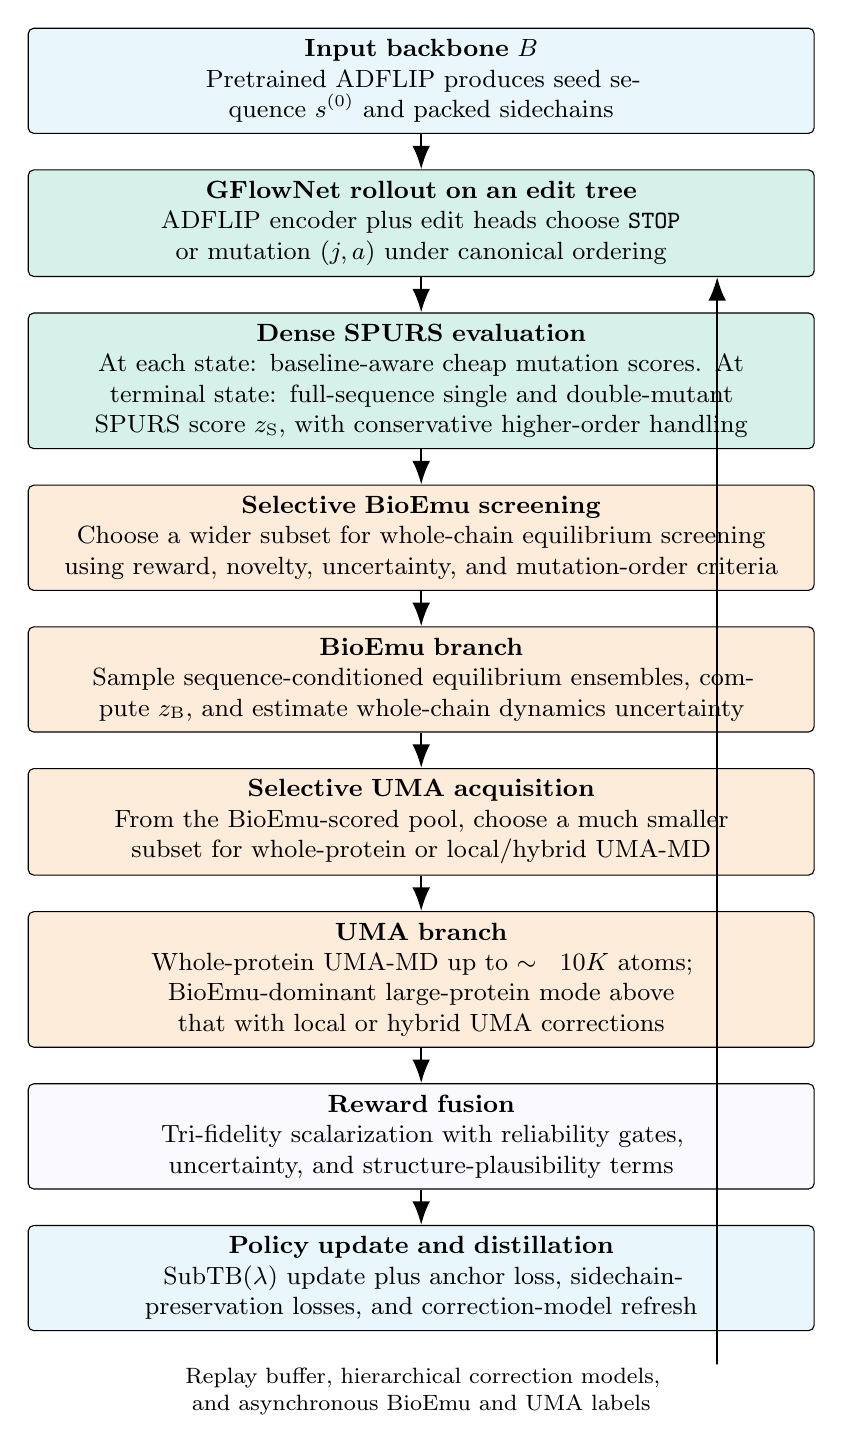
\begin{tikzpicture}[
    node distance=0.45cm,
    every node/.style={font=\small},
    box/.style={draw, rounded corners=2pt, align=center, text width=0.80\linewidth, minimum height=0.8cm, inner sep=4pt},
    bluebox/.style={box, fill=SkyBlue!18},
    greenbox/.style={box, fill=Emerald!16},
    orangebox/.style={box, fill=Apricot!22},
    redbox/.style={box, fill=Lavender!20},
    arr/.style={-{Latex[length=3mm]}, thick}
]
\node[bluebox] (b1) {\textbf{Input backbone $B$}\\Pretrained ADFLIP produces seed sequence $s^{(0)}$ and packed sidechains};
\node[greenbox, below=of b1] (b2) {\textbf{GFlowNet rollout on an edit tree}\\ADFLIP encoder plus edit heads choose \texttt{STOP} or mutation $(j,a)$ under canonical ordering};
\node[greenbox, below=of b2] (b3) {\textbf{Dense SPURS evaluation}\\At each state: baseline-aware cheap mutation scores. At terminal state: full-sequence single and double-mutant SPURS score $z_{\mathrm S}$, with conservative higher-order handling};
\node[orangebox, below=of b3] (b4) {\textbf{Selective BioEmu screening}\\Choose a wider subset for whole-chain equilibrium screening using reward, novelty, uncertainty, and mutation-order criteria};
\node[orangebox, below=of b4] (b5) {\textbf{BioEmu branch}\\Sample sequence-conditioned equilibrium ensembles, compute $z_{\mathrm B}$, and estimate whole-chain dynamics uncertainty};
\node[orangebox, below=of b5] (b6) {\textbf{Selective UMA acquisition}\\From the BioEmu-scored pool, choose a much smaller subset for whole-protein or local/hybrid UMA-MD};
\node[orangebox, below=of b6] (b7) {\textbf{UMA branch}\\Whole-protein UMA-MD up to $\sim 10K$ atoms; BioEmu-dominant large-protein mode above that with local or hybrid UMA corrections};
\node[redbox, below=of b7] (b8) {\textbf{Reward fusion}\\Tri-fidelity scalarization with reliability gates, uncertainty, and structure-plausibility terms};
\node[bluebox, below=of b8] (b9) {\textbf{Policy update and distillation}\\$\SubTB(\lambda)$ update plus anchor loss, sidechain-preservation losses, and correction-model refresh};
\draw[arr] (b1) -- (b2);
\draw[arr] (b2) -- (b3);
\draw[arr] (b3) -- (b4);
\draw[arr] (b4) -- (b5);
\draw[arr] (b5) -- (b6);
\draw[arr] (b6) -- (b7);
\draw[arr] (b7) -- (b8);
\draw[arr] (b8) -- (b9);
\draw[arr] ([xshift=0.31\linewidth]b9.south) |- ++(0,-0.42) -| ([xshift=0.31\linewidth]b2.south);
\node[align=center, text width=0.62\linewidth, font=\footnotesize, below=0.35cm of b9] {Replay buffer, hierarchical correction models, and asynchronous BioEmu and UMA labels};
\end{tikzpicture}
\caption{Vertical overview of \methodI{}, the simultaneous tri-fidelity training loop. SPURS is dense and cheap, BioEmu is wider and dynamics-aware, and UMA is sparse but physically richer.}
\label{fig:simultaneous}
\end{figure}


\subsection{Two-stage acquisition for BioEmu and UMA}

Not every sampled candidate should be sent to every oracle. We therefore define a wider BioEmu acquisition score
\begin{equation}
\label{eq:acqbioemu}
    A_{\mathrm B}(x)=\alpha_1 z_{\mathrm S}^{\mathrm{risk}}(x)+\alpha_2 \sigma_{\mathrm S}(x)+\alpha_3 d_{\mathrm{nov}}(x)+\alpha_4 u_{\mathrm{pack}}(x)+\alpha_5 \mathbf{1}[K(x)=2]+\alpha_6 \frac{K(x)}{L},
\end{equation}
where $\sigma_{\mathrm S}(x)$ is SPURS uncertainty, $d_{\mathrm{nov}}(x)$ is novelty relative to the already screened pool, and $u_{\mathrm{pack}}(x)$ is an optional pack-uncertainty term derived from \packunc. A simple default is $(\alpha_1,\alpha_2,\alpha_3,\alpha_4,\alpha_5,\alpha_6)=(0.40,0.15,0.15,0.10,0.10,0.10)$. This rule deliberately allocates part of the BioEmu budget to uncertain, novel, explicit double-mutant, and higher-order candidates, not only to the top SPURS scorers.

From the BioEmu-scored pool, define a tighter UMA acquisition score
\begin{equation}
\label{eq:acquma}
\begin{aligned}
    A_{\mathrm U}(x)={}&\beta_1 z_{\mathrm B}^{\mathrm{risk}}(x)+\beta_2 \sigma_{\mathrm B}(x)+\beta_3 \big|z_{\mathrm B}^{\mathrm{risk}}(x)-z_{\mathrm S}^{\mathrm{risk}}(x)\big|+\beta_4 d_{\mathrm{nov}}(x)\\
    &+\beta_5 \mathbf{1}[N_{\mathrm{atom}}(x)\leq 10000]+\beta_6 \mathbf{1}[K(x)\ge 3],
\end{aligned}
\end{equation}
with a sensible starting point $(\beta_1,\ldots,\beta_6)=(0.35,0.15,0.20,0.10,0.10,0.10)$. The disagreement term is important: candidates that look good to SPURS but unstable to BioEmu, or vice versa, are often precisely the ones that most benefit from MLIP-based rescoring. If $N_{\mathrm{atom}}(x)$ exceeds the preferred whole-protein UMA paradigm, the final indicator is replaced by a smaller value and the candidate is only sent to local or hybrid UMA if its BioEmu score and disagreement profile justify the cost.

We recommend a BioEmu evaluation rate between $15\%$ and $50\%$ of sampled terminal candidates depending on available compute, and a UMA evaluation rate between $1\%$ and $5\%$ overall or between $5\%$ and $20\%$ of the BioEmu-scored pool. In early training, a higher BioEmu rate is usually worthwhile because it quickly stabilizes the dynamics signal. UMA can remain sparse from the start.



\subsection{Hierarchical correction models}

Because only a subset of candidates receives direct BioEmu or UMA evaluation, we train hierarchical correction models. The first predicts the BioEmu contribution from dense features,
\begin{equation}
    \widehat z_{\mathrm B}^{\mathrm{corr}}(x)=c_{\phi_{\mathrm B}}\big(z_{\mathrm S}(x),\sigma_{\mathrm S}(x),\overline{\packunc}(x),K(x),\mathbf{1}[K(x)=2],\text{sequence features},\text{cheap structure features}\big).
\end{equation}
The second predicts the UMA contribution from both lower-fidelity branches,
\begin{equation}
\begin{aligned}
    \widehat z_{\mathrm U}^{\mathrm{corr}}(x)=c_{\phi_{\mathrm U}}\big(&z_{\mathrm S}(x),z_{\mathrm B}(x),\sigma_{\mathrm S}(x),\sigma_{\mathrm B}(x),\overline{\packunc}(x),\\
    &K(x),\mathbf{1}[K(x)=2],N_{\mathrm{atom}}(x),\rho_{\mathrm B}(x),\rho_{\mathrm U}(x),\text{whole-protein and global structure features}\big).
\end{aligned}
\end{equation}
We recommend starting with ridge ensembles because they remain robust under small label counts and make uncertainty estimation straightforward. If larger labeled sets accumulate, gradient-boosted regressors or shallow neural residual models can replace them.

The key point is hierarchical amortization. BioEmu learns a dynamics correction over SPURS. UMA then learns a physically richer correction over the combination of SPURS and BioEmu. This is substantially better matched to the intended oracle hierarchy than forcing the UMA residual to be predicted directly from SPURS alone.


\subsection{Why \methodI{} can work}

The simultaneous method exploits the asymmetry between the oracles. SPURS annotates and screens a large number of states while ADFLIP itself remains the sole proposal policy. BioEmu supplies whole-chain equilibrium information at a cost low enough to screen a nontrivial fraction of candidates. UMA anchors the reward on a much smaller but strategically chosen subset. The correction models then amortize what the higher-fidelity branches have learned so far. In effect, \methodI{} turns sparse expensive evaluations into a denser supervisory signal while remaining explicit about uncertainty and branch-specific scope.

This method benefits especially from temperature-conditioning. We recommend sampling a reward temperature $\beta\sim\mathrm{Uniform}[0.75,1.75]$ during training. Lower values explore flatter reward distributions and are particularly useful early in training or when the BioEmu and UMA branches are still immature. Higher values increase exploitation once reward fusion is better calibrated. Temperature-conditioning across $\beta$ can be implemented using the logit-scaling strategy of \citet{kim2023lsl-gfn}, although a simpler learned embedding of $\beta$ is also acceptable for a first implementation.


\subsection{Detailed training schedule}

A practical schedule for \methodI{} is as follows.
\begin{enumerate}[leftmargin=1.5em]
    \item \textbf{Baseline and full-redesign warm start.} For each sampled training object, first cache baseline oracle values for the starting undesigned sequence or complex. Then train the ADFLIP policy and newly initialized edit heads with \emph{full fine-tuning} of the non-frozen ADFLIP blocks, using the first full-redesign proposal and single-mutant trajectories under SPURS-only reward. No LoRA is used in the primary schedule.
    \item \textbf{Explicit double-mutant stage.} Up-weight replay from $K=2$ trajectories and introduce SPURS double-mutant epistasis labels on the full candidate sequence. This is the primary cheap-epistasis stage and should be treated as mandatory in the main method.
    \item \textbf{Joint SPURS plus BioEmu phase.} Turn on the BioEmu acquisition branch and the BioEmu correction model. Continue full fine-tuning with \SubTB$(\lambda)$ and the auxiliary losses in Eq.~\eqref{eq:totalloss}. Candidates with $K\ge 3$ are now common, but they are mainly shaped by BioEmu and not by trusted higher-order SPURS supervision.
    \item \textbf{Full tri-fidelity phase.} Turn on UMA acquisition from the BioEmu-screened pool, refresh the UMA correction model periodically, and continue training with the full fused reward. Systems in the $8000$--$10000$ atom range keep UMA active with a soft downweight when calibration weakens; the training corpus does not include systems beyond roughly $10\,000$ atoms.
    \item \textbf{Optional higher-order SPURS ablation.} As an ablation, replace the coarse $K\ge 3$ SPURS statistic with SPURS's own higher-order decoder on the full candidate sequence and repeat the same schedule. This is not part of the primary method.
    \item \textbf{Stabilization phase.} If packing quality degrades, increase the anchor and packing penalties temporarily. If the policy collapses to trivial near-seed sequences, reduce any active radius bias, lower the stop-action prior, or widen the temperature range.
\end{enumerate}
Recommended optimizer defaults are AdamW with learning rate $1\times 10^{-4}$ for newly initialized heads and $2\times 10^{-5}$ to $5\times 10^{-5}$ for the unfrozen pretrained ADFLIP blocks, with cosine decay and $5\%$ warmup. A parameter-efficient LoRA or adapter version should be reported only as an ablation against this full-fine-tuning baseline.

\subsection{Catalytic-oracle augmentation of \methodI{}}

When the task is reaction conditioned, \methodI{} gains a catalytic branch in parallel with the thermostability and binding branches. Let $\mathcal{R}$ be the reaction context for a candidate sequence $x$. The first catalytic acquisition stage mirrors the wide-stage logic already used for BioEmu: annotate a broad set of terminal candidates with a cheap or medium-cost catalytic score before sending only a narrower subset to the structure-aware branch. A simple wide-stage acquisition score is
\begin{equation}
    A_{\mathrm{cat,wide}}(x,\mathcal{R})=
    \alpha^{\mathrm{cat}}_1 d_{\mathrm{nov}}(x)+
    \alpha^{\mathrm{cat}}_2 \packunc(x)+
    \alpha^{\mathrm{cat}}_3 \frac{K(x)}{L}+
    \alpha^{\mathrm{cat}}_4 \mathbf{1}[K(x)\ge 2],
\end{equation}
which favors novel, structurally plausible, and nontrivial edits rather than only trivial near-seed variants. Candidates with valid substrate metadata are eligible for KcatNet, and candidates with valid product or curated missing-modality patterns are also eligible for MMKcat. The resulting KcatNet/MMKcat labels define the wide catalytic screen.

The second catalytic stage is GraphKcat refinement. Define
\begin{equation}
    A_{\mathrm{cat,struct}}(x,\mathcal{R})=
    \beta^{\mathrm{cat}}_1 z_{\mathrm{cat,wide}}^{\mathrm{risk}}(x,\mathcal{R})+
    \beta^{\mathrm{cat}}_2 d_{\mathrm{nov}}(x)+
    \beta^{\mathrm{cat}}_3 \mathbf{1}[K(x)\ge 2],
\end{equation}
where $z_{\mathrm{cat,wide}}^{\mathrm{risk}}$ denotes the fused wide-stage KcatNet/MMKcat score before GraphKcat refinement. Only candidates with admissible protein structure and ligand geometry are sent onward. GraphKcat then provides the pocket-aware $\logkcat$, $\logKm$, and $\logeff$ channels, which are fused through Eq.~\eqref{eq:catfusion}. In other words, catalytic training in \methodI{} mirrors the stability stack structurally: a dense wide screen first, then a narrower structure-aware refinement stage, then unified reward fusion.

\section{Method II: sequential curriculum from cheap exploration to dynamics and catalytic refinement}
\label{sec:method2}

\subsection{Conceptual overview}

\methodII{} is the staged alternative to \methodI{}. Instead of exposing every oracle family throughout a single online optimization loop, it introduces them in sequence. The cheap stage first establishes broad coverage with SPURS and, on catalytic tasks, KcatNet or MMKcat. The middle stage then introduces BioEmu or wide catalytic fusion, depending on whether the task is stability dominated or reaction conditioned. The final stage introduces the narrowest structure-aware branches: UMA for physical stability refinement and GraphKcat for pocket-aware kinetic refinement. This staged view is especially attractive when the narrow branches are scarce, slow, or not yet trustworthy enough to shape the full replay from the beginning.

\subsection{Pseudocode}

\begin{algorithm}[H]
\caption{\methodII{}: sequential curriculum from SPURS exploration to BioEmu and UMA refinement}
\label{alg:method2}
\begin{algorithmic}[1]
\Require Pretrained ADFLIP $\theta_0$, SPURS oracle $\mathcal{O}_{\mathrm S}$, BioEmu oracle $\mathcal{O}_{\mathrm B}$, UMA-MD oracle $\mathcal{O}_{\mathrm U}$
\Statex \textbf{Stage 1A: baseline-aware full redesign and single-mutation exploration}
\State Cache oracle values on each starting undesigned example and train the full-finetuned ADFLIP edit GFlowNet with SPURS-based reward only
\Statex \textbf{Stage 1B: explicit double-mutant epistatic stage}
\State Up-weight replay from $K=2$ candidates and train with SPURS full-sequence double-mutant supervision
\State Save model $\theta^{(1)}$ and replay buffer $\mathcal{B}^{(1)}$
\Statex \textbf{Stage 2: BioEmu refinement}
\State Select top and diverse candidates from $\mathcal{B}^{(1)}$, stratified by mutation order and target-conditioning bucket, for BioEmu screening
\State Run BioEmu on the selected pool and calibrate the resulting ensemble-derived score on a held-out calibration set
\State Continue GFlowNet training from $\theta^{(1)}$ using BioEmu-weighted reward and a slightly narrower $\beta$ range
\State Save refined model $\theta^{(2)}$ and replay buffer $\mathcal{B}^{(2)}$
\Statex \textbf{Stage 3: UMA refinement}
\State Select top and disagreement-rich candidates from $\mathcal{B}^{(2)}$ for direct UMA evaluation
\State Run whole-protein UMA-MD for candidates in the working size setting and local or hybrid fallback otherwise; calibrate the resulting thermostability score on a held-out calibration set
\State Continue GFlowNet training from $\theta^{(2)}$ using BioEmu-plus-UMA weighted reward and the narrowest $\beta$ range
\Statex \textbf{Stage 4: optional deployment distillation}
\State Distill reward-weighted high-scoring candidates into ADFLIP's native sequence head if a fast deployable generator is desired
\end{algorithmic}
\end{algorithm}


\section{Method III: round-based active learning with a one-shot ADFLIP student}
\label{sec:method3}

\subsection{Why a third method is needed}

The first two methods in this manuscript are edit-trajectory methods. They are appropriate when the user wants an explicit mutation path, when per-step credit assignment is central, or when the dynamics oracles can be integrated naturally into or after an edit policy. There is, however, a second use case that deserves a different design: high-throughput proposal generation across many backbones, where the final deployment system should output complete multi-mutant variants in a single forward pass rather than by walking an edit tree.

That use case is directly connected to earlier biological sequence-design work with GFlowNets. Jain et al.~proposed a round-based active-learning algorithm in which a GFlowNet acts as a generator of diverse biological sequences, is trained from both reward evaluations and off-policy trajectories reconstructed from an existing dataset, and is coupled to uncertainty-aware acquisition so that each round proposes a diverse, informative batch rather than a single maximizer \citep{jain2022bioseqgfn}. In the same paper, the authors explicitly identified non-autoregressive generators and multi-oracle outer loops as natural future extensions \citep{jain2022bioseqgfn}. The original GFlowNet paper also framed the approach as non-iterative diverse candidate generation in the sense that search is amortized during training and i.i.d. samples can then be drawn rapidly at deployment \citep{bengio2021noniter}. \methodIII{} is the adaptation of that idea to ADFLIP, SPURS, BioEmu, UMA, and the catalytic-oracle bundle.

The key distinction is the following. The \emph{ideal} \methodIII{} uses a GFlowNet internally as the reward-proportional teacher, because the target distribution over complete sequences is multimodal and expensive. But the deployed proposal model is a one-shot student. For a given backbone and seed sequence, it predicts mutation count, mutation locations, and replacement residues in parallel, then runs a single structural realization step. There is no edit-time tree walk at deployment. This makes the method attractive when one wants to screen many candidate proteins or when a downstream workflow prefers a single precomputed batch per design round.

The current repository implementation now instantiates the teacher as a real trajectory-balance GFlowNet over the canonical edit DAG. Let $\tau=(s_0\rightarrow s_1\rightarrow\cdots\rightarrow s_T=x)$ denote the canonical edit trajectory from the baseline seed to terminal candidate $x$, where each nonterminal action factorizes into \texttt{STOP} / \texttt{continue}, a position choice, and a replacement-residue choice. The implemented forward policy is
\begin{equation}
    \PF_\theta(a_t\mid s_t)=
    \PF_\theta(\mathtt{STOP}\mid s_t)
    \quad\text{or}\quad
    \PF_\theta(\neg\mathtt{STOP}\mid s_t)\,
    \PF_\theta(j_t\mid s_t,\neg\mathtt{STOP})\,
    \PF_\theta(a_t^{\mathrm{aa}}\mid j_t,s_t,\neg\mathtt{STOP}),
\end{equation}
with deterministic backward reconstruction under canonical edit ordering. The teacher is trained with a trajectory-balance residual
\begin{equation}
    \mathcal{L}_{\mathrm{TB}}(\tau)
    =
    \Bigg(
        \log Z_\theta(s_0)
        + \sum_{t=0}^{T-1}\log \PF_\theta(a_t\mid s_t)
        - \log R_r(x)
    \Bigg)^2,
\end{equation}
where $R_r(x)>0$ is the round-$r$ scalar reward or risk-adjusted surrogate reward. Off-policy trajectories are reconstructed from labeled candidates in $D_r$, and on-policy trajectories are sampled from the teacher itself and scored with the current surrogate ensemble. The one-shot student is then distilled from actual teacher samples rather than from empirical frequency tables. This means the repository path now matches the mathematical intent of \methodIII{}: reward-proportional training happens on an explicit trajectory model, while deployment remains one shot.

\subsection{Conceptual structure}

\methodIII{} has four trainable or updatable components per active-learning round $r$:
\begin{enumerate}[leftmargin=1.5em]
    \item a \textbf{surrogate ensemble} $M_r$ that predicts the fused thermostability target and its epistemic uncertainty from backbone, seed sequence, and candidate sequence;
    \item a \textbf{trajectory-balance teacher policy} $\pi_{\theta,r}$ over canonical edit trajectories;
    \item a \textbf{one-shot ADFLIP student} $q_{\phi,r}$ that learns to imitate the teacher's terminal distribution without explicit edit-time iteration;
    \item a \textbf{triage stack} in which SPURS is run densely, BioEmu on a wider filtered subset, and UMA on a smaller high-value subset.
\end{enumerate}
The surrogate is needed because an active-learning round should be able to score many candidate sequences cheaply. The teacher is needed because reward-proportional exploration over multi-mutant sequence space is the core reason to use a GFlowNet at all. In the implemented repository path, that role is played by an explicit flow-consistency teacher trained on reconstructed and sampled trajectories rather than by a reward-weighted empirical shortcut. The student is needed because the deployment requirement here is one-shot generation rather than trajectory sampling. In the catalytic specialization, the triage stack becomes packed-structure GraphKcat at the wide prefilter stage and whole-enzyme UMA dynamics on the narrower expensive subset, with fused catalytic labels replacing or augmenting the stability-only reward.

\subsection{Teacher training with off-policy data}

At round $r$, let $D_r$ denote the set of all candidates evaluated so far with whichever oracle bundle was available. Teacher training uses both on-policy rollouts and off-policy reconstructed trajectories from the evaluated dataset \citep{jain2022bioseqgfn}. For each sequence in $D_r$, reconstruct a canonical edit trajectory relative to its seed sequence. If a candidate is $K$ mutations away from the seed, the reconstructed trajectory contains exactly those $K$ edits in canonical order followed by stop. These off-policy trajectories stabilize training, improve local support around already interesting mutants, and make efficient use of expensive labels.

The implemented repository path now follows this construction directly. The teacher maintains a learnable $\log Z$ for each seed family, a stop policy over edit depth, seed-conditioned position logits, and residue-replacement logits conditioned on the original residue identity. This is a deliberately compact parameterization, but it is still a genuine GFlowNet teacher because the optimization target is the trajectory-balance residual on explicit trajectories. On-policy teacher rollouts are scored with the current surrogate ensemble, yielding positive surrogate rewards that play the same role as expensive labels but at lower cost.

We recommend a mixture ratio $\gamma_{\mathrm{off}}\in[0.25,0.60]$ between offline reconstructed trajectories and on-policy teacher rollouts, with a default of $0.5$ in early rounds and a decay toward $0.25$ once the student begins proposing genuinely novel high-quality candidates. The current repository path uses trajectory balance rather than \SubTB{}, which is reasonable because the canonical edit teacher is intentionally compact and the average mutation orders in the default catalytic loop remain moderate.

\subsection{One-shot student parameterization}

The one-shot student is designed to generate a full multi-mutant candidate without edit-time iteration. It reuses ADFLIP's multi-scale residue-and-atom encoder but changes the output parameterization. Given a backbone $B$, seed sequence $s^{(0)}$, seed sidechains $X^{\mathrm{sc},(0)}$, and control vector $c$, the student outputs three objects in a single forward pass:
\begin{align}
    p_{\phi}(K\mid B,s^{(0)},c),\qquad
    \ell^{\mathrm{mask}}_{1:L}\in\RR^L,\qquad
    \ell^{\mathrm{aa}}_{1:L}\in\RR^{L\times 20}.
\end{align}
Here $p_{\phi}(K\mid\cdot)$ is a categorical distribution over mutation count, $\ell^{\mathrm{mask}}$ are per-position logits indicating how likely each position is to be mutated, and $\ell^{\mathrm{aa}}$ are replacement-residue logits. The control vector $c$ can include reward temperature, desired quantile of the teacher distribution, protein-level metadata, and an oracle-mixture tag indicating whether the current round is SPURS-heavy, BioEmu-heavy, or UMA-heavy.

Candidate generation proceeds as follows.
\begin{enumerate}[leftmargin=1.5em]
    \item Sample a mutation count $K\sim p_{\phi}(K\mid B,s^{(0)},c)$.
    \item Sample $K$ mutation sites without replacement using Gumbel-top-$K$ on $\ell^{\mathrm{mask}}$.
    \item For each chosen site $j$, sample a replacement residue from the categorical distribution induced by $\ell^{\mathrm{aa}}_j$ after masking out the seed amino acid.
    \item Leave all non-chosen sites unchanged, yielding a complete candidate sequence $x$ in one pass.
    \item Run a single structural realization step: either one ADFLIP masked update restricted to the mutated sites or one sidechain-diffusion packing pass conditioned on the completed sequence.
\end{enumerate}
The resulting candidate is therefore a one-shot multi-mutant proposal. The only iterative computation left is oracle evaluation and any optional post hoc rescoring; there is no edit-time tree walk.

\subsection{Student losses and distillation objective}

Let $\widetilde p_r(x)$ denote the normalized terminal distribution induced by the teacher over a candidate pool $\mathcal{C}_r$, for example a mixture of on-policy teacher samples, replay-buffer elites, and evaluated sequences in $D_r$. The primary distillation loss is a reward-weighted cross-entropy,
\begin{equation}
\label{eq:method3distill}
    \mathcal{L}_{\mathrm{distill}}(\phi)=-\sum_{x\in\mathcal{C}_r} \widetilde p_r(x)\log q_{\phi}(x\mid B,s^{(0)},c),
\end{equation}
where the one-shot probability factorizes as
\begin{equation}
    q_{\phi}(x\mid B,s^{(0)},c)=p_{\phi}(K_x\mid B,s^{(0)},c)\;q_{\phi}(M_x\mid K_x,B,s^{(0)},c)\;q_{\phi}(x_{M_x}\mid M_x,B,s^{(0)},c).
\end{equation}
A practical implementation does not need exact normalization over the full sequence space; it only needs accurate probabilities on the candidate pool. In that setting Eq.~\eqref{eq:method3distill} can be estimated from minibatches of teacher samples and replay items.

We recommend augmenting the distillation loss with four auxiliary terms:
\begin{align}
    \mathcal{L}_{\mathrm{student}} ={}& \lambda_{\mathrm{distill}}\mathcal{L}_{\mathrm{distill}} + \lambda_K\mathcal{L}_{K} + \lambda_{\mathrm{rank}}\mathcal{L}_{\mathrm{rank}} + \lambda_{\mathrm{anchor}}\mathcal{L}_{\mathrm{anchor}} + \lambda_{\mathrm{side}}\mathcal{L}_{\mathrm{side}}.
\end{align}
\begin{itemize}[leftmargin=1.5em]
    \item $\mathcal{L}_K$ is a count-calibration loss on $p_{\phi}(K\mid\cdot)$ using teacher samples and evaluated sequences.
    \item $\mathcal{L}_{\mathrm{rank}}$ is a pairwise ranking loss so that candidates with higher fused reward receive larger student log-probability than nearby lower-reward candidates from the same backbone.
    \item $\mathcal{L}_{\mathrm{anchor}}$ keeps the student close to the pretrained ADFLIP denoising distribution on unedited or lightly edited seeds to avoid structural drift.
    \item $\mathcal{L}_{\mathrm{side}}$ preserves packing quality on the realized candidate structures through clash and packing-consistency penalties.
\end{itemize}
A good default is $(\lambda_{\mathrm{distill}},\lambda_K,\lambda_{\mathrm{rank}},\lambda_{\mathrm{anchor}},\lambda_{\mathrm{side}})=(1.0,0.2,0.25,0.5,0.2)$, but these weights should be tuned on held-out backbones.

\subsection{Round structure and evaluation budget}

A typical \methodIII{} run uses 5--15 active-learning rounds. Each round has six stages.
\begin{enumerate}[leftmargin=1.5em]
    \item Fit or update the surrogate ensemble $M_r$ on $D_r$.
    \item Train the teacher policy as a trajectory-balance GFlowNet with acquisition reward $R_r$ and a mixture of off-policy reconstructed trajectories and on-policy surrogate-scored rollouts.
    \item Distill the teacher into the one-shot student $q_{\phi,r}$.
    \item Sample a large candidate pool from the student, for example $10^4$--$10^5$ candidates across the current backbone minibatch, then filter by chemistry, structure (matching the starting backbone, and with desirable properties such as being well-packed), sequence diversity, and novelty.
    \item Run SPURS on all filtered candidates and BioEmu on a larger prioritized subset.
    \item Evaluate a compact diverse subset with UMA, append results to $D_{r+1}$, and continue.
\end{enumerate}
The highest-fidelity evaluation budget is therefore controlled at the round level rather than the step level. This matches the biological-sequence active-learning workflow in Jain et al.~more closely than Methods I and II do \citep{jain2022bioseqgfn}. It is often the right choice when the expensive branch has low throughput.

The default selection rule for the BioEmu and UMA batches is cluster-balanced top-$b$. First cluster candidates by sequence identity or mutation-set Jaccard distance. Then within each cluster rank by acquisition score, with an additional preference for higher-order candidates that have not yet received BioEmu or UMA supervision. Use the wider quota for BioEmu and the narrower quota for UMA. This keeps batch diversity high while still favoring high acquisition. In the large-protein setting, it is perfectly reasonable for every selected candidate to receive BioEmu but only a small fraction to receive local or hybrid UMA.

\subsection{Why \methodIII{} is genuinely non-iterative at deployment}

The GFlowNet teacher remains sequential internally; that is unavoidable because reward-proportional training for compositional discrete objects is naturally expressed on a DAG. The implemented repository path keeps that sequential structure inside the teacher and collapses it only at the student-distillation stage, where teacher samples are summarized into one-shot student outputs. The user-facing generation mechanism therefore remains non-iterative in the practically relevant sense. Once a round is complete, the student produces a complete multi-mutant proposal in one forward pass and one structural realization step. Compared with Methods I and II, this changes three things.
\begin{enumerate}[leftmargin=1.5em]
    \item \textbf{Latency:} proposal generation becomes much faster for large screening batches.
    \item \textbf{Engineering simplicity:} deployment no longer needs replay buffers, online reward correction, or tree traversal.
    \item \textbf{Loss of edit-path interpretability:} the student outputs the terminal sequence directly, so explicit trajectory-level explanations are weaker unless one also stores the teacher distribution for attribution.
\end{enumerate}
A practical deployment stack can still run SPURS on the full proposal batch, BioEmu on a filtered subset, and UMA only on the top handful, without changing the fact that the proposal model itself is one-shot.

\subsection{Pseudocode}

\begin{algorithm}[H]
\caption{\methodIII{}: active-learning teacher policy with one-shot ADFLIP student}
\label{alg:method3}
\begin{algorithmic}[1]
\Require Initial dataset $D_0$, pretrained ADFLIP parameters $\theta_0$, student parameters $\phi_0$, round budget $R$, BioEmu batch size $b_{\mathrm B}$, UMA batch size $b_{\mathrm U}$
\For{$r=0$ to $R-1$}
    \State Fit surrogate ensemble $M_r$ on $D_r$ to obtain mean $\mu_r(x)$ and uncertainty $\sigma_r(x)$
    \State Define acquisition-based reward $R_r(x)$ from $\mu_r(x)$, $\sigma_r(x)$, diversity penalties, and validity filters
    \State Train teacher policy for round $r$ as a trajectory-balance GFlowNet using reconstructed off-policy trajectories and surrogate-scored on-policy rollouts
    \State Build candidate pool $\mathcal{C}_r$ from teacher samples, replay elites, and evaluated sequences
    \State Distill teacher distribution on $\mathcal{C}_r$ into one-shot student $q_{\phi,r}$
    \State Sample a large proposal batch $B_r$ from $q_{\phi,r}$ in one pass per backbone
    \State Repack mutated sidechains once, optional BioEmu RMSD validation, and discard invalid structures
    \State Rescore surviving candidates with SPURS and the surrogate
    \State Select a diverse subset of size $b_{\mathrm B}$ and run BioEmu to obtain whole-chain dynamics scores
    \State From the BioEmu-scored pool, select a smaller diverse subset of size $b_{\mathrm U}$ for UMA
    \For{each selected candidate $x$}
        \If{prepared system fits the whole-protein UMA budget}
            \State Run whole-protein UMA-MD ladder and compute calibrated expensive score
        \Else
            \State Run local or hybrid UMA fallback and compute calibrated expensive score
        \EndIf
        \State Add evaluated tuple for $x$ to $D_{r+1}$
    \EndFor
\EndFor
\State Return final one-shot student $q_{\phi,R}$, teacher replay buffer, and evaluated dataset $D_R$
\end{algorithmic}
\end{algorithm}

\subsection{Catalytic active learning with whole-enzyme UMA and GraphKcat}

The catalytic specialization of \methodIII{} uses the same teacher-student structure but changes the oracle stack and the physical interpretation of the expensive stage. Each candidate is paired with a reaction context $\mathcal{R}$ and, in the default implemented repository path, with two endpoint structures: a reactant-bound complex and a product-bound complex. The surrogate ensemble predicts a fused catalytic score rather than only a thermostability score. The teacher then assigns reward-weighted probability mass to catalytic candidates, and the deployed student remains one shot: it proposes a full enzyme variant in one forward pass, after which packed-structure GraphKcat and whole-enzyme UMA dynamics determine whether the candidate is worth retaining.

The local repository already implements a concrete self-contained orchestration of this pattern. The current round runner first validates that each example carries substrate metadata, endpoint complex paths, protein chain identifiers, and pocket positions. It then trains or refreshes the surrogate, trajectory-balance teacher, and one-shot student, generates a candidate pool, repacks the full pool on endpoint complexes with LigandMPNN, runs packed-structure GraphKcat across that pool, keeps the top GraphKcat tranche, selects a catalytic batch from within that screened set, runs the broad whole-enzyme UMA screen, runs forward and reverse steered UMA dynamics, optionally launches a path umbrella PMF, fuses the resulting catalytic labels, and finally appends those labels to the active-learning dataset. The mathematical abstraction is the same as in the generic \methodIII{} loop, but the concrete oracle routing is now explicitly dynamical rather than only predictive.

The corresponding catalytic acquisition scores reflect this asymmetry. For the broad catalytic stage we recommend
\begin{equation}
    A_{\mathrm{UCAT}}(x,\mathcal{R})=
    \alpha^{\mathrm{UCAT}}_1 d_{\mathrm{nov}}(x)+
    \alpha^{\mathrm{UCAT}}_2 \packunc(x)+
    \alpha^{\mathrm{UCAT}}_3 \frac{K(x)}{L}+
    \alpha^{\mathrm{UCAT}}_4 \mathbf{1}[K(x)\ge 2],
\end{equation}
which preserves diversity and mutation-order coverage before the expensive catalytic screen. For the narrower GraphKcat stage we recommend
\begin{equation}
    A_{\mathrm{GK}}(x,\mathcal{R})=
    \beta^{\mathrm{GK}}_1 z_{\mathrm{UCAT}}^{\mathrm{risk}}(x,\mathcal{R})+
    \beta^{\mathrm{GK}}_2 d_{\mathrm{nov}}(x)+
    \beta^{\mathrm{GK}}_3 \mathbf{1}[K(x)\ge 2].
\end{equation}
Only candidates whose protein structure and ligand geometry can be materialized are eligible for GraphKcat. This design keeps the narrower learned catalytic branch focused on cases where its structural inductive bias is actually usable, while the broad dynamical stage remains the default source of catalytic signal.

\begin{algorithm}[H]
\caption{Catalytic \methodIII{} round with whole-enzyme UMA and GraphKcat}
\label{alg:method3_kcat}
\begin{algorithmic}[1]
\Require Active-learning dataset $D_r$, reaction metadata, docked reactant-bound and product-bound endpoint complexes, pretrained generator, broad UMA-cat budget $b_{\mathrm{UCAT}}$, narrower GraphKcat budget $b_{\mathrm{GK}}$
\State Validate substrate metadata, endpoint complex paths, protein chain IDs, and pocket positions
\State Fit surrogate ensemble $M_r$ on fused catalytic labels from prior rounds
    \State Train teacher policy on catalytic or joint catalytic-stability reward as a trajectory-balance GFlowNet over canonical edit trajectories
\State Distill teacher terminal distribution into one-shot student $q_{\phi,r}$
\State Sample a large candidate pool from $q_{\phi,r}$ and apply structural plausibility filters
\State Select a broad candidate subset by $A_{\mathrm{UCAT}}$
\State Repack each selected candidate onto reactant-bound and product-bound complexes with LigandMPNN
\State Run whole-enzyme UMA equilibrium screening on the reactant-bound complexes to estimate productive-pose occupancy and $\widehat{\Delta G}_{\mathrm{gate}}$
\State Run forward and reverse steered whole-enzyme UMA dynamics between the reactant-bound and product-bound complexes
\State Optionally seed a path umbrella PMF from the steered trajectories and estimate $\widehat{\Delta G}_{\mathrm{PMF}}^\ddagger$
\State Convert the catalytic dynamics outputs into $\widehat \ell_{\mathrm{UMAcat}}$ through Eq.~\eqref{eq:ucatproxy}
\State Select a narrower structure-qualified subset by $A_{\mathrm{GK}}$ and run GraphKcat
\State Fuse UMA-cat and GraphKcat through Eq.~\eqref{eq:catfusion} to obtain catalytic rewards
\State Append the newly labeled tuples to $D_{r+1}$ and continue to the next round
\end{algorithmic}
\end{algorithm}

\subsection{Recommended defaults for the first implementation}

For a first implementation of \methodIII{}, we recommend 8 active-learning rounds, a teacher-training phase of 20k--40k gradient steps per round, and a student-distillation phase of 10k--20k steps per round. Use 8--16 surrogate ensemble members if compute allows; otherwise use 4 members and increase the conservative exploration bonus $\kappa_r$. Set the default round budget so that every selected candidate receives SPURS, at least 20--40\% of the filtered round pool receives BioEmu, and at least 30\% of the UMA batch comes from candidates whose mutation order exceeds the median mutation order in $D_r$. This prevents the active-learning loop from collapsing to small edits. Use a higher off-policy fraction in the first two rounds and decay it later. Because the student is one-shot, it is worth oversampling candidate proposals during rounds 4--8 and tightening cluster-based selection rather than narrowing the student itself too early.

\subsection{Instrumentation, logging, and reproducibility}

Multi-oracle active learning is difficult to debug if observability is treated as an afterthought. We therefore recommend that every round expose both optimization diagnostics and oracle-stage diagnostics as first-class outputs. In the current repository implementation, this instrumentation is not merely advisory; it is part of the default runtime path. Let $u$ index teacher updates and let $v$ index student-distillation updates. The teacher logs a telemetry vector
\begin{equation}
    m_u^{\mathrm{teacher}}=
    \big(
        \mathcal{L}_{\mathrm{TB}},
        \mathcal{L}_{\mathrm{off}},
        \mathcal{L}_{\mathrm{on}},
        \mathcal{L}_{\mathrm{reg}},
        \delta_{\mathrm{abs}},
        \|\nabla\|_{\mathrm{pre}},
        \|\nabla\|_{\mathrm{post}},
        \bar p_{\mathrm{stop}},
        \overline{\log Z},
        \eta
    \big)_u,
\end{equation}
where $\eta$ is the learning rate and $\delta_{\mathrm{abs}}$ is the absolute TB residual. The student logs
\begin{equation}
    m_v^{\mathrm{student}}=
    \big(
        f_{\mathrm{sampled}},
        \EE[K],
        H[K],
        N_{\mathrm{distinct}\,K},
        N_{\mathrm{seed\,families}}
    \big)_v,
\end{equation}
which exposes whether the one-shot distillation path is collapsing to a narrow mutation-order regime or a narrow set of seed families. The surrogate logs bootstrap-level statistics rather than only a final checkpoint summary, allowing the user to detect whether the ensemble members are seeing materially different resampled data.

The same principle applies to the oracle stages. For each stage $\mathcal{O}\in\{\mathrm{GraphKcat},\mathrm{UMAcat}\}$, the repository now emits a structured summary
\begin{equation}
    m_r^{\mathcal{O}}=
    \big(
        N_{\mathrm{attempted}},
        N_{\mathrm{ok}},
        f_{\mathrm{ok}},
        \EE[\hat y_{\mathcal{O}}],
        \Var[\hat y_{\mathcal{O}}],
        \text{stage-specific failure counts}
    \big)_r,
\end{equation}
for each active-learning round $r$. At the round level, the orchestration layer also records gate outcomes, append summaries, and teacher-student evaluation summaries. The intended use is twofold. First, these quantities make training failures diagnosable rather than anecdotal. Second, they make experimental reporting more credible because a later empirical paper can distinguish optimization failure, oracle failure, and data-censoring failure rather than collapsing them into a single negative result.

In the repository implementation, these telemetry streams are written both to structured JSON/JSONL artifacts and to Weights \& Biases. The default runtime uses an automatic W\&B mode: it syncs online when credentials are available and falls back to offline artifact logging otherwise, so that telemetry is preserved on both connected and restricted machines. Progress reporting is likewise layered: an experiment-level progress bar tracks rounds, a round-level progress bar tracks orchestration stages, and the trainer and oracle subprocesses expose their own detailed progress bars or heartbeat-style logs. This is a mundane implementation detail compared with the oracle physics, but it is essential if the methodology is to be reproducible and if expensive catalytic runs are to be trusted rather than guessed at.

\subsection{Expected strengths and likely failure modes}

\methodIII{} should excel when the lab needs large, diverse proposal batches and the highest-fidelity oracle can only be queried in coarse rounds. It is also well aligned with industrial screening workflows, where one often wants tens of thousands of proposals reduced to a few hundred computationally filtered sequences and then a few dozen experimental candidates. The main risk is student undercoverage of thin but valuable teacher modes, especially at high mutation order. That risk is manageable if the round-level evaluation keeps measuring teacher-student KL on held-out candidate pools and if the student is retrained whenever that gap widens beyond a preset tolerance.

A second risk is that the one-shot factorization of mutation count, mask, and amino-acid identities may underrepresent long-range dependencies that an edit-trajectory policy captures naturally. When this happens, one can either enrich the student with low-rank pairwise coupling heads over mutated sites or allow a tiny fixed number of masked refinement passes after the initial one-shot proposal. The latter does not change the core character of the method: the student remains a one-shot proposer, and any refinement is a bounded post-processing step rather than a sequential search policy.


\section{BioEmu protocol as a fast dynamics oracle and large-protein complement}
\label{sec:bioemu}

\subsection{Why a dedicated BioEmu protocol is required}

BioEmu is not merely another scalar stability regressor. It is a sequence-conditioned generative equilibrium-ensemble model \citep{lewis2024bioemu}. That changes how it should be integrated into a design pipeline. A scalar predictor can be dropped into a reward function with only calibration and uncertainty estimation. An equilibrium-ensemble model provides a much richer object: a distribution over backbone conformations. The challenge is to transform that ensemble into a scientifically meaningful thermostability signal that is aligned with the fixed target backbone and with the multi-mutant design objective of the present manuscript.

The BioEmu paper provides strong motivation for this effort. It reports that BioEmu can generate thousands of statistically independent samples from a protein structure ensemble per hour on a single GPU, that it qualitatively captures conformational changes such as domain motions, local unfolding, and cryptic-pocket formation, and that it quantitatively matches equilibrium observables with free-energy errors on the order of $1$ kcal/mol in several benchmark settings \citep{lewis2024bioemu}. The same paper also reports direct stability prediction through generated ensembles, with folding free-energy mean absolute error below $0.8$ kcal/mol on its train/test splits \citep{lewis2024bioemu}. These are precisely the properties that make BioEmu attractive as a fast dynamics oracle.

\subsection{Eligibility and scope}

The protocol in this manuscript uses BioEmu only where the model's public evidence supports it. The default BioEmu-eligible setting is:
\begin{enumerate}[leftmargin=1.5em]
    \item soluble proteins or chain-wise approximations of larger systems;
    \item single-chain proteins, or multi-chain settings reduced to a designated design chain when the missing partners are not expected to dominate the fold;
    \item no essential membrane environment and no stability mechanism that fundamentally depends on an explicit ligand absent from the BioEmu input.
\end{enumerate}
If any of these conditions fail, BioEmu should be treated as a weak exploratory prior or omitted entirely. This is not a weakness of the methodology; it is explicit scope control.

Within that scope, BioEmu is especially useful for proteins whose prepared all-atom systems exceed roughly $8000$--$10000$ atoms. In that setting, one often still wants a whole-chain dynamics signal, but forcing every candidate through whole-protein UMA-MD may be scientifically or computationally inefficient. BioEmu is then the natural first-line dynamics oracle, with UMA reserved for local or hybrid follow-up for larger system until it is validated further.

\subsection{From BioEmu samples to thermostability features}

Given candidate sequence $s$, generate $M_{\mathrm B}$ BioEmu samples
\[
\mathcal{Y}(x)=\{y_m\}_{m=1}^{M_{\mathrm B}}, \qquad y_m \sim p_{\mathrm{BioEmu}}(\cdot\mid s).
\]
For training-time ranking, we recommend $M_{\mathrm B}=2048$ by default. For shortlisted candidates or calibration experiments, $M_{\mathrm B}=10{,}000$ is a sensible target because the BioEmu paper itself uses $10$k-sample ensembles in several analyses \citep{lewis2024bioemu}. Each sample is compared to the target backbone using the observables defined earlier:
\[
Q_{\mathrm{nat}}^{\mathrm B},\quad \mathrm{RMSD}_{\mathrm{bb}}^{\mathrm B},\quad H_{\mathrm{sec}}^{\mathrm B},\quad R_g^{\mathrm B},\quad U_b^{\mathrm B}.
\]
The first four define global fold retention. The block-local unfolding scores $U_b^{\mathrm B}$ define where the ensemble destabilizes relative to the mutation pattern. We also recommend recording optional motif-specific indicators such as loop opening, hinge variance, or pocket-volume proxies whenever the target fold class makes them relevant.

The core BioEmu stability statistic is the two-basin estimator in Eq.~\eqref{eq:bioemu_twostate}. However, the full feature vector
\[
u_{\mathrm B}(x)=\Big[\widehat{\dG}^{\mathrm{BioEmu}}_{\mathrm{stab}},\ p_{\mathcal F}^{\mathrm B},\ p_{\mathcal U}^{\mathrm B},\ \overline{Q_{\mathrm{nat}}^{\mathrm B}},\ \overline{H_{\mathrm{sec}}^{\mathrm B}},\ \overline{R_g^{\mathrm B}},\ \max_b \overline{U_b^{\mathrm B}},\ \mathrm{Var}(R_g^{\mathrm B})\Big]
\]
is more informative for calibration. In particular, it is common to see candidates with similar folded-basin occupancy but very different local-unfolding behavior around mutated regions. Those candidates should not be treated as thermodynamically equivalent for design purposes.

\subsection{Calibration and uncertainty}

Calibrate BioEmu-derived features to experimental stability on held-out proteins. We recommend a monotone regressor as the default because one expects, all else equal, larger folded-basin occupancy and higher contact retention to imply greater stability. If training data are sparse, ridge regression with spline features is a strong baseline. If larger calibration sets are available, monotone gradient-boosted trees are attractive.

Uncertainty should combine at least three components:
\begin{enumerate}[leftmargin=1.5em]
    \item \textbf{Sample uncertainty:} bootstrap variance over the finite BioEmu sample set.
    \item \textbf{Model uncertainty:} checkpoint or ensemble disagreement if multiple BioEmu parameter snapshots are retained.
    \item \textbf{Classifier uncertainty:} threshold sensitivity of the folded/disrupted basin definition.
\end{enumerate}
Candidates with high BioEmu uncertainty should not be discarded automatically. They are often precisely the ones worth sending to UMA, because disagreement between a fast equilibrium emulator and a local or global MLIP-MD refinement is informative.

\subsection{How BioEmu and UMA interact above the whole-protein UMA setting}

For proteins whose prepared systems exceed roughly $8000$--$10000$ atoms, the recommended dynamic-screen workflow is:
\begin{enumerate}[leftmargin=1.5em]
    \item run SPURS densely to define the local mutation landscape;
    \item run BioEmu on the widest feasible filtered candidate pool to obtain whole-chain equilibrium diagnostics;
    \item select a small subset for local or hybrid UMA based on BioEmu score, BioEmu-SPURS disagreement, mutation order, and mechanistic interest;
    \item fuse the three branches with reliability gating so that BioEmu carries the dominant whole-chain dynamics weight and UMA contributes targeted physical corrections.
\end{enumerate}

\section{UMA-MD protocol as the high-fidelity oracle}
\label{sec:uma}

\subsection{Why a dedicated UMA protocol is still required}

It is tempting to say ``run UMA MD on the protein and read off $\dG$.'' That is not rigorous enough. Thermostability is a free-energy property. Even with a strong MLIP, $\dG$ depends on sampling, basin definitions, protonation handling, environment specification, and the system-size setting in which the model is deployed. The purpose of this section is to spell out a protocol that is technically defensible and aligned with the requirement that UMA be used on whole proteins whenever practical, while also explaining exactly where BioEmu should take over as the main whole-chain dynamics oracle.

The strongest published facts we can lean on are the following. OMol25 consists of more than $100$ million DFT calculations at the $\omega$B97M-V/def2-TZVPD level, with broad chemistry including biomolecules and explicit solvation, and systems up to $\sim 350$ atoms \citep{levine2025omol25}. UMA is trained on half a billion unique 3D atomic structures across multiple domains, and a single model can be used through the FAIR Chemistry stack to run domain-specific prediction and MD workflows such as molecular MD under the \texttt{omol} task \citep{wood2025uma,fairchem2025github}. The FAIR Chemistry repository also documents a worked large atom count MD example on $8\times$H100 GPUs and reports current wall-clock MD throughput around $1$ ns/day for $100$k$+$-atom systems \citep{fairchem2025github} on a single H100. This establishes that large-system UMA-MD is computationally feasible.

What remains nontrivial is thermodynamic validity on proteins. The public training data are not a direct benchmark suite for whole-protein folding free energies. We therefore adopt the following principle: use whole-protein UMA-MD up to $\sim 8000-10000$ atoms as the default high-fidelity branch whenever the prepared system fits, but treat the resulting thermodynamic quantities as calibrated stability estimates whose relationship to experimental thermostability must be validated explicitly. Above that scenario, BioEmu is the default whole-chain dynamics oracle and UMA is focused on local or hybrid corrections, unless the context involves multimers or complexes with non-protein systems.

\subsection{Prepared-system definition and default operating scenarios}

We distinguish four operating settings.

\paragraph{Setting A: BioEmu plus whole-protein UMA up to around $8000$ atoms (default).}
If the prepared protein system satisfies $N_{\mathrm{atom}}\leq 8000$ and the protein is BioEmu-eligible, run both whole-chain BioEmu screening and whole-protein UMA-MD. BioEmu helps prioritize which candidates deserve the MLIP-MD budget and provides an independent equilibrium signal. UMA then supplies the higher-fidelity branch.

\paragraph{Setting B: BioEmu-dominant large-protein mode above about $8000$ atoms.}
If the prepared whole-protein system exceeds the atom budget or falls into the $8000$--$10000$-atom gray zone where calibration may weaken, use BioEmu as the primary whole-chain dynamics oracle. UMA is still useful, but should be down-weighted compared to BioEmu unless the system is a complex. 

\paragraph{Setting C: local or hybrid UMA for targeted mechanistic questions.}
Even below the atom budget, some candidates may deserve local mechanistic scrutiny around a mutation cluster, catalytic ion, or particularly uncertain region. Extract a local subsystem, cap bonds, retain first-shell waters or ions if chemically required, and use UMA-MD to estimate local free-energy or structural robustness proxies.

\paragraph{Setting D: BioEmu-ineligible cases.}
If the system fundamentally depends on a membrane, explicit ligand, or multimeric context that BioEmu does not model well, use SPURS plus the appropriate local or hybrid UMA protocol and do not pretend that a BioEmu score exists.

\subsection{Pre-processing, protonation, and system construction}

Every candidate sequence must be converted into a chemically sensible starting structure before UMA-MD begins. We recommend the following sequence of steps.
\begin{enumerate}[leftmargin=1.5em]
    \item Start from the ADFLIP terminal full-atom structure and perform one full cleanup or repacking pass if the mean local \packunc is above threshold.
    \item Assign protonation states at a stated pH (default pH $7.0$) using a deterministic pipeline. Histidine tautomer choices must be cached because they affect charge and local energetics.
    \item Add missing hydrogens and retain cofactors, catalytic waters, or structural ions when these are part of the intended fold or stabilization mechanism.
    \item Compute the prepared-system atom count $N_{\mathrm{atom}}$. If $N_{\mathrm{atom}}\leq 8000$, proceed to setting A whole-protein UMA-MD. If $N_{\mathrm{atom}}>8000$, trigger the BioEmu-dominant large-protein mode, run down-weighted UMA, or only run local or hybrid UMA as needed for more than $10K$ atoms. 
    \item For local fallback systems, cap cut peptide bonds with ACE/NME or equivalent neutral caps, neutralize terminal artifacts when possible, and record total charge and spin multiplicity explicitly because UMA's molecular interface supports charge and spin annotations \citep{fairchem2025github}.
    \item Exclude metal-containing proteins from the default benchmark unless oxidation state and spin state can be assigned robustly. Metal chemistry is scientifically important, but it introduces enough extra ambiguity that it should be benchmarked separately.
\end{enumerate}

\subsection{Whole-protein MD observables for thermostability}

For whole-protein UMA runs, compute the global observables already used in the reward construction:
\begin{align}
    Q_{\mathrm{nat}}^{\mathrm U}(t) &= \frac{1}{|C_{\mathrm{nat}}|}\sum_{(i,j)\in C_{\mathrm{nat}}}\mathbf{1}\!\left[d_{ij}(t)\leq \lambda_Q d_{ij}^{(0)}\right],\\
    \mathrm{RMSD}_{\mathrm{bb}}^{\mathrm U}(t) &= \text{backbone RMSD to the starting structure},\\
    R_{\mathrm g}^{\mathrm U}(t) &= \text{radius of gyration},\\
    H_{\mathrm{sec}}^{\mathrm U}(t) &= \text{secondary-structure retention fraction},\\
    S_{\mathrm{hb}}(t) &= \text{fraction of stability-critical hydrogen bonds retained}.
\end{align}
Here $C_{\mathrm{nat}}$ is the set of native heavy-atom contacts in the starting structure and $\lambda_Q$ is a slack factor (default $1.2$). The hydrogen-bond term $S_{\mathrm{hb}}$ is optional but useful for motifs such as helical capping or beta-turn stabilization.

We then define folded and disrupted basins using conservative thresholds:
\begin{align}
    \mathcal{F}_{\mathrm U} &= \left\{Q_{\mathrm{nat}}^{\mathrm U}\geq q_F,\ \mathrm{RMSD}_{\mathrm{bb}}^{\mathrm U}\leq r_F,\ H_{\mathrm{sec}}^{\mathrm U}\geq h_F\right\},\\
    \mathcal{U}_{\mathrm U} &= \left\{Q_{\mathrm{nat}}^{\mathrm U}\leq q_U\ \text{or}\ \mathrm{RMSD}_{\mathrm{bb}}^{\mathrm U}\geq r_U\ \text{or}\ R_{\mathrm g}^{\mathrm U}\geq g_U\right\},
\end{align}
with defaults $(q_F,q_U,r_F,r_U,h_F)=(0.75,0.35,2.5\,\angstrom,6.0\,\angstrom,0.7)$. These thresholds should be validated on the calibration set and then frozen before final evaluation.

At temperature $T$, let $p_{\mathcal F_{\mathrm U}}(T)$ and $p_{\mathcal U_{\mathrm U}}(T)$ be the occupancy estimates of the folded and disrupted basins from the trajectory ensemble. The two-state free-energy estimate is
\begin{equation}
\label{eq:twostateg}
    \widehat{\dG}^{\mathrm{UMA}}_{\mathrm{stab}}(T)=k_B T \log\frac{p_{\mathcal{F}_{\mathrm U}}(T)}{p_{\mathcal{U}_{\mathrm U}}(T)}.
\end{equation}
This quantity has a clear thermodynamic interpretation, but it can be noisy if basin crossings are rare. We therefore pair it with a temperature-ladder summary.

\subsection{Temperature ladder and thermostability summaries}

Thermostability is inherently temperature-dependent, so the high-fidelity branch should not collapse all information to a single $300$ K quantity. For whole-protein UMA-MD we recommend a default ladder
\[
T\in\{300,330,360,390,420\}\,\mathrm K,
\]
with the exact range tuned to the expected fold class. At each temperature, run replicated trajectories and estimate $p_{\mathcal F_{\mathrm U}}(T)$. Fit a logistic curve
\begin{equation}
    p_{\mathcal F_{\mathrm U}}(T)\approx \frac{1}{1+\exp\big((T-T_{1/2}^{\mathrm{UMA}})/s_T\big)}
\end{equation}
to obtain a midpoint temperature $T_{1/2}^{\mathrm{UMA}}$ and slope $s_T$. The midpoint is not automatically identical to the experimental melting temperature $T_m$, but after calibration it can serve as a valuable thermostability feature.

The default whole-protein MD feature vector is
\begin{equation}
\label{eq:umafeatures}
    u_{\mathrm U}(x)=\Big[\widehat{\dG}_{300},\widehat{\dG}_{330},\widehat{\dG}_{360},\widehat{\dG}_{390},\widehat{\dG}_{420},T_{1/2}^{\mathrm{UMA}},s_T,\mathrm{AUC}\big(p_{\mathcal F_{\mathrm U}}(T)\big),\bar Q_{\mathrm{nat}}^{\mathrm U},\bar H_{\mathrm{sec}}^{\mathrm U},\bar R_{\mathrm g}^{\mathrm U},\bar S_{\mathrm{hb}}\Big].
\end{equation}
A calibration model $g_\psi$ then maps these MD-derived features to a scalar thermostability target in experimental units:
\begin{equation}
    \widehat{\dG}^{\mathrm{UMA}}_{\mathrm{stab,cal}}(x)=g_\psi\!\left(u_{\mathrm U}(x)\right).
\end{equation}
A monotone regressor, monotone gradient-boosted tree, or ridge model with spline basis functions is recommended.

\subsection{Recommended whole-protein MD settings}

The FAIR Chemistry examples for molecular MD under UMA use ASE's Langevin dynamics with a timestep of $0.1$ fs \citep{fairchem2025github}. We adopt that value as the conservative default. For whole-protein screening runs, we recommend the following baseline protocol:
\begin{itemize}[leftmargin=1.5em]
    \item energy minimize until maximum force $<0.05$ eV/\angstrom,
    \item equilibrate for $5$ ps at each temperature with mild harmonic restraints on backbone heavy atoms during the first half of equilibration,
    \item release or weaken restraints and run $25$ ps of production at each temperature in the screening ladder,
    \item use $4$ replicate trajectories per temperature with distinct random seeds,
    \item collect snapshots every $10$ to $50$ steps depending on storage limits,
    \item for shortlisted candidates, extend production to $100$ ps or more per temperature and, when feasible, perform enhanced sampling around the folded/disrupted transition region.
\end{itemize}
These settings are proposed defaults for ranking and policy training. Their role is to provide a calibrated higher-fidelity signal than the cheaper branches, not to solve the full protein-folding problem in one step.

\subsection{Enhanced sampling for shortlisted candidates}

For top candidates or calibration subsets where spontaneous basin crossing remains rare, use enhanced sampling. Two recommended options are:
\begin{description}[leftmargin=1.5em,style=nextline]
    \item[Umbrella sampling.] Define a reaction coordinate $\xi$ such as $Q_{\mathrm{nat}}^{\mathrm U}$, $\mathrm{RMSD}_{\mathrm{bb}}^{\mathrm U}$, or a two-dimensional coordinate $(Q_{\mathrm{nat}}^{\mathrm U},R_g^{\mathrm U})$. Run umbrella windows and combine them with WHAM or MBAR to estimate a potential of mean force.
    \item[Temperature exchange or stratified replicas.] When supported by the workflow, distribute replicas across the temperature ladder and combine occupancy estimates with MBAR. This is particularly attractive because thermostability is already a temperature-indexed property.
\end{description}
For the highest-value candidates, report both the screening estimate and the enhanced-sampling estimate, and keep the discrepancy as an uncertainty channel rather than silently replacing one with the other.

\subsection{Fallback local and hybrid protocols}

If the prepared system exceeds the whole-protein budget, or if explicit solvent is essential and cannot be represented within the atom budget, use BioEmu as the default whole-chain dynamics screen and apply UMA locally or in hybrid form. In that case, define a local folded basin relative to the seed cluster and compute the same two-state estimate as in Eq.~\eqref{eq:twostateg}. The resulting quantity is treated as a local free-energy proxy, not as direct whole-protein folding free energy. A calibration model then maps the local trajectory features to the same scalar readout scale used by the whole-protein branch:
\begin{equation}
    \widehat{\dG}^{\mathrm{UMA}}_{\mathrm{stab,cal}} = g_\psi\Big(\widehat{\dG}^{\mathrm{UMA}}_{\mathrm{local}},\; \bar E,\; \Var(E),\; \bar Q,\; \overline{\mathrm{RMSD}},\; \text{H-bond occupancy},\; \text{SASA features}\Big).
\end{equation}
When both whole-protein and local-cluster estimates are available, retain both and treat their disagreement as a diagnostic uncertainty term rather than averaging them blindly.

\subsection{Oracle confidence and uncertainty decomposition}

We recommend storing the following uncertainty channels for every high-fidelity evaluation:
\begin{enumerate}[leftmargin=1.5em]
    \item \textbf{Replicate variance:} variance across random-seed trajectories.
    \item \textbf{Model disagreement:} difference between UMA small and medium models.
    \item \textbf{Calibration uncertainty:} residual uncertainty from the mapping $g_\psi$ to experimental units.
    \item \textbf{Sampling diagnostics:} effective sample size in WHAM/MBAR or occupancy stability across the second half of the trajectory.
    \item \textbf{setting disagreement:} discrepancy between whole-protein and local/hybrid estimates when both are run.
    \item \textbf{Cross-oracle disagreement:} discrepancy between calibrated BioEmu and calibrated UMA signals on the same candidate.
\end{enumerate}
Candidates with large uncertainty should not simply be discarded; they are often precisely the candidates most useful for improving the higher-fidelity branch through active selection.
\section{Catalytic-oracle protocol for enzyme kinetics and activity-aware design}
\label{sec:kcat}

\subsection{Why a dedicated catalytic-oracle protocol is required}

Catalytic design differs from thermostability design in a fundamental way: the property of interest is not only a function of the protein sequence and fold, but of a reaction context and a pathway. Turnover depends on the substrate, may depend on products, may depend on assay context such as pH or temperature, and can be highly sensitive to local pocket geometry even when the global fold remains intact. A catalytic design paper that only says ``score \kcat{} somehow'' is therefore underspecified. The purpose of this section is to make the catalytic branch as explicit as the manuscript already makes the BioEmu and UMA branches.

The present repository now implements a self-contained catalytic protocol with two endpoint complexes per candidate:
\begin{equation}
    \mathcal{R}=\big(\mathcal{S}_{\mathrm{sub}},\mathcal{S}_{\mathrm{prod}},\eta,A,B\big),
\end{equation}
where $A$ is the reactant-bound enzyme complex and $B$ is the product-bound enzyme complex. The default implemented catalytic RL path uses these endpoints directly. It does \emph{not} rely only on static regressors. Instead, it combines whole-enzyme UMA equilibrium screening, forward and reverse steered UMA dynamics, optional path umbrella PMFs, and GraphKcat.

\subsection{Reaction-conditioned inputs, metadata, and admissibility}

Every catalytic example must carry substrate metadata, endpoint structures, and enough local geometry to identify the catalytic pocket. In the current repository, a valid record contains at least:
\begin{itemize}[leftmargin=1.5em]
    \item a designed enzyme sequence $s_x$,
    \item a substrate identifier, usually a SMILES string,
    \item a reactant-bound complex path,
    \item a product-bound complex path,
    \item a protein chain identifier,
    \item a ligand chain identifier when the ligand is stored as a chain,
    \item a set of pocket positions.
\end{itemize}
These are not optional conveniences. The default broad whole-enzyme UMA stage and the default sMD stage cannot run without them. The repository therefore validates them explicitly before catalytic active-learning rounds begin.

Admissibility is branch specific. The whole-enzyme UMA stage is admissible only when the reactant-bound and product-bound endpoint complexes exist and fit the configured atom budget. GraphKcat is admissible only when the candidate enzyme structure can be materialized and a ligand conformer is available or can be embedded reliably enough to extract the catalytic pocket. KcatNet and MMKcat remain admissible whenever the necessary sequence and substrate or multimodal metadata are present, but they are auxiliary predictive branches rather than the default control loop.

\subsection{Whole-enzyme UMA equilibrium screening and productive-pose statistics}

The first catalytic question is not ``what barrier does the chemistry have'' but ``how often does the full enzyme organize the bound reactants into a productive arrangement?'' Let $\rho_A(R)$ denote the equilibrium density in the reactant-bound basin under the whole-enzyme UMA potential. The local implementation uses a default productive feature vector
\begin{equation}
    q(R)=
    \Big(
    r_{\mathrm{lig}}^{\mathrm{align}}(R),
    N_{\mathrm{contact}}(R),
    d_{\min}^{\mathrm{pocket\text{-}lig}}(R),
    r_{\mathrm{pocket}}(R)
    \Big),
\end{equation}
where $r_{\mathrm{lig}}^{\mathrm{align}}$ is ligand RMSD after Kabsch alignment on pocket atoms, $N_{\mathrm{contact}}$ is the heavy-atom pocket-ligand contact count, $d_{\min}^{\mathrm{pocket\text{-}lig}}$ is the minimum pocket-ligand heavy-atom distance, and $r_{\mathrm{pocket}}$ is local pocket RMSD.

The corresponding hard productive indicator is
\begin{equation}
I_{\mathrm{gNAC}}(R)=
\mathbf{1}\Big[
r_{\mathrm{lig}}^{\mathrm{align}}(R)\le r_{\max}
\wedge
N_{\mathrm{contact}}(R)\ge c_{\min}
\wedge
d_{\min}^{\mathrm{pocket\text{-}lig}}(R)\ge d_{\mathrm{safe}}
\wedge
r_{\mathrm{pocket}}(R)\le p_{\max}
\Big].
\end{equation}
With replicated UMA trajectories $R_t^{(k)}$, the productive-pose occupancy estimator is
\begin{equation}
    \widehat p_{\mathrm{gNAC}}
    =
    \frac{1}{\sum_{k=1}^{K}T_k}
    \sum_{k=1}^{K}\sum_{t=1}^{T_k}
    I_{\mathrm{gNAC}}\!\left(R_t^{(k)}\right),
\end{equation}
and the conformational gating free energy is
\begin{equation}
\label{eq:ucatgate}
    \widehat{\Delta G}_{\mathrm{gate}}
    =
    -RT\log\!\left(
    \frac{\widehat p_{\mathrm{gNAC}}}{1-\widehat p_{\mathrm{gNAC}}}
    \right).
\end{equation}
The implementation additionally records soft productive scores, productive visit counts, dwell times, first-hit times, effective sample size, lower confidence bounds on $\widehat p_{\mathrm{gNAC}}$, and instability penalties such as persistent undersafe pocket-ligand contacts.

\subsection{Forward and reverse steered whole-enzyme UMA dynamics}

The second catalytic question is how difficult it is to move the full enzyme-ligand system between the reactant-bound and product-bound basins once those endpoint complexes are known. To probe that pathway, the repository runs forward pulls from $A$ to $B$ and, by default, reverse pulls from $B$ back to $A$. Let $\mathcal{M}$ be the mapped ligand-atom set shared across the two endpoint complexes after pocket alignment. The steering potential is
\begin{equation}
    U_{\mathrm{steer}}(R,t)
    =
    \sum_{i\in\mathcal{M}}
    \frac{k_{\mathrm{steer}}}{2}
    \left\|
    r_i-r_i^\star(\lambda_t)
    \right\|^2,
\end{equation}
where $\lambda_t$ is the pulling progress parameter and $r_i^\star(\lambda_t)$ interpolates between the reactant-bound and product-bound ligand coordinates. To prevent irrelevant global drift, the protocol also applies weak harmonic anchors to non-pocket protein heavy atoms:
\begin{equation}
    U_{\mathrm{anchor}}(R)
    =
    \sum_{j\in\mathcal{A}_{\mathrm{anchor}}}
    \frac{k_{\mathrm{anchor}}}{2}
    \left\|
    r_j-r_j^{(0)}
    \right\|^2.
\end{equation}
The total steered potential is therefore
\begin{equation}
    U_{\mathrm{tot}}(R,t)=U_{\mathrm{UMA}}(R)+U_{\mathrm{steer}}(R,t)+U_{\mathrm{anchor}}(R).
\end{equation}

For each pull, the runtime records cumulative nonequilibrium work,
\begin{equation}
    W = \int_0^\tau \frac{\partial U_{\mathrm{steer}}(R,t)}{\partial t}\,dt,
\end{equation}
and builds a work profile along the pulling schedule. These work traces are not treated as exact equilibrium barriers, but they are highly informative. They reveal whether the path between endpoint basins is mechanically smooth, whether it contains large hysteresis, whether hidden gating coordinates appear, and where near-transition-state-like structures should be harvested.

\subsection{Jarzynski profiles, near-transition-state harvesting, and optional path umbrella PMFs}

Repeated nonequilibrium pulls permit a free-energy-like reconstruction along the steering schedule. The repository uses a Jarzynski-style estimate
\begin{equation}
    \Delta F(\lambda)
    =
    -\beta^{-1}\log
    \left\langle
    e^{-\beta W(\lambda)}
    \right\rangle
\end{equation}
as a default path profile \citep{jarzynski1997nonequilibrium}. The forward and reverse work distributions can also be diagnosed through the Crooks fluctuation relation \citep{crooks1999entropy}. In practice, the implemented catalytic stage uses these quantities conservatively: as barrier surrogates, as pathway-quality diagnostics, and as a way to extract useful frames rather than as a license to claim exact kinetics.

The repository explicitly harvests near-transition-state-like structures from the steered trajectories. They are not asserted to be the true transition-state ensemble. Instead, they are ranked by local work accumulation, midpoint symmetry along the path, and balanced distance from both endpoint basins. This makes them useful seeds for the optional PMF stage.

When the PMF stage is enabled, the code builds umbrella windows from the sMD-derived path images. Let $x_{\mathcal{M}}(R)$ denote the mapped ligand coordinates in the current frame and $x_j^\star$ the target ligand coordinates for window $j$. The umbrella bias is
\begin{equation}
    U_j(R)=U_{\mathrm{UMA}}(R)+\frac{k_{\mathrm{win}}}{2}\left\|x_{\mathcal{M}}(R)-x_j^\star\right\|^2+U_{\mathrm{anchor}}(R).
\end{equation}
Biased samples are then reweighted through an MBAR-style free-energy reconstruction to produce a PMF along the path progress variable. The resulting barrier estimate $\widehat{\Delta G}_{\mathrm{PMF}}^\ddagger$ is preferred whenever the PMF succeeds. This use of steered trajectories as PMF seeds closely follows the logic of nonequilibrium-to-equilibrium path reconstruction and Hummer--Szabo-style thinking, while remaining operationally grounded in the actual repository code path \citep{hummer2001free}.

\subsection{Catalytic scalar used by the default Method~III implementation}

The default implemented catalytic scalar is a transition-state-style log-rate proxy:
\begin{equation}
    \widehat \ell_{\mathrm{UMAcat}}
    =
    \log_{10}\!\left(\frac{k_B T}{h}\right)
    -
    \frac{\widehat{\Delta G}_{\mathrm{gate}}+\widehat{\Delta G}_{\mathrm{bar}}}{RT\ln 10},
\end{equation}
where
\begin{equation}
    \widehat{\Delta G}_{\mathrm{bar}}
    =
    \begin{cases}
        \widehat{\Delta G}_{\mathrm{PMF}}^\ddagger, & \text{if PMF is enabled and succeeds},\\
        \widehat{\Delta G}_{\mathrm{sMD}}^\ddagger, & \text{otherwise.}
    \end{cases}
\end{equation}
This quantity is not claimed to be an exact experimental $\logkcat$. It is a physically structured catalytic proxy that penalizes both poor conformational preorganization and large reaction-path barriers. That distinction is important because two enzyme candidates with similar predictive turnover can differ strongly in how often they enter productive poses or how much nonequilibrium work is required to move between endpoint basins.

\subsection{GraphKcat as the default learned catalytic refinement branch}

GraphKcat remains essential because the dynamical catalytic branch and the learned structural branch answer complementary questions. Whole-enzyme UMA asks whether the full enzyme-ligand system dynamically supports productive organization and a reasonable endpoint-to-endpoint path. GraphKcat asks whether a pocket-aware learned representation of the current enzyme-ligand geometry is consistent with high catalytic turnover and favorable catalytic microenvironment features \citep{luo2025graphkcat}. In the current repository implementation, GraphKcat is run \emph{first} on LigandMPNN-packed mutant structures, not on the undeformed seed structure. This avoids a misleading prefilter in which catalytic pocket scoring would otherwise be inherited from the seed geometry rather than from the actual mutant-specific packed structure.

The implemented GraphKcat controller also uses model-derived uncertainty rather than a fixed scalar heuristic. With Monte Carlo dropout samples indexed by $s\in\{1,\ldots,S\}$,
\begin{equation}
    \widehat \ell_{\mathrm{GK}}(x)
    =
    \frac{1}{S}\sum_{s=1}^{S}\widehat \ell_{\mathrm{GK}}^{(s)}(x),
    \qquad
    \widehat \sigma_{\mathrm{GK}}^2(x)
    =
    \frac{1}{S-1}\sum_{s=1}^{S}\left(\widehat \ell_{\mathrm{GK}}^{(s)}(x)-\widehat \ell_{\mathrm{GK}}(x)\right)^2.
\end{equation}
The prefilter score is then
\begin{equation}
    z_{\mathrm{GK}}^{\mathrm{risk}}(x)
    =
    \widehat \ell_{\mathrm{GK}}(x)-\kappa_{\mathrm{GK}}\widehat \sigma_{\mathrm{GK}}(x),
\end{equation}
and only the top fraction of candidates by $z_{\mathrm{GK}}^{\mathrm{risk}}$ are passed onward to the expensive whole-enzyme UMA branch. In the current repository defaults this fraction is $50\%$. The fused Method~III reward then uses the GraphKcat turnover channel together with the UMA-cat log-rate proxy and an agreement penalty. This makes GraphKcat the default learned catalytic refinement oracle for the self-contained catalytic RL path.

\subsection{Catalytic uncertainty propagation in log-rate units}

The current repository implementation also treats catalytic uncertainty in physically consistent units. Let $\widehat p_{\mathrm{gNAC}}$ denote the productive-pose occupancy estimate and $\widehat \sigma_{p}$ its uncertainty. A first-order uncertainty map for the gating free energy is
\begin{equation}
    \widehat \sigma_{\mathrm{gate}}
    \approx
    RT\frac{\widehat \sigma_p}{\widehat p_{\mathrm{gNAC}}(1-\widehat p_{\mathrm{gNAC}})}.
\end{equation}
Let $\widehat \sigma_{\mathrm{PMF}}$ denote the PMF barrier uncertainty when PMF is enabled, $\widehat \sigma_{\mathrm{sMD}}$ the steered-barrier uncertainty otherwise, and let
\begin{equation}
    \Delta_{\mathrm{FR}}
    =
    \left|\widehat{\Delta G}_{\mathrm{sMD}}^{\ddagger,\mathrm{fwd}}-\widehat{\Delta G}_{\mathrm{sMD}}^{\ddagger,\mathrm{rev}}\right|
\end{equation}
denote the forward-reverse mismatch. The implemented barrier uncertainty is
\begin{equation}
    \widehat \sigma_{\mathrm{bar}}^2
    =
    \begin{cases}
        \widehat \sigma_{\mathrm{PMF}}^2, & \text{if PMF is enabled and succeeds},\\[4pt]
        \widehat \sigma_{\mathrm{sMD}}^2 + \dfrac{1}{4}\Delta_{\mathrm{FR}}^2, & \text{otherwise.}
    \end{cases}
\end{equation}
The final catalytic log-rate uncertainty propagated into reward fusion is therefore
\begin{equation}
    \widehat \sigma_{\ell_{\mathrm{UMAcat}}}
    =
    \frac{\sqrt{\widehat \sigma_{\mathrm{gate}}^2+\widehat \sigma_{\mathrm{bar}}^2}}{RT\ln 10}.
\end{equation}
This is a materially stronger formulation than mixing occupancy uncertainty and work variance directly in incompatible units.

\subsection{Where KcatNet and MMKcat still fit}

KcatNet and MMKcat are not removed from the methodology. KcatNet remains a useful wide predictive turnover screen when only sequence and substrate metadata are available \citep{pan2026kcatnet}. MMKcat remains the right missing-modality catalytic branch when products or structure channels are incomplete \citep{sun2025mmkcat}. They are therefore retained as auxiliary branches, ablations, and data-expansion tools. The key change is that they are no longer the default feedback loop for catalytic RL in this repository. The default loop is now whole-enzyme UMA dynamics plus GraphKcat.

\subsection{Catalytic-oracle routing in active learning}

The active-learning routing logic is intentionally asymmetric. The broad stage is now a real dynamics stage, not merely a predictive filter. First repack the full candidate pool onto reactant-bound and product-bound endpoint complexes and run GraphKcat with MC-dropout on those packed mutant structures. Second, keep the top risk-adjusted GraphKcat tranche and select the expensive catalytic batch from within that screened set. Third, run the broad whole-enzyme UMA screen, then forward and reverse steered UMA dynamics, and optionally a path umbrella PMF. KcatNet and MMKcat can still be inserted as additional predictive branches, but the default implemented control loop is
\[
\text{LigandMPNN}\rightarrow\text{GraphKcat risk-adjusted prefilter}\rightarrow\text{whole-enzyme UMA broad screen}\rightarrow\text{sMD / optional PMF}\rightarrow\text{fused reward}.
\]
This is the catalytic counterpart of the SPURS $\rightarrow$ BioEmu $\rightarrow$ UMA hierarchy, except that the default catalytic high-fidelity signal now comes from a physically explicit enzyme-ligand dynamics protocol rather than from a purely supervised turnover regressor.


\section{Data curation, splits, and training corpora}
\label{sec:data}


\subsection{Backbone corpus for design}

The primary training corpus in this revised manuscript is \emph{procedurally generated}, not a conventional mutation dataset. Each training example is a de novo-generated protein or protein complex with total protein length sampled approximately uniformly from $20$ to $400$ residues, together with a starting sequence and the corresponding all-atom structural context used for redesign. The point of this choice is scale: sequence space for proteins in this length range is so large that datasets centered on single-point mutants are inadequate as a primary source of generative supervision. Instead, the model is trained directly on redesign trajectories over structurally specified design targets.

We nevertheless recommend three structural partitions inside this procedurally generated corpus:
\begin{enumerate}[leftmargin=1.5em]
    \item \textbf{Monomer redesign corpus.} Soluble de novo single-chain proteins for thermostability-focused training.
    \item \textbf{Complex redesign corpus.} De novo multimers and de novo protein-ligand complexes whose total prepared atom counts remain within the intended training setting.
    \item \textbf{Dynamics-eligible corpus.} The subset of the above on which BioEmu and/or UMA can be run during training, with the practical upper limit near $10\,000$ prepared atoms and the preferred whole-protein UMA setting near or below $8000$ atoms.
\end{enumerate}
If natural proteins are used at all, they should enter only as auxiliary calibration or robustness checks rather than as the primary redesign corpus.



\subsection{Complex and ligand training corpora}

Because the primary corpus is de novo generated, complex training examples are also defined procedurally. We recommend three subcorpora.
\begin{enumerate}[leftmargin=1.5em]
    \item \textbf{Multimer and PPI redesign corpus.} De novo homo-oligomers, hetero-oligomers, antibody-like assemblies, and generic protein-protein interfaces with explicit bound structural context.
    \item \textbf{Protein-ligand or fragment redesign corpus.} De novo proteins conditioned on bound small molecules, cofactors, ions, carbohydrates, peptide fragments, or nucleic-acid fragments. The architectural precedent here is LigandMPNN and, more importantly for the generator itself, ADFLIP's native support for non-protein atomic context \citep{dauparas2025ligandmpnn,yi2025adflip}.
    \item \textbf{Component corpus.} For every complex task, store not only the bound system but also the separated component states used in the thermodynamic bookkeeping. This is essential because the training and evaluation code should not improvise the separated components differently for different oracles.
\end{enumerate}

Spatial cropping also changes in the complex setting. For PPI tasks, interface-centered crops should be overrepresented so that mutations far from the interface do not dominate the training mix. For ligand tasks, pocket-centered crops and ligand-shell crops are the natural analogue. If full complexes are too large for a given batch, the crop must still preserve all atoms inside the residue-context radius around designable positions; otherwise the generator sees inconsistent context during training.

\subsection{Reaction-conditioned catalytic corpora and metadata}

Catalytic training requires a second axis of curation beyond structure: reaction metadata. Every catalytic record should contain at least a substrate identifier, with SMILES strings as the default interoperable representation. Product identities are optional but highly valuable because they activate the MMKcat product-conditioned branch and permit downstream mechanistic analyses. Whenever GraphKcat is intended to be used, the example must also carry either a protein structure path or enough information to materialize one reliably from the current candidate.

We therefore recommend that every catalytic record store:
\begin{enumerate}[leftmargin=1.5em]
    \item candidate or backbone identifier,
    \item protein sequence and, when available, structure path,
    \item substrate SMILES or ligand file,
    \item optional product SMILES,
    \item optional assay metadata such as pH, temperature, and organism,
    \item oracle-eligibility flags for KcatNet, MMKcat, and GraphKcat.
\end{enumerate}
The local repository enforces a minimum version of this requirement through an explicit metadata validator: Kcat-mode examples lacking substrate metadata are rejected before active-learning rounds begin. This is a useful discipline to preserve in the manuscript because catalytic design pipelines fail more often from metadata sloppiness than from neural-network architecture.

\subsection{RosettaFold3-derived catalytic train/test splits with ProTrek}

The catalytic RF3 corpus is not split at the level of individual rows from a metadata table. It is split at the level of \emph{paired endpoint examples}. Each example
\begin{equation}
    z_i = (s_i, A_i, B_i, \eta_i)
\end{equation}
contains the enzyme sequence $s_i$, the reactant-bound RF3 complex $A_i$, the product-bound RF3 complex $B_i$, and the associated reaction metadata $\eta_i$ such as substrate identity, product identity, chain IDs, and pocket annotations. This pairing matters because the catalytic active-learning loop conditions on both endpoint basins. A split that only respects sequence identity or only one endpoint geometry would underestimate leakage.

To reduce both sequence-level and structure-level leakage, we construct train/test partitions with ProTrek \citep{su2025trimodal}. Let
\begin{equation}
    u_i \in \RR^{d_{\mathrm{seq}}}
\end{equation}
denote the ProTrek sequence embedding of the enzyme sequence $s_i$, and let
\begin{equation}
    v_i^{A}, v_i^{B} \in \RR^{d_{\mathrm{str}}}
\end{equation}
denote ProTrek structure embeddings of the reactant-bound and product-bound RF3 endpoint structures, respectively. Sequence similarity is defined by cosine similarity,
\begin{equation}
    S_{\mathrm{seq}}(i,j) = \cos(u_i,u_j).
\end{equation}
Structural similarity is defined on the pair, not on a single endpoint:
\begin{equation}
\label{eq:rf3_pair_struct_sim}
    S_{\mathrm{str}}(i,j)
    =
    \max
    \left\{
    \cos(v_i^{A},v_j^{A}),
    \cos(v_i^{A},v_j^{B}),
    \cos(v_i^{B},v_j^{A}),
    \cos(v_i^{B},v_j^{B})
    \right\}.
\end{equation}
The maximum cross-state similarity in Eq.~\eqref{eq:rf3_pair_struct_sim} is deliberate. It prevents leakage not only between nearly identical reactant-bound complexes, but also between cases where one candidate's reactant-bound state is geometrically close to another candidate's product-bound state. That situation is common in catalytic datasets and would be missed by a one-endpoint split.

We then form a combined similarity graph over paired RF3 examples. Nodes are examples $z_i$, and an undirected edge $(i,j)$ is added whenever
\begin{equation}
    S_{\mathrm{seq}}(i,j) \ge \tau_{\mathrm{seq}}
    \qquad\text{or}\qquad
    S_{\mathrm{str}}(i,j) \ge \tau_{\mathrm{str}}.
\end{equation}
Connected components of this graph define combined ProTrek clusters. Entire clusters, rather than individual examples, are assigned to train or test, typically with defaults near
\begin{equation}
    \tau_{\mathrm{seq}} = \tau_{\mathrm{str}} = 0.90
\end{equation}
and a target test fraction of roughly $20\%$. This yields a split that is stricter than a sequence-only partition while remaining computationally practical on large RF3 corpora.

Operationally, each retained split example stores the fields needed by the catalytic Method~III loop: sequence, substrate/product metadata, reactant-bound complex path, product-bound complex path, protein chain ID, ligand chain ID when present, and pocket positions. The train/test split is validated before downstream use by checking that all referenced endpoint files exist and that the split manifest, counts, and pair-level metadata are internally consistent. The resulting train/test partition is therefore defined over the same RF3 paired endpoint objects that the catalytic oracles and the GFlowNet-style RL loop actually consume.


\subsection{Oracle calibration sets}

Calibration of the cheap, middle, and high-fidelity oracles should use experimentally measured stability datasets with explicit homology filtering against the redesign corpus. The recommended hierarchy is:
\begin{itemize}[leftmargin=1.5em]
    \item Megascale for dense mutation coverage and supervised SPURS comparisons \citep{tsuboyama2023megascale,li2026spurs};
    \item FireProt(HF), S669, Ssym, S2648, and related curated benchmark sets for independent validation of mutation-effect calibration \citep{stourac2021fireprotdb,pancotti2022s669,dieckhaus2024thermompnn};
    \item proteins or domains from these corpora that are BioEmu-eligible, for direct calibration of BioEmu-derived ensemble statistics;
    \item proteins whose prepared systems fit within the whole-protein UMA working setting, for direct UMA calibration when feasible;
    \item if the MINT or LigandMPNN oracle ablations are activated, repeat the same calibration workflow after the drop-in replacement rather than reusing the original SPURS calibration tables;
    \item a separate large-protein subset whose prepared systems exceed roughly $8000$ atoms, to validate the BioEmu-dominant large-protein setting with either down-weighted UMA, or only local or hybrid UMA corrections;
    \item BRENDA- and SABIO-RK-derived catalytic datasets, stratified by metadata completeness, for calibration of $\logkcat$, $\logKm$, and $\logeff$ as well as for MMKcat missing-modality stress tests.
\end{itemize}
Crucially, calibration and final evaluation sets must be disjoint at the protein-family level. If the high-fidelity oracle is calibrated on local clusters, the split must be done at the full-protein level before clusters are extracted.

\subsection{Held-out evaluation tiers}

We recommend three held-out evaluation tiers.
\begin{description}[leftmargin=1.5em,style=nextline]
    \item[Tier 1: oracle validation.] Compare SPURS, BioEmu, UMA, KcatNet, MMKcat, GraphKcat, and fused rewards against experimental \ddG, $\Delta T_m$, $\kcat$, $\Km$, or $\kcatKm$ on unseen proteins, reporting the eligible subset for each oracle explicitly.
    \item[Tier 2: design validation.] For held-out backbones without experimental labels, evaluate sampled sequences using self-consistency, pack quality, diversity, novelty, mutation-order coverage, and cross-oracle agreement.
    \item[Tier 3: experimental shortlist.] If wet-lab experiments are performed later, use a frozen model and pre-registered selection rules to avoid post hoc cherry-picking.
\end{description}



\subsection{Held-out evaluation additions for complex tasks}

Complex-aware evaluation should report at least four categories of numbers, always stratified by task class.
\begin{enumerate}[leftmargin=1.5em]
    \item \textbf{Component stability.} For each designed chain or designed component, evaluate whether monomeric or isolated-component stability is preserved or improved.
    \item \textbf{Binding or assembly metrics.} For PPI and ligand tasks, report correlation, calibration, and hit-rate metrics for \DDGbind{} or \DGbind{} on held-out mutations or complexes.
    \item \textbf{Thermodynamic consistency.} Measure how well the learned cheap and fused branches satisfy the identity that bound minus separated predictions should match the reported binding term. This should be treated as a first-class metric rather than an implementation detail.
    \item \textbf{Target-conditioning success.} When target-conditioned generation is enabled, report the success rate at user-specified tolerance bands, the deviation of the best failed design, and the distribution of retries required before success.
\end{enumerate}

A particularly important negative control is to compare complex-aware training against a monomer-only baseline evaluated on the same complex tasks. This isolates the value of explicit partner or ligand context rather than conflating it with generic scaling of the design model.


\section{Recommended hyperparameters and compute budgets}
\label{sec:hyper}

\subsection{Training hyperparameters}

Table~\ref{tab:hyper} lists concrete defaults. These are deliberately conservative. The goal is to obtain stable training before attempting aggressive speed or reward-scaling choices.

\begin{longtable}{>{\raggedright\arraybackslash}p{0.23\textwidth} >{\raggedright\arraybackslash}p{0.14\textwidth} >{\raggedright\arraybackslash}p{0.17\textwidth} >{\raggedright\arraybackslash}p{0.38\textwidth}}
\caption{Proposed default hyperparameters and tuning ranges.}\label{tab:hyper}\\
\toprule
Hyperparameter & Default & Suggested range & Rationale \\
\midrule
\endfirsthead
\toprule
Hyperparameter & Default & Suggested range & Rationale \\
\midrule
\endhead
Base ADFLIP checkpoint & released all-atom checkpoint & compare with single-state and multistate modes & Use the published checkpoint matching the task class; multistate mode is preferred when structural ensembles are available, such as by running BioEmu, UMA, or obtaining NMR data \citep{yi2025adflip}. \\
Seed generation steps & 10 & 5--20 & Matches the source paper's runtime-quality compromise. \\
Mutation-order policy & No hard cap; stop masked until sampled $K_{\min}$ & $K_{\min}$ mixture over 1, 2--4, 5--8, 9--16 & Exposes training to variable-order multi-mutant trajectories without scientifically truncating Hamming distance. \\
GFlowNet objective & $\SubTB(\lambda)$ & TB, DB as ablations & SubTB is usually more stable for long horizons \citep{madan2023subtb}. \\
$\lambda$ in $\SubTB(\lambda)$ & 0.9 & 0.7--0.97 & Favors longer-range credit while retaining local updates. \\
Reward temperature $\beta$ in \methodI{} & $\mathrm U[0.75,1.75]$ & $[0.5,2.5]$ & Exploration-exploitation control. \\
Reward temperature $\beta$ in Stage 1 of \methodII{} & $\mathrm U[0.5,2.0]$ & $[0.5,2.5]$ & Broad early exploration. \\
Reward temperature $\beta$ in Stage 2 of \methodII{} & $\mathrm U[0.75,2.0]$ & $[0.5,2.25]$ & BioEmu-guided dynamics refinement. \\
Reward temperature $\beta$ in Stage 3 of \methodII{} & $\mathrm U[1.0,2.0]$ & $[0.75,2.25]$ & Sharper exploitation after UMA refinement. \\
Optimizer for new heads & AdamW, $10^{-4}$ & $5\times10^{-5}$ to $3\times10^{-4}$ & Standard stable default. \\
Optimizer for unfrozen pretrained ADFLIP blocks & AdamW, $2\times10^{-5}$ & $10^{-5}$ to $5\times10^{-5}$ & Full fine-tuning default for the non-frozen ADFLIP parameters. \\
Replay buffer size & 100k terminal candidates & 20k--500k & Enough for diversity without excessive memory. \\
On-policy : replay : anchor batch ratio & 0.6 : 0.3 : 0.1 & tune per training stability & Balances current exploration with preservation of base generator. \\
Fast full-context ADFLIP refresh steps & 4 & 2--8 & Cheap whole-object refresh after each accepted edit. \\
Terminal full repack steps & 50 & 20--60 & Matches ADFLIP's higher-fidelity inference setting. \\
Primary trusted SPURS epistasis order & 2 & 1--2 & Single and double mutants are the primary cheap-supervision setting. \\
Higher-order SPURS epistasis & down-weighted & optional & Reserve explicit $K\ge 5$ SPURS epistasis for ablations. \\
Baseline oracle scoring & on for every training example & on/off only in ablation & Cache starting-sequence or starting-complex properties before redesign. \\
Mean \packunc threshold for penalty & 0.25 & 0.15--0.40 & Screening for poorly packed intermediates or high-entropy terminal proposals. \\
BioEmu samples per candidate during training & 2048 & 512--4096 & Enough to estimate whole-chain ensemble features without turning BioEmu into the bottleneck \citep{lewis2024bioemu}. \\
BioEmu sample count for shortlisted candidates & 10k & 5k--20k & Matches the scale used in the BioEmu paper for more stable ensemble estimates \citep{lewis2024bioemu}. \\
BioEmu evaluation rate in \methodI{} & 25\% & 15--50\% & BioEmu is cheap enough to screen a sizable fraction of terminal candidates. \\
UMA evaluation rate in \methodI{} & 3\% overall & 1--5\% overall & Sensible default under moderate compute. \\
UMA-cat broad-screen evaluation rate in catalytic \methodI{} or \methodIII{} & 5--15\% of filtered pool & 1--25\% & Broad whole-enzyme equilibrium catalytic screen before narrower structural refinement. \\
UMA-cat sMD evaluation rate in catalytic \methodI{} or \methodIII{} & same as broad UMA-cat batch & task dependent & By default the repository runs forward and reverse steering on the same catalytic batch once endpoints are packed. \\
UMA-cat PMF finalist rate & 0--10\% of catalytic batch & 0--20\% & Optional path umbrella refinement for finalists; off by default because it is materially more expensive. \\
GraphKcat evaluation rate in catalytic \methodI{} or \methodIII{} & 50--100\% of candidate pool & 10--100\% & Packed-structure catalytic prefilter before the expensive whole-enzyme UMA stage. \\
GraphKcat pocket cutoff & $8\,\angstrom$ & 6--10 \angstrom & Matches the current GraphKcat preprocessing setting in the repository. \\
Catalytic fusion weights $(w_{\mathrm{UCAT}},w_{\mathrm{GK}},w_{\mathrm{agree}})$ & $(0.90,0.55,0.20)$ & task dependent & Matches the current repository defaults for UMA-cat plus GraphKcat fusion before further tuning. \\
Whole-protein UMA atom budget & 8000 atoms & 4000--10000 & Matches the documented large-system MD example while keeping the primary protocol conservative \citep{fairchem2025github}. \\
BioEmu-dominant switch & $N_{\mathrm{atom}}>8000$ or weak whole-protein UMA calibration & 7000--10000 & Makes the large-protein setting explicit rather than implicit. \\
MD timestep for UMA molecular runs & $0.1\,$fs & $0.05$--$0.25\,$fs after validation & Conservative value taken from FAIR Chemistry examples \citep{fairchem2025github}. \\
Whole-protein UMA temperature ladder & 300, 330, 360, 390, 420 K & tune around expected fold class & Supports thermostability curves rather than a single-temperature score. \\
Production time per temperature (screening) & 25 ps & 10--50 ps & Adequate for ranking during training; extend for shortlisted candidates. \\
Replicate trajectories per temperature & 4 & 2--8 & Needed for uncertainty estimation. \\
sMD images per replica & 24 & 8--64 & Repository default for the catalytic endpoint-to-endpoint steering schedule. \\
Path-PMF umbrella windows & 16 & 8--32 & Repository default for optional catalytic PMF refinement seeded from sMD path images. \\
\bottomrule
\end{longtable}



\subsection{Additional defaults for complex and goal-conditioned training}

Table~\ref{tab:complexdefaults} lists the defaults that are specific to complexes, bound-versus-separated evaluation, and target-conditioned generation. They should be read together with Table~\ref{tab:hyper}; if a value appears in both tables, the complex-specific table takes precedence for multimeric and ligand tasks.

\begin{table}[H]
\centering
\caption{Proposed defaults specific to complex-aware and target-conditioned training.}
\label{tab:complexdefaults}
\begin{tabularx}{\textwidth}{>{\raggedright\arraybackslash}p{0.29\textwidth} >{\raggedright\arraybackslash}p{0.12\textwidth} >{\raggedright\arraybackslash}p{0.15\textwidth} >{\raggedright\arraybackslash}X}
\toprule
Quantity & Default & Range & Purpose \\
\midrule
Monomer-only warmup updates $U_0$ & 25k & 10k--100k & Lets the base generator stabilize before interface or pocket tasks are introduced. \\
Complex-mixture ramp end $U_1$ & 75k & 30k--150k & Controls how quickly PPI and ligand tasks become standard parts of training. \\
Steady-state monomer/PPI/ligand mix & 0.333 / 0.333 / 0.333 & task dependent & Default mixed-task sampling distribution after warmup and ramp. \\
Residue-context radius $r_{\mathrm{ctx}}$ & $10\,\angstrom$ & $8$--$12\,\angstrom$ & Defines which partner or ligand atoms condition a mutable residue. \\
Maximum context atoms per mutable residue & 256 & 128--512 & Keeps pocket or interface neighborhoods bounded for memory efficiency. \\
Symmetry-tying mode for homo-oligomers & on when map available & on/off & Applies one mutation action to all symmetry-equivalent copies. \\
Target-conditioning dropout & 0.20 & 0.05--0.40 & Supports both conditional and unconditional generation within one model. \\
Target-attainment reward weight $w_{\mathrm{target}}$ & 0.75 & 0.25--1.5 & Balances explicit target matching against raw stability or affinity optimization. \\
Acceptance tolerance for $\Tm$ & user specified; default $\pm 2$ K & task dependent & Determines success at deployment for temperature-like targets. \\
Acceptance tolerance for \DGbind{} or \DDGbind{} & user specified; default $\pm 0.5$ kcal/mol & task dependent & Determines success at deployment for binding targets. \\
Acceptance tolerance for $\logkcat$, $\logKm$, or $\logeff$ & user specified; default $\pm 0.25$ & task dependent & Determines success at deployment for kinetic targets on the log scale. \\
Reaction-metadata dropout & 0.10 & 0.0--0.30 & Encourages the model to remain usable when assay metadata are partially missing. \\
Candidates per retry at inference & 64 & 16--256 & Controls how broad each target-conditioned search attempt is. \\
Maximum retries $R_{\max}$ & 16 & 4--64 & Bounded deployment latency with graceful failure. \\
\bottomrule
\end{tabularx}
\end{table}


\subsection{Additional defaults for \methodIII{}}

Because \methodIII{} has a teacher, a surrogate, and a one-shot student, its hyperparameters are easier to understand by component. Table~\ref{tab:method3hyper} gives the proposed defaults.

\begin{table}[H]
\centering
\caption{Proposed defaults specific to \methodIII{}.}
\label{tab:method3hyper}
\begin{tabularx}{\textwidth}{>{\raggedright\arraybackslash}p{0.33\textwidth} >{\centering\arraybackslash}p{0.18\textwidth} >{\centering\arraybackslash}p{0.18\textwidth} X}
\toprule
Parameter & Default & Range to tune & Comments \\
\midrule
Active-learning rounds & $8$ & $5$--$15$ & Enough to refresh the surrogate and expensive sets without making orchestration unwieldy. \\
Teacher off-policy fraction $\gamma_{\mathrm{off}}$ & $0.5$ early, decay to $0.25$ & $0.25$--$0.60$ & Directly motivated by the static-dataset updates in the 2022 biological-sequence GFlowNet setting \citep{jain2022bioseqgfn}. \\
Teacher steps per round & $30$k & $20$k--$40$k & Larger values only if the round dataset is changing quickly. \\
Student distillation steps per round & $15$k & $10$k--$25$k & Should be long enough that teacher-student KL stabilizes before proposal sampling. \\
Surrogate ensemble size & $8$ & $4$--$16$ & Increase when epistemic uncertainty is central to selection. \\
Student proposal pool per round & $50$k candidates & $10^4$--$10^5$ & One-shot generation is cheap enough that oversampling is usually beneficial. \\
BioEmu batch size per round & $512$ candidates & $128$--$2048$ & BioEmu should screen a much wider set than UMA in every round. \\
UMA batch size per round & $64$ candidates & $16$--$128$ & Match to the available UMA budget and desired turnaround time. \\
UMA-cat broad-stage batch size per round & $256$ candidates & $64$--$1024$ & Matches the default catalytic round budget in the repository and keeps the whole-enzyme dynamics stage tractable. \\
GraphKcat prefilter batch size per round & candidate pool or its largest feasible packed subset & task dependent & In the implemented catalytic specialization, GraphKcat runs before UMA-cat and should screen as much of the packed pool as budget allows. \\
PMF finalist quota & $0$ by default & task dependent & Optional catalytic path-PMF refinement is disabled by default and only enabled for finalists. \\
Teacher-student control token set & $\{\beta, q, \rho\}$ & task-specific & Reward temperature $\beta$, target reward quantile $q$, and oracle-mixture tag $\rho$ are the most useful starting controls. \\
Student KL tolerance on held-out candidate pool & $0.10$ nats/token & $0.05$--$0.20$ & If exceeded, retrain or enlarge the student before the next round. \\
High-order evaluation quota & $30\%$ of expensive batch & $20$--$40\%$ & Protects coverage of large-Hamming-distance modes. \\
\bottomrule
\end{tabularx}
\end{table}

\subsection{Compute budget planning}

A realistic initial implementation should separate generator compute from dynamics-oracle compute. The generator branch requires batched ADFLIP denoising and SPURS inference and can be run on a small number of high-memory GPUs. A sensible starting point is 4--8 H100-class GPUs for policy training and batched SPURS inference. BioEmu screening can run on a separate but comparatively small pool because the BioEmu paper reports thousands of statistically independent samples per hour on a single GPU \citep{lewis2024bioemu}. In \methodIII{}, the one-shot student makes proposal generation much cheaper than in the edit-trajectory methods, so the same hardware can cover far larger candidate pools per wall-clock hour; the extra cost appears at the teacher-surrogate refresh between active-learning rounds.

The highest-fidelity UMA branch can run asynchronously on a separate pool. The FAIR Chemistry repository documents multi-GPU and multi-node inference as well as LAMMPS compatibility, and reports that wall-clock MD throughput scales materially with multiple H100 GPUs for very large systems \citep{fairchem2025github}. For the whole-protein UMA setting up to roughly $8000$ atoms considered here, the actual throughput will be dominated jointly by atom count, trajectory length, and the number of temperatures and replicates. Above that setting, BioEmu usually remains the cheaper whole-chain screen and local or hybrid UMA is what should be costed.

For planning purposes, it is useful to think in terms of trajectory-equivalent units. One rollout of a length-$K$ edit trajectory requires about $K$ local ADFLIP evaluations, $K$ SPURS evaluations, and one final reward fusion. A BioEmu screening bundle means generating and processing $M_{\mathrm B}$ ensemble samples for one candidate. A UMA bundle means all temperatures and replicates for a single candidate, with local or hybrid fallbacks counted separately. Because the exact cost depends heavily on sequence length, prepared-system atom count, number of temperatures, and the oracle-selection rates, we recommend logging six counters from the first day of experiments: mean rollout length, BioEmu screening rate, UMA screening rate, median prepared-system atom count, wall-clock per BioEmu bundle, and wall-clock per UMA bundle. These six numbers determine most of the eventual compute bill.



\section{Validation methodology and evaluation plan}
\label{sec:eval}

\subsection{Oracle validation before design claims}

Before comparing final design performance, one must validate the three oracle branches and the reward fusion. We recommend the following order.

\paragraph{Step 1: SPURS calibration on the target setting.}
Run SPURS on held-out experimental mutation-effect datasets and, separately, on ADFLIP-designed sequences for held-out monomers, complexes, and multistate targets. Quantify ranking quality (Spearman, Pearson), classification of stabilizing mutations (AUROC, AUPRC at thresholds such as $\ddG<-0.5$ kcal/mol in the destabilization convention), and calibration error. If SPURS degrades strongly on designed sequences relative to natural proteins, that degradation must be modeled explicitly or the reward weight $w_{\mathrm S}$ should be reduced on those classes of backbones.

\paragraph{Step 2: BioEmu calibration on the intended use classes.}
Evaluate whether BioEmu-derived equilibrium features correlate with experimental stability on BioEmu-eligible proteins. Report correlation, calibration error, and the sensitivity of the score to sample count $M_{\mathrm B}$. Because BioEmu is most important in the large-protein setting, stratify results by prepared-system atom count or sequence length, and report separately the subset above roughly $8000$ atoms where whole-protein UMA is not the default whole-chain dynamics signal.

\paragraph{Step 3: UMA whole-protein and fallback validation.}
Evaluate whether whole-protein UMA-derived signals are stable across replicate trajectories and whether they correlate with experimental stability on proteins whose prepared systems fit the default budget. Report not only average correlation but also confidence diagnostics: fraction of candidates whose uncertainty intervals cross zero improvement, agreement between screening and enhanced-sampling estimates, and disagreement between whole-protein and fallback local or hybrid estimates when both are available. For proteins above the whole-protein budget, evaluate the fallback settings separately rather than pooling them with the direct whole-protein setting.

\paragraph{Step 4: cross-oracle agreement and disagreement.}
On a calibration set, measure agreement between SPURS, BioEmu, and UMA. Low agreement is not necessarily a problem, but systematic disagreement on specific mutation classes (for example solvent-exposed charge flips, buried aromatic packing, or local unfolding around glycine or proline insertions) should inform reward weights, reliability gates, and acquisition priorities. In the large-protein setting, the critical comparison is usually SPURS versus BioEmu on the wide pool and BioEmu versus UMA on the small physically focused subset.

\paragraph{Step 5: catalytic-oracle calibration and disagreement.}
On reaction-conditioned enzyme datasets, evaluate the whole-enzyme UMA catalytic proxy, GraphKcat, and their fused catalytic score against experimental $\kcat$, $\Km$, and $\kcatKm$ when each quantity is available. The broad whole-enzyme UMA branch should be analyzed separately into its constituent parts: productive-pose occupancy, gating free energy, sMD barrier, PMF barrier when enabled, and the resulting log-rate proxy. GraphKcat should be stratified by whether the structure and ligand geometry were fully materialized without repair. Cross-oracle disagreement is especially informative here: large disagreement between the dynamical catalytic proxy and GraphKcat often signals that static pocket features and explicit endpoint-to-endpoint dynamics are pointing in different directions. KcatNet and MMKcat should still be evaluated as auxiliary predictive baselines or missing-modality controls, but they are no longer the primary implemented catalytic feedback loop.

\subsection{Teacher-student validation for \methodIII{}}

\methodIII{} introduces a new validation axis that Methods I and II do not have: the student must faithfully approximate the teacher on the parts of sequence space that matter. We therefore recommend four round-level diagnostics.
\begin{enumerate}[leftmargin=1.5em]
    \item \textbf{Teacher-student KL on held-out pools.} Hold out a stratified candidate pool by backbone, mutation-order setting ($x^{(0)}$, $K=1$, $K=2$, $K\ge 3$), and estimate the cross-entropy or KL between teacher weights and student log-probabilities.
    \item \textbf{Top-$k$ overlap.} Compare the teacher and student top-$k$ sets after rescoring with the same oracle bundle. The overlap should be reported both by exact sequence identity and by cluster identity.
    \item \textbf{Tail coverage.} Measure whether the student under-samples high-Hamming-distance or higher-order ($K\ge 3$) teacher modes. Report this separately, because average KL can look acceptable while rare but important modes disappear.
    \item \textbf{Oracle-stage preservation.} Check whether the student preserves the teacher's ordering after dense SPURS rescoring and again after BioEmu rescoring. A student that matches only the SPURS stage but not the dynamics stage is not good enough for deployment.
\end{enumerate}
Only after these diagnostics are satisfactory should one compare \methodIII{} directly against the edit-trajectory methods on held-out backbone design tasks.

For the catalytic specialization, the same diagnostics should be repeated on reaction-conditioned pools. In particular, teacher-student KL should be stratified by substrate class and by catalytic-oracle eligibility, because a student may match the teacher on pure sequence-edit statistics while still underrepresenting rare but valuable catalytic modes.

\subsection{Design metrics}

For terminal samples generated on held-out backbones, report:
\begin{enumerate}[leftmargin=1.5em]
    \item \textbf{Best-of-$N$ fused score:} maximum fused reward among $N$ samples.
    \item \textbf{Mean top-$k$ fused score:} average reward of the best $k$ distinct samples, reported overall and stratified by mutation-order bins.
    \item \textbf{Diversity:} mean pairwise Hamming distance among top-$k$ samples and number of unique clusters after sequence identity clustering.
    \item \textbf{Mutation-order profile:} histogram of $K(x)$ among accepted candidates, together with the fraction of accepted candidates in the explicit double-mutant setting and the higher-order setting.
    \item \textbf{Structure plausibility:} \packunc, terminal purity or entropy, self-consistency pass rate, and backbone RMSD to the target after structure prediction with BioEmu where applicable.
    \item \textbf{Cross-oracle agreement:} pairwise agreement between SPURS, BioEmu, and UMA on the shortlisted candidates.
    \item \textbf{Catalytic quality:} best-of-$N$ and top-$k$ fused catalytic reward, together with the distributions of productive-pose occupancy, UMA-cat log-rate proxy, GraphKcat turnover, and, when enabled, PMF barrier estimates on catalytic tasks.
    \item \textbf{Large-protein breakdown:} all metrics above repeated on the subset whose prepared systems exceed the whole-protein UMA setting.
\end{enumerate}


\subsection{Ablations}

A method paper of this kind is not credible without ablations. The minimum required set is:
\begin{enumerate}[leftmargin=1.5em]
    \item \textbf{No BioEmu branch.} Compare against the SPURS-plus-UMA version of the system.
    \item \textbf{No UMA branch.} Especially important for the $8000$--$10\,000$ atom setting, where BioEmu may already supply much of the useful dynamics signal.
    \item \textbf{No uncertainty terms.} Remove risk adjustment from one branch at a time.
    \item \textbf{SPURS-guided proposals.} Reintroduce SPURS-based proposal shortlisting or feature augmentation and compare against the primary ADFLIP-only proposal policy.
    \item \textbf{Higher-order SPURS epistasis.} Replace the primary single/double-mutant SPURS supervision with SPURS's own higher-order decoder on $K\ge 3$ candidates and measure whether this helps or destabilizes training.
    \item \textbf{LoRA or adapters versus full fine-tuning.} Compare parameter-efficient updates against the primary full-fine-tuning baseline for the non-frozen ADFLIP components.
    \item \textbf{MINT replacement of the SPURS ESM-2 branch.} For multimer and PPI-heavy tasks, replace the sequence branch of the rewired oracle with MINT and repeat calibration and design training \citep{ullanat2025mint}.
    \item \textbf{LigandMPNN replacement of the SPURS ProteinMPNN branch.} For ligand-rich tasks, and optionally also for monomers and PPIs, replace the structure branch with LigandMPNN and repeat calibration and training \citep{dauparas2025ligandmpnn}.
    \item \textbf{Teacher-free one-shot baseline.} Train the same one-shot ADFLIP student used in \methodIII{} directly on reward-weighted replay data without a GFlowNet teacher.
    \item \textbf{Large-protein setting switch.} Compare hard BioEmu-dominant routing versus softer reliability gating above $8000$ atoms.
    \item \textbf{No reverse sMD branch.} Measure the effect of dropping reverse pulls and the forward-reverse consistency diagnostics.
    \item \textbf{No PMF branch.} Measure the effect of using only the sMD barrier surrogate without path umbrella refinement.
    \item \textbf{No GraphKcat branch.} Measure the effect of removing pocket-aware structural catalytic refinement and relying only on the whole-enzyme UMA catalytic proxy.
    \item \textbf{Auxiliary KcatNet/MMKcat reinstatement.} Compare the default UMA-cat plus GraphKcat path against variants that add KcatNet or MMKcat as extra predictive catalytic channels.
    \item \textbf{Catalytic-only versus joint reward.} Compare a catalytic-only teacher against the joint stability-binding-catalysis reward on the same enzyme tasks.
\end{enumerate}
At least one ablation table should be stratified by prepared-system atom count or sequence length, because that is the central setting where BioEmu is expected to change the behavior of the method.


\subsection{Complex-task and target-conditioning validation}

The validation suite should explicitly test whether the architecture changes introduced in Section~\ref{sec:complexext} are actually being used. For complex tasks, this means checking whether mutations outside the interface or ligand shell receive lower marginal proposal probability or lower acceptance rate than mutations inside the relevant shell when all else is held equal, whether bound-versus-separated bookkeeping remains numerically stable across the three oracles, and whether the policy changes when partner or ligand context is ablated. For target-conditioned generation, the required metrics are success rate at tolerance, average number of retries, best-failed normalized deviation, calibration of the predicted property vector returned to the user, and the difference between cheap-only acceptance and acceptance after higher-fidelity rescoring.

Whenever a final experimental paper is written, it should include at least one calibration figure comparing requested versus achieved properties for held-out target vectors. This prevents the target-conditioning interface from becoming a purely cosmetic conditioning channel with no operational meaning. The same requirement applies to catalytic targets: if users can request target $\logkcat$, $\logKm$, or $\logeff$, the achieved distributions must be reported explicitly rather than only summarized with success flags.


\section{Failure modes and mitigations}
\label{sec:failure}

\subsection{Oracle exploitation}

The most obvious danger is reward hacking: the policy may discover sequences that look good to SPURS, to a fragile BioEmu calibration model, or to a narrow UMA protocol while actually violating foldability. Mitigations include (i) explicit structural plausibility terms, (ii) self-consistency filters on shortlisted candidates, (iii) cross-oracle disagreement audits, and (iv) preserving a diverse candidate distribution rather than committing to a single mode. Because GFlowNets already favor diversity, they are less vulnerable to this failure than purely maximizing RL, but they do not eliminate it.



\subsection{Complex-specific reward hacking}

Complex tasks introduce new reward-hacking routes beyond those already present for monomers. A policy may appear to improve binding by collapsing one isolated component, or by exploiting a narrow pocket score while worsening global foldability. The mitigation is to make the separated-component terms non-optional, to track thermodynamic consistency explicitly, and to report component collapse metrics alongside binding metrics.

\subsection{BioEmu misuse on full complexes}

BioEmu is not presented in this manuscript as a universal explicit-complex simulator. In multimeric and ligand settings it is primarily a fast chain-wise or component-wise dynamics oracle and a way to regularize whole-chain conformational plausibility at scale. If one treats it as if it were an exact bound-complex free-energy engine, the reward can become overconfident. The mitigation is simple: use BioEmu heavily for scalable screening, but let direct bound-versus-separated thermodynamic differences be anchored by cSPURS and especially by UMA wherever the scope and atom budget allow it. As an ablation, we include BioEmu run on complexes with a span of $200$ mask tokens in between chains, similar to the way AlphaFold2 before AlphaFold-Multimer was trained, which will require some additional calibration, but could be viable in most well-packed and globular complex settings. 

\subsection{Target-conditioning failure modes}

A target-conditioned generator can fail in two distinct ways. The first is \emph{silent ignoring}: the policy emits plausible designs, but the requested targets have little effect on the output distribution. The second is \emph{over-conditioning}: the model chases target values so aggressively that foldability or diversity collapses. These failure modes should be monitored by conditional calibration curves, success-versus-diversity plots, and the ablation that drops the target-attainment term from the reward while keeping the same conditioning interface. The retry-aware deployment rule in Algorithm~\ref{alg:targeted_v11} is also a mitigation because it forces the system to expose when a target was not achieved instead of returning an unchecked claim.

\subsection{BioEmu scope mismatch}

BioEmu is trained as a single-chain equilibrium-ensemble emulator at a fixed thermodynamic condition and should not be treated as a universal biomolecular simulator \citep{lewis2024bioemu}. The main overreach risks are membrane proteins, explicitly ligand-dependent stability mechanisms, strong and multimeric coupling. The mitigation is explicit eligibility tagging, reduced reliability gate $\rho_{\mathrm B}$ outside the intended scope, and separate reporting of BioEmu-eligible versus BioEmu-ineligible benchmarks.

\subsection{UMA out-of-distribution use on proteins}

The updated methodology intentionally uses whole-protein UMA-MD up to roughly $8000$ atoms because public FAIR Chemistry documentation now demonstrates that system-size throughput is practical at that scale and beyond \citep{fairchem2025github}. The main overreach risk is therefore no longer raw atom count alone; it is treating an MLIP trained on OMol25-scale chemistry as an automatically exact whole-protein folding-thermodynamics engine. The mitigation is explicit calibration, uncertainty decomposition, separate reporting for whole-protein and fallback settings, and a rule that whole-protein UMA signals are never presented without their calibration context and replicate uncertainty. Above the whole-protein setting, BioEmu should carry the whole-chain dynamics burden and UMA should only answer targeted local or hybrid questions, until further UMA evals are run on larger systems. 

\subsection{Collapse to trivial near-seed sequences}

If the stop action becomes too attractive, the policy may learn to stop immediately or to apply only one obviously stabilizing mutation. This is easy to detect through the mutation-order histogram. The fix is either to weaken $w_{\mathrm{rad}}$ if active, widen the mutation-order curriculum, reduce the stop-action prior, or increase temperature diversity while keeping stop optional at inference.

\subsection{Sidechain degradation under RL updates}

Because thermostability reward is sequence-focused, the model may sacrifice packing quality unless constrained. This is why Eq.~\eqref{eq:totalloss} includes packing regularization and why \packunc{} is tracked. Any RL run in which \packunc{} drifts sharply should be treated as invalid until corrected.

\subsection{Epistasis beyond the cheap oracle's comfort zone}

SPURS includes a higher-order decoder, but its reliability for higher-order candidates is still an empirical question. The updated protocol therefore allows large total Hamming distance while treating explicit cheap supervision as strongest for singles and doubles. A practical mitigation is to increase the BioEmu and UMA acquisition rates for candidates with $K(x)\ge 5$, especially when the cheap score changes sharply relative to the best additive baseline or when oracle disagreement rises.

\subsection{One-shot student mode dropping}

A failure mode unique to \methodIII{} is that the one-shot student may become too concentrated even when the teacher remains diverse. This usually appears first in the tails: large-Hamming-distance candidates, unusual but stabilizing residue swaps, or rare explicit double-mutant or higher-order motifs vanish from the student proposal pool. The mitigation is straightforward: monitor teacher-student KL by mutation-order bin, raise the distillation temperature on under-covered bins, and allocate a fixed fraction of each BioEmu and UMA batch to teacher-only samples so that the dataset does not become self-confirming.

\subsection{Catalytic metadata mismatch}

Catalytic branches can fail for reasons that stability branches never see. A substrate SMILES may be wrong, a product annotation may refer to the wrong reaction direction, a pH label may be inconsistent with the underlying wet-lab assay, or a ligand conformer may be physically implausible. These failures can create apparently systematic model errors that are in fact data errors. The mitigation is explicit metadata validation, persistent storage of admissibility flags, and stratified reporting by metadata completeness.

\subsection{GraphKcat pocket fragility}

GraphKcat depends on protein structure and ligand geometry. If the protein structure is mis-packed, if the ligand conformer is badly embedded, or if the wrong pocket is extracted, the resulting prediction can be confidently wrong. This is not an argument against GraphKcat; it is an argument for routing discipline. GraphKcat should be used only when its structural prerequisites are satisfied, and its predictions should remain coupled to structure-quality diagnostics rather than being treated as a free extra label.

\subsection{sMD coordinate mismatch and hysteresis}

Steered catalytic dynamics can fail for a different reason: the pulling coordinate may be physically misaligned with the true reactive pathway. In that case the work distribution becomes broad, forward and reverse pulls separate strongly, and the harvested path images may reflect steering artifacts rather than the dominant reactive channel. The mitigation is to treat forward-reverse mismatch, dissipated work, and path hysteresis as first-class diagnostics, to harvest near-transition-state-like structures conservatively rather than declaring them exact transition states, and to prefer PMF refinement only when the steered path shows adequate continuity and overlap.

\subsection{MMKcat mask collapse}

MMKcat is valuable precisely because it exposes missing-modality sensitivity, but that also creates a new failure mode: mask collapse. If all admissible masks produce nearly identical predictions because the model has learned to ignore the optional channels, the method gives the appearance of robustness without actually extracting information from the missing-modality training mechanism. The mitigation is to monitor mask disagreement, to report performance stratified by mask family, and to treat vanishing disagreement as a diagnostic that needs explanation rather than as an automatic positive.

\subsection{Catalysis-stability tradeoff collapse}

Catalytic optimization can create variants that appear beneficial on turnover but destroy foldability, binding, or expression. The fused reward is intended to reduce exactly this failure, but it will not do so if the catalytic branch is over-weighted or if the stability branch is under-calibrated. The mitigation is to report Pareto fronts rather than only scalarized scores, to keep explicit component-protection terms active, and to require that catalytic improvements be reported together with the stability or binding changes they induce.

\section{Responsible use, and publication discipline}

A second responsibility issue is scientific rather than biosafety-related: it is easy to overstate what an expensive oracle means. This manuscript deliberately avoids that. It specifies how BioEmu and UMA can be used as complementary dynamics oracles in a protein design pipeline while also making clear that neither branch automatically guarantees exact experimental folding free energies. Any eventual NeurIPS submission should preserve that distinction.

\section{Conclusion}

This paper has specified a complete methodology for GFlowNet fine-tuning of ADFLIP toward thermostable, affinity-aware, and catalysis-aware fixed-backbone protein design. The central idea is to turn ADFLIP from a full-atom inverse folding model into a reward-proportional sequence sampler over variable-order edit trajectories rooted at ADFLIP seed sequences, and then to complement those edit-trajectory methods with a one-shot deployment option. SPURS provides the dense cheap stability branch: baseline-aware mutation landscapes plus explicit single- and double-mutant supervision with conservative higher-order handling, now extended in complex settings into a bound-versus-separated cSPURS objective for protein--protein and protein--ligand tasks. BioEmu provides the fast whole-chain dynamics branch: sequence-conditioned equilibrium ensembles whose derived folded-basin statistics, global unfolding and folded-basin features can be calibrated into a scalable thermostability signal \citep{lewis2024bioemu}. UMA provides the highest-fidelity MLIP-MD branch: calibrated whole-protein thermostability estimates up to roughly $8000$ atoms, with local or hybrid fallback beyond that setting. The catalytic branch is now equally explicit. KcatNet, MMKcat, and GraphKcat remain important learned kinetic predictors \citep{pan2026kcatnet,luo2025graphkcat,sun2025mmkcat}, but the default catalytic RL specialization implemented in this repository uses whole-enzyme UMA equilibrium screening, forward and reverse steered endpoint-to-endpoint dynamics, optional path umbrella PMFs, and GraphKcat as an orthogonal structural catalytic refinement oracle. The updated manuscript also generalized the generator and reward to monomers, multimers, protein--protein interfaces, protein--ligand systems, and reaction-conditioned enzyme tasks by exploiting ADFLIP's native all-atom complex conditioning and by translating oracle outputs into component stability, binding free-energy, and catalytic-kinetic terms. We developed three concrete training protocols. \methodI{} interleaves all oracle families online using asynchronous dynamics and catalytic acquisition plus hierarchical reward correction. \methodII{} separates broad cheap-oracle exploration from dynamics refinement and then targeted high-fidelity rescoring before optional distillation. \methodIII{} follows the round-based biological-sequence active-learning style of prior GFlowNet work and is now instantiated in the repository as an actual trajectory-balance teacher over canonical edit trajectories plus a one-shot student for non-iterative proposal generation. In the catalytic specialization already implemented in this repository, the broad stage is a real whole-enzyme UMA catalytic screen, the first learned prefilter is packed-structure GraphKcat with MC-dropout uncertainty, and the narrower expensive stage remains the UMA catalytic dynamics stack.

Just as importantly, the manuscript has made the large-protein setting explicit. The FAIR Chemistry release now documents large-system MD execution including an $8000$-atom worked example and reported throughput on $100$k$+$-atom systems \citep{fairchem2025github}, so whole-protein UMA-MD is a realistic branch rather than a hypothetical one. But the public OMol25 evidence remains rooted in chemically rich systems up to about $350$ atoms \citep{levine2025omol25}, so the scientifically conservative design is to combine UMA with a dedicated protein-equilibrium emulator rather than to rely on UMA alone. BioEmu is precisely that complement: a fast, protein-specific, dynamics-aware oracle trained from structural data, more than 200 milliseconds of MD, and large-scale experimental stabilities \citep{lewis2024bioemu}. In the large-protein setting above roughly $8000$--$10000$ atoms, the updated methodology therefore lets BioEmu carry the whole-chain dynamics burden while UMA contributes targeted local or hybrid corrections.

The methodology now also includes target-conditioned deployment: users may request target values or thresholds for quantities such as $\Tm$, folding stability, binding free energy, turnover number, Michaelis constant, or catalytic efficiency, and the model will retry generation up to a bounded budget before returning either a successful design or the best failed design together with its predicted property vector. The next step is straightforward: implement the pipeline exactly as specified here, run the ablations and evaluation suite, and only then make performance claims. If the empirical study succeeds, the result would not merely be another thermostability optimizer. It would be a full-atom, diversity-preserving, multi-oracle protein design framework whose outputs are explicitly tuned for variable-order multi-mutant redesign, oracle robustness, catalytic competence, and experimental follow-up.

\appendix

\section{Appendix A: detailed implementation notes}

\subsection{State caching and replay design}

Because both ADFLIP and SPURS are called frequently, caching is essential. We recommend the following cache keys:
\begin{itemize}[leftmargin=1.5em]
    \item backbone identifier,
    \item current sequence string,
    \item edit mask and last edited position,
    \item hash of current sidechain coordinates rounded to a coarse tolerance if local repacking is stochastic.
\end{itemize}
For each cached state, store ADFLIP residue embeddings, denoiser purity or entropy summaries, SPURS mutation matrix, mean \packunc, BioEmu-eligibility tags, and any cheap structure features. For terminal candidates that have already been screened, cache BioEmu summary features $u_{\mathrm B}$ and the availability of direct UMA labels. The replay buffer should store both full trajectories and terminal candidates. When memory is limited, retain terminal candidates plus sufficient metadata to reconstruct the trajectory loss locally.

\subsection{Reward normalization details}

Running means and variances used to standardize reward components should be computed on a lagged buffer, not on the current minibatch. A simple exponential moving average with decay $0.99$ is adequate. Maintain separate EMAs for the dense SPURS score, the BioEmu score, the directly measured UMA score, and the corrected high-fidelity score. During early training when the higher-fidelity branches are underpopulated, cap $|z_{\mathrm B}|$ and especially $|z_{\mathrm U}|$ more aggressively than $|z_{\mathrm S}|$.

\subsection{Fold Prediction Checks}
All Fold predictions needed for verifying backbone RMSD should be done with BioEmu, with the option of sampling \emph{very} short sampling run, and choosing top $N$ nearest frames for comparison, where $N$ is set to some number that ensure the original conformation is sampled a high enough percentage of the time. As a more robust alternative, we cache an original dynamics ensemble from BioEmu for the original structure, then compare the dynamics of the designed to the original via Jensen-Shannon divergence (utilizing ENCORE inside of MDAnalysis), however, this could over-constrain the dynamics variability and may prevent the model from sampling higher thermostability designs than the original input structure. 

\section{Appendix B: additional algorithms}

\begin{algorithm}[H]
\caption{Baseline-aware scoring of the starting object and the first ADFLIP full redesign}
\label{alg:baseline_seed}
\begin{algorithmic}[1]
\Require Starting object $(B, s^{\mathrm{base}}, \Cx)$, target-conditioning vector $c$, admissible oracles, pretrained ADFLIP
\State Evaluate admissible oracles on $(B, s^{\mathrm{base}}, \Cx)$ to obtain baseline property vector $y^{\mathrm{base}}$
\State Sample first full-redesign proposal $x^{(0)}$ from ADFLIP conditioned on $(B,\Cx,c,y^{\mathrm{base}})$
\State Repack with a full PIPPACK pass
\State Evaluate the admissible oracles on $x^{(0)}$
\State Translate oracle outputs into absolute properties and baseline-relative quantities such as $\Delta\Delta G$, $\Delta \Tm$, and $\Delta\Delta G_{\mathrm{bind}}$
\State Return $(y^{\mathrm{base}}, x^{(0)}, \widehat y(x^{(0)}), \widehat y(x^{(0)})-y^{\mathrm{base}})$
\end{algorithmic}
\end{algorithm}

\begin{algorithm}[H]
\caption{Full-context ADFLIP refresh and repacking after a single accepted edit}
\label{alg:repack}
\begin{algorithmic}[1]
\Require Current full-atom state $(B,s_t,X_t^{\mathrm{sc}},\Cx)$, edit $(j,a)$, fast refresh steps $N_{\mathrm{refresh}}$
\State Apply mutation $s_{t+1}(j)\leftarrow a$
\State Warm-start the full sequence from $(s_t,X_t^{\mathrm{sc}})$
\State Run ADFLIP for $N_{\mathrm{refresh}}$ full-context Euler steps on the entire current object (all designable residues plus all bound context)
\State Repack sidechains with a full PIPPACK pass
\State Compute global clash and packing-disagreement statistics and return updated full-atom state plus mean global \packunc
\end{algorithmic}
\end{algorithm}

\begin{algorithm}[H]
\caption{Selecting candidates for BioEmu and UMA branches}
\label{alg:acquire}
\begin{algorithmic}[1]
\Require Terminal candidate set $\mathcal{T}$, BioEmu budget $B_{\mathrm B}$, UMA budget $B_{\mathrm U}$
\For{$x\in\mathcal{T}$}
    \State Compute BioEmu acquisition score $A_{\mathrm B}(x)$ from Eq.~\eqref{eq:acqbioemu}
\EndFor
\State Cluster $\mathcal{T}$ by sequence identity or edit-set overlap
\State Select top candidates within each cluster using asynchonous cyclic runs by $A_{\mathrm B}(x)$ until $B_{\mathrm B}$ is reached
\State Run BioEmu or retrieve cached BioEmu scores for the selected set $\mathcal{T}_{\mathrm B}$
\For{$x\in\mathcal{T}_{\mathrm B}$}
    \State Compute UMA acquisition score $A_{\mathrm U}(x)$ from Eq.~\eqref{eq:acquma}
\EndFor
\State Cluster $\mathcal{T}_{\mathrm B}$ again if needed and select $B_{\mathrm U}$ candidates by asynchronous cyclic runs on $A_{\mathrm U}(x)$
\State Return selected sets for BioEmu and UMA
\end{algorithmic}
\end{algorithm}


\section{Appendix C: recommended experimental table templates}

The following tables should appear in the eventual empirical paper, even though no numbers are filled in here.

\begin{table}[H]
\centering
\caption{Template for oracle validation on experimental stability datasets.}
\begin{tabularx}{\textwidth}{>{\raggedright\arraybackslash}p{0.20\textwidth} >{\raggedright\arraybackslash}p{0.12\textwidth} >{\raggedright\arraybackslash}p{0.12\textwidth} >{\raggedright\arraybackslash}p{0.12\textwidth} >{\raggedright\arraybackslash}p{0.12\textwidth} >{\raggedright\arraybackslash}X}
\toprule
Dataset & SPURS Spearman & BioEmu Spearman & UMA Spearman & Fused Spearman & Notes on homology filtering and calibration setting \\
\midrule
Megascale holdout &  &  &  &  &  \\
FireProt(HF) &  &  &  &  &  \\
S669 &  &  &  &  &  \\
Ssym &  &  &  &  &  \\
BioEmu-eligible large-protein subset ($N_{\mathrm{atom}}>8000$) &  &  &  &  &  \\
Whole-protein UMA subset ($N_{\mathrm{atom}}\leq 8000$) &  &  &  &  &  \\
\bottomrule
\end{tabularx}
\end{table}

\begin{table}[H]
\centering
\small
\caption{Template for design-sampler evaluation on held-out backbones.}
\begin{tabularx}{\textwidth}{>{\raggedright\arraybackslash}p{0.20\textwidth} *{5}{>{\centering\arraybackslash}p{0.105\textwidth}} X}
\toprule
Model & \shortstack{Best-of-64\\reward} & \shortstack{Top-8 mean\\reward} & Diversity & \shortstack{Mean Hamming\\dist./setting} & \shortstack{\scTM/\scRMSD\\pass rate} & Notes \\
\midrule
Base ADFLIP &  &  &  &  &  &  \\
Greedy SPURS &  &  &  &  &  &  \\
PPO editor &  &  &  &  &  &  \\
\methodI{} &  &  &  &  &  &  \\
\methodII{} &  &  &  &  &  &  \\
\methodIII{} &  &  &  &  &  &  \\
\bottomrule
\end{tabularx}
\end{table}

\section{Appendix D: checklist for a first implementation}

\begin{enumerate}[leftmargin=1.5em]
    \item Cache ADFLIP seeds, denoiser purity summaries, SPURS mutation matrices, and BioEmu-eligibility tags.
    \item Verify canonical edit ordering and deterministic parent reconstruction.
    \item Confirm that the stop action is reachable and not trivially dominant.
    \item Track mutation-order histograms for the bins $(x^{\mathrm{base}},x^{(0)},K=1,K=2,K\ge 3)$ from the first training epoch.
    \item Monitor \packunc{}, terminal purity, and seed-to-terminal sequence distance continuously.
    \item Validate SPURS calibration on held-out natural proteins before running de novo design.
    \item Validate BioEmu calibration separately on BioEmu-eligible proteins and on the large-protein setting where it is expected to dominate the whole-chain dynamics signal.
    \item Use whole-protein UMA-MD up to roughly $8000$ atoms when the prepared system fits the budget; switch to BioEmu-dominant whole-chain screening above that size or when whole-protein UMA calibration degrades, and reserve UMA for local or hybrid corrections.
    \item Validate catalytic metadata explicitly: every catalytic record should carry substrate metadata, reactant-bound and product-bound endpoint complexes, protein chain IDs, and pocket positions before the default UMA-cat loop begins.
    \item Calibrate the whole-enzyme UMA catalytic proxy and GraphKcat separately before fusing them, and log disagreement rather than averaging it away; treat KcatNet and MMKcat as auxiliary predictive branches rather than the default catalytic control loop.
    \item Log both direct and corrected expensive rewards separately.
    \item Preserve a frozen copy of the initial ADFLIP for anchor loss and rollback.
    \item For \methodIII{}, log teacher-student KL, top-$k$ overlap, and high-order tail coverage every active-learning round.
    \item Pre-register candidate selection rules before any wet-lab testing.
\end{enumerate}

\section{Appendix E: bibliography notes and source provenance}

The methodology in this manuscript was derived from ten primary source clusters reviewed in detail: the ADFLIP ICML paper for all-atom inverse folding, multistate conditioning, and training-free guidance, the SPURS article for scalable thermostability prediction, the BioEmu preprint for scalable equilibrium-ensemble emulation and stability-relevant protein dynamics, the core GFlowNet theory papers, the 2021--2022 GFlowNet literature on non-iterative diverse candidate generation and biological sequence active learning, the UMA or OMol25 releases for MLIP-based molecular simulation and data provenance, the KcatNet, GraphKcat, and MMKcat papers for catalytic turnover and kinetic-parameter prediction, the ProTrek paper for joint sequence-structure embedding and similarity-aware clustering of RF3 endpoint pairs, and the nonequilibrium free-energy literature underlying Jarzynski, Crooks, and Hummer--Szabo style path reconstruction \citep{yi2025adflip,li2026spurs,lewis2024bioemu,bengio2021noniter,bengio2023gflownet,malkin2022trajectory,madan2023subtb,jain2022bioseqgfn,wood2025uma,levine2025omol25,pan2026kcatnet,luo2025graphkcat,sun2025mmkcat,su2025trimodal,jarzynski1997nonequilibrium,crooks1999entropy,hummer2001free}. In addition, the updated large-system deployment scope in this paper is informed both by the FAIR Chemistry public documentation of large-system UMA-MD execution, including a worked $8000$-atom example and reported throughput on larger systems, and by the BioEmu results on scalable equilibrium sampling and protein stability estimation \citep{fairchem2025github,lewis2024bioemu}. All proposed additions beyond those sources are explicitly framed as methodological proposals rather than established results.

\begin{thebibliography}{99}

\bibitem[Bengio et~al.(2021)Bengio, Jain, Korablyov, Precup, and Bengio]{bengio2021noniter}
Emmanuel Bengio, Moksh Jain, Maksym Korablyov, Doina Precup, and Yoshua Bengio.
\newblock Flow Network based Generative Models for Non-Iterative Diverse Candidate Generation.
\newblock In \emph{Advances in Neural Information Processing Systems}, 34, 2021.

\bibitem[Bengio et~al.(2023)Bengio, Lahlou, Deleu, Hu, Tiwari, and Bengio]{bengio2023gflownet}
Yoshua Bengio, Salem Lahlou, Tristan Deleu, Edward J. Hu, Mo Tiwari, and Emmanuel Bengio.
\newblock GFlowNet Foundations.
\newblock \emph{Journal of Machine Learning Research}, 24(210):1--55, 2023.

\bibitem[Dauparas et~al.(2022)Dauparas et~al.]{dauparas2022proteinmpnn}
Justas Dauparas, Ivan Anishchenko, Neil Bennett, et~al.
\newblock Robust deep learning based protein sequence design using ProteinMPNN.
\newblock \emph{Science}, 378(6615):49--56, 2022.

\bibitem[Dieckhaus et~al.(2024)Dieckhaus, Brocidiacono, Randolph, and Kuhlman]{dieckhaus2024thermompnn}
Hendrik Dieckhaus, Marco Brocidiacono, Noah Z. Randolph, and Brian Kuhlman.
\newblock Transfer learning to leverage larger datasets for improved prediction of protein stability changes.
\newblock \emph{Proceedings of the National Academy of Sciences}, 121(6):e2314853121, 2024.

\bibitem[FAIR Chemistry(2025)]{fairchem2025github}
FAIR Chemistry.
\newblock \emph{fairchem: FAIR Chemistry's library of machine learning methods for chemistry}.
\newblock GitHub repository, accessed 2026. \url{https://github.com/facebookresearch/fairchem}.

\bibitem[Ghari et~al.(2024)Ghari et~al.]{ghari2024gfnseqeditor}
P. M. Ghari, A. M. Tseng, and collaborators.
\newblock GFlowNet Assisted Biological Sequence Editing.
\newblock In \emph{Advances in Neural Information Processing Systems}, 2024.

\bibitem[Hsu et~al.(2022)Hsu et~al.]{hsu2022esmif}
Ching-Hua Hsu, Robert Verkuil, Jiaxuan Liu, et~al.
\newblock Learning inverse folding from millions of predicted structures.
\newblock In \emph{Proceedings of ICML}, pages 8946--8970, 2022.

\bibitem[Jain et~al.(2022)Jain et~al.]{jain2022bioseqgfn}
Moksh Jain, Emmanuel Bengio, Alex Hern{\'a}ndez-Garc{\'\i}a, et~al.
\newblock Biological Sequence Design with GFlowNets.
\newblock In \emph{Proceedings of ICML}, pages 9786--10002, 2022.

\bibitem[Jain et~al.(2023)Jain et~al.]{jain2023mogfn}
Moksh Jain, Sharath Chandra Raparthy, Alex Hern{\'a}ndez-Garc{\'\i}a, et~al.
\newblock Multi-Objective GFlowNets.
\newblock In \emph{Proceedings of ICML}, 2023.

\bibitem[Jing et~al.(2021)Jing, Eismann, Suriana, Townshend, and Dror]{jing2021gvp}
Bowen Jing, Stephan Eismann, Patricia Suriana, Raphael Townshend, and Ron Dror.
\newblock Learning from protein structure with geometric vector perceptrons.
\newblock In \emph{International Conference on Learning Representations}, 2021.

\bibitem[Kim et~al.(2023)Kim et~al.]{kim2023lsl-gfn}
Minsu Kim, Joohwan Ko, Dinghuai Zhang, Ling Pan, Taeyoung Yun, Woochang Kim, Jinkyoo Park, and Yoshua Bengio.
\newblock Learning to Scale Logits for Temperature-Conditional GFlowNets.
\newblock In \emph{NeurIPS AI for Science Workshop}, 2023.

\bibitem[Crooks(1999)]{crooks1999entropy}
Gavin E. Crooks.
\newblock Entropy production fluctuation theorem and the nonequilibrium work relation for free energy differences.
\newblock \emph{Physical Review E}, 60(3):2721--2726, 1999.

\bibitem[Hummer and Szabo(2001)]{hummer2001free}
Gerhard Hummer and Attila Szabo.
\newblock Free energy reconstruction from nonequilibrium single-molecule pulling experiments.
\newblock \emph{Proceedings of the National Academy of Sciences}, 98(7):3658--3661, 2001.

\bibitem[Jarzynski(1997)]{jarzynski1997nonequilibrium}
Christopher Jarzynski.
\newblock Nonequilibrium equality for free energy differences.
\newblock \emph{Physical Review Letters}, 78(14):2690--2693, 1997.

\bibitem[Levine et~al.(2025)Levine et~al.]{levine2025omol25}
Daniel S. Levine, Muhammed Shuaibi, Evan Walter Clark Spotte-Smith, et~al.
\newblock The Open Molecules 2025 (OMol25) Dataset, Evaluations, and Models.
\newblock arXiv:2505.08762, 2025.

\bibitem[Lewis et~al.(2024)Lewis et~al.]{lewis2024bioemu}
Sarah Lewis, Tim Hempel, Jose Jimenez-Luna, Michael Gastegger, Yu Xie, Andrew Y. K. Foong, Victor Garcia Satorras, and collaborators.
\newblock Scalable emulation of protein equilibrium ensembles with generative deep learning.
\newblock bioRxiv, 2024. doi:10.1101/2024.12.05.626885.

\bibitem[Luo et~al.(2025)Luo, Qu, and Wang]{luo2025graphkcat}
Ding Luo, Xiaoyang Qu, and Binju Wang.
\newblock Catalytic pocket-informed augmentation of enzyme kinetic parameters prediction via hierarchical graph learning.
\newblock bioRxiv, 2025. doi:10.1101/2025.05.18.654694.

\bibitem[Li and Luo(2026)]{li2026spurs}
Ziang Li and Yunan Luo.
\newblock Generalizable and scalable protein stability prediction with rewired protein generative models.
\newblock \emph{Nature Communications}, 17:891, 2026.

\bibitem[Pan et~al.(2026)Pan, Cui, Koh, Bi, Wang, Zhang, Hu, Webb, Kurgan, Zhang, and Song]{pan2026kcatnet}
Tong Pan, Xin Cui, Huan Yee Koh, Yue Bi, Xiaoyu Wang, Yumeng Zhang, Shantong Hu, Geoffrey I. Webb, Lukasz Kurgan, Guimin Zhang, and Jiangning Song.
\newblock A geometric deep learning framework for genome-wide prediction of enzyme turnover number.
\newblock \emph{Genome Biology}, 2026.


\bibitem[Ullanat et~al.(2025)Ullanat, Jing, Sledzieski, and Berger]{ullanat2025mint}
Varun Ullanat, Bowen Jing, Samuel Sledzieski, and Bonnie Berger.
\newblock Learning the language of protein-protein interactions.
\newblock bioRxiv, 2025. doi:10.1101/2025.03.09.642188.

\bibitem[Madan et~al.(2023)Madan et~al.]{madan2023subtb}
Kanika Madan, Emmanuel Bengio, Tristan Deleu, and collaborators.
\newblock Learning GFlowNets from partial episodes for improved convergence and stability.
\newblock In \emph{Proceedings of ICML}, 2023.

\bibitem[Malkin et~al.(2022)Malkin, Jain, Bengio, Sun, and Bengio]{malkin2022trajectory}
Nikolay Malkin, Moksh Jain, Emmanuel Bengio, Chen Sun, and Yoshua Bengio.
\newblock Trajectory balance: improved credit assignment in GFlowNets.
\newblock In \emph{Advances in Neural Information Processing Systems}, 2022.

\bibitem[Notin et~al.(2023)Notin et~al.]{notin2023proteingym}
Pascal Notin, Andrew W. Kollasch, David Ritter, et~al.
\newblock ProteinGym: large-scale benchmarks for protein fitness prediction and design.
\newblock In \emph{Advances in Neural Information Processing Systems}, 2023.

\bibitem[Pan et~al.(2023)Pan et~al.]{pan2023localcredit}
Ling Pan, Dinghuai Zhang, Moksh Jain, et~al.
\newblock Better Training of GFlowNets with Local Credit and Incomplete Trajectories.
\newblock In \emph{Proceedings of ICML}, 2023.
\bibitem[Pancotti et~al.(2022)Pancotti et~al.]{pancotti2022s669}
Claudia Pancotti, Stefano Benevenuta, Giorgio Birolo, et~al.
\newblock Predicting protein stability changes upon single-point mutation: a thorough comparison of the available tools on a new dataset.
\newblock \emph{Briefings in Bioinformatics}, 23(2):bbab555, 2022.


\bibitem[Reeves and Kalyaanamoorthy(2024)]{reeves2024zeroshot}
Sean Reeves and Subramanian Kalyaanamoorthy.
\newblock Zero-shot transfer of protein sequence likelihood models to thermostability prediction.
\newblock \emph{Nature Machine Intelligence}, 6:1063--1076, 2024.

\bibitem[Shanker et~al.(2024)Shanker et~al.]{shanker2024science}
Vikram R. Shanker, Thomas U. J. Bruun, Brian L. Hie, and Patrick S. Kim.
\newblock Unsupervised evolution of protein and antibody complexes with a structure-informed language model.
\newblock \emph{Science}, 385(6704):46--53, 2024.

\bibitem[Shuai et~al.(2025)Shuai, Widatalla, Huang, and Hie]{shuai2025fampnn}
Richard W. Shuai, Talal Widatalla, Po-Ssu Huang, and Brian L. Hie.
\newblock Sidechain conditioning and modeling for full-atom protein sequence design with FAMPNN.
\newblock bioRxiv, 2025. doi:10.1101/2025.02.13.637498.

\bibitem[Sun et~al.(2025)Sun, Wang, and Shen]{sun2025mmkcat}
Xin Sun, Yu Guang Wang, and Yiqing Shen.
\newblock A multimodal deep learning framework for enzyme turnover prediction with missing modality.
\newblock \emph{Computers in Biology and Medicine}, 193:110348, 2025.

\bibitem[Su et~al.(2025)Su et~al.]{su2025trimodal}
Jin Su, Yan He, Shiyang You, Shiyu Jiang, Xibin Zhou, Xuting Zhang, Yuxuan Wang, Xining Su, Igor Tolstoy, Xing Chang, and others.
\newblock A trimodal protein language model enables advanced protein searches.
\newblock \emph{Nature Biotechnology}, pages 1--7, 2025.


\bibitem[Yi et~al.(2025)Yi, Jamali, and Scheres]{yi2025adflip}
Kai Yi, Kiarash Jamali, and Sjors H. W. Scheres.
\newblock All-atom inverse protein folding through discrete flow matching.
\newblock In \emph{Proceedings of the 42nd International Conference on Machine Learning}, PMLR 267, 2025.

\bibitem[Campbell et~al.(2024)Campbell, Yim, Barzilay, Rainforth, and Jaakkola]{campbell2024flowmatchingdiscrete}
Andrew Campbell, Jason Yim, Regina Barzilay, Tom Rainforth, and Tommi Jaakkola.
\newblock Generative flows on discrete state-spaces: enabling multimodal flows with applications to protein co-design.
\newblock In \emph{Proceedings of ICML}, 2024.

\bibitem[Randolph and Kuhlman(2024)]{randolph2024pippack}
Nicholas Z. Randolph and Brian Kuhlman.
\newblock Invariant point message passing for protein side chain packing.
\newblock \emph{Proteins: Structure, Function, and Bioinformatics}, 2024.

\bibitem[Stourac et~al.(2021)Stourac et~al.]{stourac2021fireprotdb}
Jiri Stourac, Jan Dubrava, Michal Musil, et~al.
\newblock FireProtDB: database of manually curated protein stability data.
\newblock \emph{Nucleic Acids Research}, 49(D1):D319--D324, 2021.

\bibitem[Tsuboyama et~al.(2023)Tsuboyama et~al.]{tsuboyama2023megascale}
Kotaro Tsuboyama, Brandon M. Roelfs, Olivia L. Kerr, et~al.
\newblock Mega-scale experimental analysis of protein folding stability in biology and design.
\newblock \emph{Nature}, 620:434--444, 2023.

\bibitem[Wood et~al.(2025)Wood et~al.]{wood2025uma}
Brandon M. Wood, Misko Dzamba, Xiang Fu, et~al.
\newblock UMA: A Family of Universal Models for Atoms.
\newblock arXiv:2506.23971, 2025.

\bibitem[Zhu et~al.(2023)Zhu et~al.]{zhu2023hn-gfn}
Yiheng Zhu, Jialu Wu, Chaowen Hu, Jiahuan Yan, Chang-Yu Hsieh, Tingjun Hou, and Jian Wu.
\newblock Sample-efficient Multi-objective Molecular Optimization with GFlowNets.
\newblock In \emph{Advances in Neural Information Processing Systems}, 2023.



\bibitem[Dauparas et~al.(2025)Dauparas et~al.]{dauparas2025ligandmpnn}
Justas Dauparas, Gregory R. Lee, Rebecca Pecoraro, Luhu An, Ivan Anishchenko, Chris Glasscock, and David Baker.
\newblock Atomic context-conditioned protein sequence design using LigandMPNN.
\newblock \emph{Nature Methods}, 22:269--279, 2025.

\bibitem[Jankauskait{\.e} et~al.(2019)Jankauskait{\.e} et~al.]{jankauskaite2019skempi}
Justina Jankauskait{\.e}, Beatriz Jim{\'e}nez-Garc{\'\i}a, Justas Dapk{\=u}nas, Joan Fern{\'a}ndez-Recio, and Iain H. Moal.
\newblock SKEMPI 2.0: an updated benchmark of changes in protein--protein binding energy, kinetics and thermodynamics upon mutation.
\newblock \emph{Bioinformatics}, 35(3):462--469, 2019.


\end{thebibliography}

\end{document}
